\UseRawInputEncoding  % https://tex.stackexchange.com/a/429957/123368
\documentclass[index=totoc,hyperref, openany]{labbook} %openany means no gap is made between lab days, remove to restore the gap. oneside can also be added to remove the shift that odd pages have to the right for easier reading.
   
% Margins
\usepackage[margin=1in,inner=1.25in,outer=0.75in]{geometry}

\usepackage[%
  hidelinks,
  backref=page,%
  pdfpagelabels=true,%
  plainpages=false,%
  colorlinks=false,% 
  bookmarks=true,%
  pdfview=FitB,%
  pdftitle={Beer Journal May 20, 2018 - },%
  pdfcreator={Bellock.net},%
  pdfauthor={Kenneth E. Bellock},%
  pdfsubject={Bellock.net},%
  pdfproducer={Bellock Journal Workshop v1.0.0},%
  pdfkeywords={Kenneth,Bellock,Beer,Journal}  
  ]{hyperref}
  
\usepackage{booktabs} % top and bottom rules for table 
\usepackage{float} % places tables in the right place on page
\usepackage{units}
\usepackage{bookmark}
\usepackage{pdfpages}
\usepackage[]{units}
\usepackage[T1]{fontenc}
\usepackage{subcaption}
\usepackage{siunitx}
\usepackage{placeins}
\usepackage{scrhack}
\usepackage{tabularx}

% Glossary
\usepackage[toc,nopostdot]{glossaries}

% https://www.craftbeer.com/beer/beer-glossary

\newglossaryentry{strike water}
{
  name={strike water},
  description={The water that is added to the malted grains that then transforms into the mash.}
}

\newglossaryentry{aeration}
{
  name={aeration},
  description={The action of introducing air or oxygen to the wort (unfermented beer) at various stages of the brewing process. Proper aeration before primary fermentation is vital to yeast health and vigorous fermentation. Aeration after fermentation is complete can result in beer off-flavors, including cardboard or paper aromas due to oxidation.}
}

\newglossaryentry{ale yeast}
{
  name={ale yeast},
  description={Saccharomyces cerevisiae is a top fermenting yeast that ferments at warm temperatures (60--70 F) and generally produces more flavor compounds.}
}

\newglossaryentry{all extract beer}
{
  name={all extract beer},
  description={A beer made with malt extract as opposed to one made from barley malt or from a combination of malt extract and barley malt.}
}
 
\newglossaryentry{All-Malt Beer}
{
  name={All-Malt Beer},
  description={A beer made entirely from mashed barley malt and without the addition of adjuncts, sugars or additional fermentables.}
}

\newglossaryentry{Alpha Acid}
{
  name={Alpha Acid},
  description={One of two primary naturally occurring soft resins in hops (the other is Beta Acid). Alpha acids are converted during wort boiling to iso-alpha acids, which cause the majority of beer bitterness. During aging, alpha acids can oxidize (chemical change) and lessen in bitterness.}
}

\newglossaryentry{Adjunct}
{
  name=Adjunct,
  description={Any unmalted grain or other fermentable ingredient used in the brewing process. Adjuncts used are typically either rice or corn, and can also include honey, syrups, and numerous other sources of fermentable carbohydrates. They are common in mass produced light American lager-style beers.}
  }

\newglossaryentry{Acid Rest}
{
  name={Acid Rest},
  description={A step done early in the mash around 95F by traditional brewers to lower the pH of the mash.}
  }

\newglossaryentry{Apparent Attenuation}
{
  name={Apparent Attenuation},
  description={A simple measure of the extent of fermentation that wort has undergone in the process of becoming beer. Using gravity units (GU), Balling (B), or Plato (P) units to express gravity, apparent attenuation is equal to the original gravity minus the final gravity divided by the original gravity. The result is expressed as a percentage and equals 65\% to 80\% for most beers.}
  }

\newglossaryentry{Astringency}
{
  name={Astringency},
  description={A characteristic of beer taste mostly caused by tannins, oxidized (phenols), and various aldehydes (in stale beer). Astringency can cause the mouth to pucker and is often perceived as dryness.}
  }

\newglossaryentry{Attenuation}
{
  name={Attenuation},
  description={The reduction in wort specific gravity caused by the yeast consuming wort sugars and converting them into alcohol and carbon dioxide gas through fermentation.}
  }

\newglossaryentry{Autolysis}
{
  name={Autolysis},
  description={A process in which excess yeast cells feed on each other producing a rubbery or vegetal aroma.}
  }

\newglossaryentry{Blending}
{
  name={Blending},
  description={The mixing together of different batches of beer to create a final product.}
  }

\newglossaryentry{Body}
{
  name={Body},
  description={The consistency, thickness and mouth-filling property of a beer. The sensation of palate fullness in the mouth ranges from thin- to full-bodied.}
  }

\newglossaryentry{Boiling}
{
  name={Boiling},
  description={A critical step during the brewing process during which wort (unfermented beer) is boiled inside the brew kettle. During the boiling, one or more hop additions can occur to achieve bittering, hop flavor and hop aroma in the finished beer. Boiling also results in the removal of several volatile compounds from wort, especially dimethyl sulfide (see below) and the coagulation of excess or unwanted proteins in the wort (see ``hot break''). Boiling also sterilizes a beer as well as ends enzymatic conversion of proteins to sugars.}
  }

\newglossaryentry{Bottle Conditioning}
{
  name={Bottle Conditioning},
  description={A process by which beer is naturally carbonated in the bottle as a result of fermentation of additional wort or sugar intentionally added during packaging.}
  }

\newglossaryentry{Bottom Fermentation}
{
  name={Bottom Firmentation},
  description={One of the two basic fermentation methods characterized by the tendency of yeast cells to sink to the bottom of the fermentation vessel. Lager yeast is considered to be bottom fermenting compared to ale yeast that is top fermenting. Beers brewed in this fashion are commonly called lagers or bottom-fermented beers.}
  }

\newglossaryentry{Brew Kettle}
{
  name={Brew Kettle},
  description={One of the vessels used in the brewing process in which the wort (unfermented beer) is boiled.}
  }

\newglossaryentry{Bung}
{
  name={Bung},
  description={A sealing stopper, usually a cylindroconical shaped piece of wood or plastic, fitted into the mouth of a cask or older style kegs such as Hoff-Stevens or Golden Gate.}
  }

\newglossaryentry{Bung Hole}
{
  name={Bung Hole},
  description={The round hole in the side of a cask or older style keg, through which the vessel is filled with beer and then sealed with a bung.}
  }

\newglossaryentry{Byproducts}
{
  name={Byproducts},
  description={Desirable and undesirable compounds that are a result of fermentation, mashing, and boiling.}
  }

\newglossaryentry{Calcium Carbonate (CaCO3)}
{
  name={Calcium Carbonate (CaCO3)},
  description={A mineral common in water of different origins. Also known as chalk, sometimes added during brewing to increase calcium and carbonate content.}
  }

\newglossaryentry{Calcium Sulfate (CaSO4)}
{
  name={Calcium Sulfate (CaSO4)},
  description={A mineral common in water of different origins. Also known as gypsum, sometimes added during brewing to increase calcium and sulfate content.}
  }

\newglossaryentry{Carbohydrates}
{
  name={Carbohydrates},
  description={A group of organic compounds including sugars and starches, many of which are suitable as food for yeast and bacteria.}
  }

\newglossaryentry{Carbon Dioxide (CO2)}
{
  name={Carbon Dioxide (CO2)},
  description={The gaseous by-product of yeast. Carbon dioxide is what gives beer its carbonation (bubbles).}
  }

\newglossaryentry{Carbonation}
{
  name={Carbonation},
  description={The process of introducing carbon dioxide into a liquid (such as beer) by: pressurizing a fermentation vessel to capture naturally produced carbon dioxide; injecting the finished beer with carbon dioxide; adding young fermenting beer to finished beer for a renewed fermentation (kraeusening); priming (adding sugar to) fermented wort prior to packaging, creating a secondary fermentation in the bottle, also known as ``bottle conditioning.''}
  }
\newglossaryentry{Carboy}
{
  name={Carboy},
  description={A large glass, plastic or earthenware bottle.}
  }

\newglossaryentry{Caryophyllene}
{
  name={Caryophyllene},
  description={One of the essential oils made in the flowering cone of the hops plant Humulus lupulus.}
  }

\newglossaryentry{Cask}
{
  name={Cask},
  description={A barrel-shaped container for holding beer. Originally made of iron-hooped wooden staves, now most widely available in stainless steel and aluminum.}
  }

\newglossaryentry{Cask Conditioning}
{
  name={Cask Conditioning},
  description={Storing unpasteurized, unfiltered beer for several days in cool cellars of about \SI{48}-\SI{56}\celsius (\SI{13}\celsius) while conditioning is completed and carbonation builds.}
  }

\newglossaryentry{Cellaring}
{
  name={Cellaring},
  description={Storing or aging beer at a controlled temperature to allow maturing.}
}

\newglossaryentry{Chill Haze}
{
  name={Chill Haze},
  description={Hazy or cloudy appearance caused when the proteins and tannins naturally found in finished beer combine upon chilling into particles large enough to reflect light or become visible.}
  }

\newglossaryentry{Closed Fermentation}
{
  name={Closed Firmentation},
  description={Fermentation under closed, anaerobic conditions to minimize risk of contamination and oxidation.}
  }

\newglossaryentry{Cold Break}
{
  name={Cold Break},
  description={The flocculation of proteins and tannins during wort cooling.}
  }

\newglossaryentry{Color}
{
  name={Color},
  description={The hue or shade of a beer, primarily derived from grains, sometimes derived from fruit or other ingredients in beer. Beer styles made with caramelized, toasted or roasted malts or grains will exhibit increasingly darker colors. The color of a beer may often, but not always, allow the consumer to anticipate how a beer might taste. It’s important to note that beer color does not equate to alcohol level, mouthfeel or calories in beer.}
  }

\newglossaryentry{Conditioning}
{
  name={Conditioning},
  description={A step in the brewing process in which beer is matured or aged after initial fermentation to prevent the formation of unwanted flavors and compounds}
  }

\newglossaryentry{Contract Brewing Company}
{
  name={Contract Brewing Company},
  description={A business that hires another brewery to produce some or all of its beer. The contract brewing company handles marketing, sales and distribution of its beer, while generally leaving the brewing and packaging to its producer-brewery.}
  }

\newglossaryentry{Craft Brewery}
{
  name={Craft Brewery},
  description={According to the Brewers Association, an American craft brewer is small, independent and traditional.  \textbf{Small:} Annual production of 6 million barrels of beer or less (approximately 3 percent of U.S. annual sales). Beer production is attributed to the rules of alternating proprietorships.  \textbf{Independent:} Less than 25 percent of the craft brewery is owned or controlled (or equivalent economic interest) by a beverage alcohol industry member that is not itself a craft brewer.  \textbf{Traditional:} A brewer that has a majority of its total beverage alcohol volume in beers whose flavor derives from traditional or innovative brewing ingredients and their fermentation. Flavored malt beverages (FMBs) are not considered beers.  }
  }

\newglossaryentry{Decoction Mash}
{
  name={Decoction Mash},
  description={A method of mashing that raises the temperature of the mash by removing a portion, boiling it, and returning it to the mash tun. Often used multiple times in certain mash programs.}
  }

\newglossaryentry{Degrees Plato}
{
  name={Degrees Plato},
  description={An empirically derived hydrometer scale to measure density of beer wort in terms of percentage of extract by weight.}
  }

\newglossaryentry{Dextrin}
{
  name={Dextrin},
  description={A group of complex, unfermentable and tasteless carbohydrates produced by the partial hydrolysis of starch, that contributes to the gravity and body of beer. Some dextrins remain undissolved in the finished beer, giving it a malty sweetness.}
  }

\newglossaryentry{Diacetyl}
{
  name={Diacetyl},
  description={A volatile compound produced by some yeasts which imparts a caramel, nutty or butterscotch flavor to beer. This compound is acceptable at low levels in several traditional beer styles, including: English and Scottish Ales, Czech Pilsners and German Oktoberfest. However, it is often an unwanted or accidental off-flavor.}
  }

\newglossaryentry{Diastatic}
{
  name={Diastatic},
  description={Refers to the diastatic enzymes that are created as the grain sprouts. These convert starches to sugars, which yeast eat.}
  }

\newglossaryentry{Dimethyl Sulfide (DMS)}
{
  name={Dimethyl Sulfide (DMS)},
  description={At low levels, DMS can impart a favorable sweet aroma in beer. At higher levels, DMS can impart a characteristic aroma and taste of cooked vegetables, such as cooked corn or celery. Low levels are acceptable in and characteristic of some Lager beer styles.}
  }

\newglossaryentry{Draught Beer}
{
  name={Draught Beer},
  description={Beer drawn from kegs, casks or serving tanks rather than from cans, bottles or other packages. Beer consumed from a growler relatively soon after filling is also sometimes considered draught beer. Learn more: Draught Quality Manual.}
  }

\newglossaryentry{Dry Hopping}
{
  name={Dry Hopping},
  description={The addition of hops late in the brewing process to increase the hop aroma of a finished beer without significantly affecting its bitterness. Dry hops may be added to the wort in the kettle, whirlpool, hop back, or added to beer during primary or secondary fermentation or even later in the process.}
  }

\newglossaryentry{Dual Purpose Hops}
{
  name={Dual Purpose Hops},
  description={Hops that are added to provide both bittering and aromatic properties.}
  }

\newglossaryentry{Endosperm}
{
  name={Endosperm},
  description={The starch-containing sac of the barley grain.}
  }

\newglossaryentry{Essential Hop Oils}
{
  name={Essential Hop Oils},
  description={Essential hop oils are what is isomerized in wort and provide the aromatic and flavor compounds that are associated with hop additions.}
  }

\newglossaryentry{Esters}
{
  name={Esters},
  description={Volatile flavor compounds that form through the interaction of organic acids with alcohols during fermentation and contribute to the fruity aroma and flavor of beer. Esters are very common in ales.}
  }

\newglossaryentry{Ethanol}
{
  name={Ethanol},
  description={Ethyl alcohol, the colorless primary alcohol constituent of beer.}
  }

\newglossaryentry{Export}
{
  name={Export},
  description={Any beer produced for the express purpose of exportation. For example: export-style German lagers or export-style Irish stouts.}
  }

\newglossaryentry{Farnesene}
{
  name={Farnesene},
  description={One of the essential oils made in the flowering cone of the hops plant Humulus lupulus.}
  }

\newglossaryentry{Fermentable Sugars}
{
  name={Fermentable Sugars},
  description={Sugars that can be consumed by yeast cells which in turn will produce ethanol alcohol and c02.}
  }

\newglossaryentry{Fermentation}
{
  name={Fermentation},
  description={The chemical conversion of fermentable sugars into approximately equal parts of ethyl alcohol and carbon dioxide gas, through the action of yeast. The two basic methods of fermentation in brewing are top fermentation, which produces ales, and bottom fermentation, which produces lagers.}
  }

\newglossaryentry{Fermentation Lock}
{
  name={Fermentation Lock},
  description={A one-way valve, often made of glass or plastic that is fitted onto a fermenter and allows carbon dioxide gas to escape from the fermenter while excluding ambient wild yeasts, bacteria and contaminants.}
  }

\newglossaryentry{Filtration}
{
  name={Filtration},
  description={The passage of a liquid through a permeable or porous substance to remove solid matter in suspension, often yeast.}
  }

\newglossaryentry{Final Gravity}
{
  name={Final Gravity},
  description={The specific gravity of a beer as measured when fermentation is complete (when all desired fermentable sugars have been converted to alcohol and carbon dioxide gas). Synonym: Final specific gravity; final SG; finishing gravity; terminal gravity.}
  }

\newglossaryentry{Fining}
{
  name={Fining},
  description={The process of adding clarifying agents such as isinglass, gelatin, silica gel, or Polyvinyl Polypyrrolidone (PVPP) to beer during secondary fermentation to hasten the precipitation of suspended matter, such as yeast, proteins or tannins.}
  }

\newglossaryentry{Flocculation}
{
  name={Flocculation},
  description={The behavior of suspended particles in wort or beer that tend to clump together in large masses and settle out. During brewing, protein and tannin particles will flocculate out of the kettle, coolship or fermenter during hot or cold break. During and at the end of fermentation, yeast cells will flocculate to varying degrees depending on the yeast strain, thereby affecting fermentation as well as filtration of the resulting beer.}
  }

\newglossaryentry{Forced Carbonation}
{
  name={Forced Carbonation},
  description={The beer is placed into a sealed (or soon to be sealed) container and carbonation is rapidly added. Under high pressure, the CO2 is absorbed into the beer.}
  }

\newglossaryentry{Fresh Hopping}
{
  name={Fresh Hopping},
  description={The addition of freshly harvested hops that have not yet been dried to different stages of the brewing process. Fresh hopping adds unique flavors and aromas to beer that are not normally found when using hops that have been dried and processed per usual. Synonymous with wet hopping.}
  }

\newglossaryentry{Fusel Alcohol}
{
  name={Fusel Alcohol},
  description={A family of high molecular weight alcohols, which result from excessively high fermentation temperatures. Fusel alcohols can impart harsh or solvent-like characteristics commonly described as lacquer or paint thinner. It can contribute to hangovers.}
  }

\newglossaryentry{Germination}
{
  name={Germination},
  description={Growth of a barley grain as it produces a rootlet and acrospire.}
  }

\newglossaryentry{Grainy}
{
  name={Grainy},
  description={Tasting or smelling like cereal or raw grains.}
  }

\newglossaryentry{Grist}
{
  name={Grist},
  description={Ground malt and grains ready for mashing.}
  }

\newglossaryentry{Growler}
{
  name={Growler},
  description={A jug- or pail-like container once used to carry draught beer bought by the measure at the local tavern. Growlers are usually $\frac{1}{2}$ gal (64 oz) or 2L (68 oz) in volume and made of glass. Brewpubs often serve growlers to sell beer to-go. Often a customer will pay a deposit on the growler but can bring it back again and again for a re-fill. Growlers to-go are not legal in all U.S. states.}
  }

\newglossaryentry{Gruit}
{
  name={Gruit},
  description={An old-fashioned herb mixture used for bittering and flavoring beer, popular before the extensive use of hops. Gruit or grut ale may also refer to the beverage produced using gruit.}
  }

\newglossaryentry{Hand Pump}
{
  name={Hand Pump},
  description={A device for dispensing cask conditioned draught beer using a pump operated by hand. The use of a hand pump allows the draught beer to be served without the use of pressurized carbon dioxide.}
  }

\newglossaryentry{Head Retention}
{
  name={Head Retention},
  description={The foam stability of a beer as measured, in seconds, by time required for a 1-inch foam collar to collapse.}
  }

\newglossaryentry{Heat Exchangers}
{
  name={Heat Exchangers},
  description={Used to cool hot wort before fermentation.}
  }

\newglossaryentry{Homebrewing}
{
  name={Homebrewing},
  description={The art of making beer at home. In the U.S., homebrewing was legalized by President Carter on February 1, 1979, through a bill introduced by California Senator Alan Cranston. The Cranston Bill allows a single person to brew up to 100 gallons of beer annually for personal enjoyment and up to 200 gallons in a household of two persons or more of legal drinking age. Learn more from the American Homebrewers Association.}
  }

\newglossaryentry{Hops}
{
  name={Hops},
  description={A perennial climbing vine, also known by the Latin botanical name Humulus lupulus. The female plant yields flowers of soft-leaved pine-like cones (strobile) measuring about an inch in length. Only the female ripened flower is used for flavoring beer. Because hops reproduce through cuttings, the male plants are not cultivated and are even rooted out to prevent them from fertilizing the female plants, as the cones would become weighed-down with seeds. Seedless hops have a much higher bittering power than seeded. There are presently over one hundred varieties of hops cultivated around the world. Some of the best known are Brewer’s Gold, Bullion, Cascade, Centennial, Chinook, Cluster, Comet, Eroica, Fuggles, Galena, Goldings, Hallertau, Nugget, Northern Brewer, Perle, Saaz, Syrian Goldings, Tettnang and Willamettes. Apart from contributing bitterness, hops impart aroma and flavor, and inhibit the growth of bacteria in wort and beer. Hops are added at the beginning (bittering hops), middle (flavoring hops), and end (aroma hops) of the boiling stage, or even later in the brewing process (dry hops). The addition of hops to beer dates from 7000-1000 BC; however, hops were used to flavor beer in Pharaonic Egypt around 600 BC. They were cultivated in Germany as early as AD 300 and were used extensively in French and German monasteries in medieval times and gradually superseded other herbs and spices around the fourteenth and fifteenth centuries. Prior to the use of hops, beer was flavored with herbs and spices such as juniper, coriander, cumin, nutmeg, oak leaves, lime blossoms, cloves, rosemary, gentian, gaussia, chamomile, and other herbs or spices.}
  }

\newglossaryentry{Hopping}
{
  name={Hopping},
  description={The addition of hops to un-fermented wort or fermented beer.}
  }

\newglossaryentry{Hot Break}
{
  name={Hot Break},
  description={The flocculation of proteins and tannins during wort boiling.}
  }

\newglossaryentry{Humulene}
{
  name={Humulene},
  description={One of the essential oils made in the flowering cone of the hops plant Humulus lupulus.}
  }

\newglossaryentry{Husk}
{
  name=Husk,
  description={The dry outer layer of certain cereal seeds.}
  }

\newglossaryentry{Hydrometer}
{
  name={Hydrometer},
  description={A glass instrument used to measure the specific gravity of liquids as compared to water, consisting of a graduated stem resting on a weighted float.}
  }

\newglossaryentry{Immersion Chiller}
{
  name={Immersion Chiller},
  description={A wort chiller most commonly made of copper that is used by submerging into hot wort before fermentation as a method of cooling.}
  }

\newglossaryentry{Infusion Mash}
{
  name={Infusion Mash},
  description={A method of mashing which achieves target mashing temperatures by the addition of heated water at specific temperatures.}
  }

\newglossaryentry{Inoculate}
{
  name={Inoculate},
  description={The introduction of a microbe such as yeast or microorganisms such as lactobacillus into surroundings capable of supporting its growth.}
  }

\newglossaryentry{International Bitterness Units (IBU)}
{
  name={International Bitterness Units (IBU)},
  description={The measure of the bittering substances in beer (analytically assessed as milligrams of isomerized alpha acid per liter of beer, in ppm). This measurement depends on the style of beer. Light lagers typically have an IBU rating between 5-10 while big, bitter India Pale Ales can often have an IBU rating between 50 and 70.}
  }

\newglossaryentry{Irish Moss}
{
  name={Irish Moss},
  description={Used as a clairifier in beer. Modified particles or powder of the seaweed Chondrus crispus that help to precipitate proteins in the kettle by facilitating the hot break.}
  }

\newglossaryentry{Isinglass}
{
  name={Isinglass},
  description={A gelatinous substance made from the swim bladder of certain fish that is sometimes added to beer to help clarify and stabilize the finished product.}
  }

\newglossaryentry{Keg}
{
  name={Keg},
  description={A cylindrical container, usually constructed of steel or sometimes aluminum, commonly used to store, transport and serve beer under pressure. In the U.S., kegs are referred to by the portion of a barrel they represent, for example, a ½ barrel keg = 15.5 gal, a ¼ barrel keg = 7.75 gal, a 1/6 barrel keg = 5.23 gal. Other standard keg sizes will be found in other countries.}
  }

\newglossaryentry{Kilning}
{
  name={Kilning},
  description={The process of heat-drying malted barley in a kiln to stop germination and to produce a dry, easily milled malt from which the brittle rootlets are easily removed. Kilning also removes the raw flavor (or green-malt flavor) associated with germinating barley, and new aromas, flavors, and colors develop according to the intensity and duration of the kilning process.}
  }

\newglossaryentry{Kraeusen n}
{
  name={Kraeusen n},
  description={The rocky head of foam which appears on the surface of the wort during fermentation. v – A method of conditioning in which a small quantity of unfermented wort is added to a fully fermented beer to create a secondary fermentation and natural carbonation.}
  }

\newglossaryentry{Lace}
{
  name={Lace},
  description={The lacelike pattern of foam sticking to the sides of a glass of beer once it has been partly or totally emptied. Synonym: Belgian lace}
  }

\newglossaryentry{Lactobacillus}
{
  name={Lactobacillus},
  description={A microorganism/bacteria. Lactobacillus is most often considered to be a beer spoiler, in that it can convert unfermented sugars found in beer into lactic acid. Some brewers introduce Lactobacillus intentionally into finished beer in order to add desirable acidic sourness to the flavor profile of certain brands.}
  }

\newglossaryentry{Lager}
{
  name={Lager},
  description={Lagers are any beer that is fermented with bottom-fermenting yeast at colder temperatures. Lagers are most often associated with crisp, clean flavors and are traditionally fermented and served at colder temperatures than ales.}
  }

\newglossaryentry{Lager Yeast}
{
  name={Lager Yeast},
  description={Saccharomyces pastorianus is a bottom fermenting yeast that ferments in cooler temperatures (45-55 F) and often lends sulfuric compounds.}
  }

\newglossaryentry{Lagering}
{
  name={Lagering},
  description={Storing bottom-fermented beer in cold cellars at near-freezing temperatures for periods of time ranging from a few weeks to years, during which time the yeast cells and proteins settle out and the beer improves in taste.}
  }

\newglossaryentry{Large Brewery}
{
  name={Large Brewery},
  description={As defined by the Brewers Association: A brewery with an annual beer production of over 6,000,000 barrels.}
  }

\newglossaryentry{Lauter Tun}
{
  name={Lauter Tun},
  description={A large vessel fitted with a false slotted bottom (like a colander) and a drain spigot in which the mash is allowed to settle and sweet wort is removed from the grains through a straining process. In some smaller breweries, the mash tun can be used for both mashing and lautering.}
  }

\newglossaryentry{Lautering}
{
  name={Lautering},
  description={The process of separating the sweet wort (pre-boil) from the spent grains in a lauter tun or with other straining apparatus.}
  }

\newglossaryentry{Lightstruck (Skunked)}
{
  name={Lightstruck (Skunked)},
  description={Appears in both the aroma and flavor in beer and is caused by exposure of beer in light colored bottles or beer in a glass to ultra-violet or fluorescent light.}
  }

\newglossaryentry{Liquor}
{
  name={Liquor},
  description={The name given, in the brewing industry, to water used for mashing and brewing, especially natural or treated water containing high amounts of calcium and magnesium salts.}
  }

\newglossaryentry{Lovibond}
{
  name={Lovibond},
  description={A scale used to measure color in grains and sometimes in beer. See also Standard Reference Method.}
  }

\newglossaryentry{Magnum Bottle}
{
  name={Magnum Bottle},
  description={A 1.5L bottle.}
  }

\newglossaryentry{Malt}
{
  name={Malt},
  description={Processed barley that has been steeped in water, germinated on malting floors or in germination boxes or drums, and later dried in kilns for the purpose of stopping the germination and converting the insoluble starch in barley to the soluble substances and sugars in malt.}
  }

\newglossaryentry{Malt Extract}
{
  name={Malt Extract},
  description={A thick syrup or dry powder prepared from malt and sometimes used in brewing (often used by new homebrewers).}
  }

\newglossaryentry{Maltose}
{
  name={Maltose},
  description={The most abundant fermentable sugar in beer.}
  }

\newglossaryentry{Mash}
{
  name={Mash},
  description={A mixture of ground malt (and possibly other grains or adjuncts) and hot water that forms the sweet wort after straining.}
  }

\newglossaryentry{Mash Tun}
{
  name={Mash Tun},
  description={The vessel in which grist is soaked in water and heated in order to convert the starch to sugar and to extract the sugars, colors, flavors and other solubles from the grist.}
  }

\newglossaryentry{Mashing}
{
  name={Mashing},
  description={The process of mixing crushed malt (and possibly other grains or adjuncts) with hot water to convert grain starches to fermentable sugars and non-fermentable carbohydrates that will add body, head retention and other characteristics to the beer. Mashing also extracts colors and flavors that will carry through to the finished beer, and also provides for the degradation of haze-forming proteins. Mashing requires several hours and produces a sugar-rich liquid called wort.}
  }

\newglossaryentry{Mashing Out}
{
  name={Mashing Out},
  description={The process of raising the mash temperature to 170F. The goal is to halt any enzymatic activity and prevent further conversion of starches to sugars.}
  }

\newglossaryentry{Master Brewers Association of the Americas (MBAA)}
{
  name={Master Brewers Association of the Americas (MBAA)},
  description={Master Brewers Association of the Americas (MBAA) was formed in 1887 with the purpose of promoting, advancing, and improving the professional interest of brew and malt house production and technical personnel.}
  }

\newglossaryentry{Microbrewery}
{
  name={Microbrewery},
  description={As defined by the Brewers Association: A brewery that produces less than 15,000 barrels of beer per year with 75 percent or more of its beer sold off-site.}
  }

\newglossaryentry{Milling}
{
  name={Milling},
  description={The grinding of malt into grist (or meal) to facilitate the extraction of sugars and other soluble substances during the mash process. The endosperm must be crushed to medium-sized grits rather than to flour consistency. It is important that the husks remain intact when the grain is milled or cracked because they will later act as a filter aid during lautering.}
  }

\newglossaryentry{Modification}
{
  name={Modification},
  description={ The physical and chemical changes in barley that result from malting, especially the development of enzymes that are required to modify the grain’s starches into sugars during mashing, and also the physical changes that render the carbohydrate found in barley kernels more available to the brewing process.  The degrees to which these changes have occurred, as determined by the growth of the acrospire.}
  }

\newglossaryentry{Modified Malts}
{
  name={Modified Malts},
  description={Modified Malts refers to the length of the germination process and how many of the internal malt structures and compounds have already been broken down.}
  }

\newglossaryentry{Mouthfeel}
{
  name={Mouthfeel},
  description={The textures one perceives in a beer. Includes carbonation, fullness and aftertaste.}
  }

\newglossaryentry{Musty}
{
  name={Musty},
  description={Moldy, mildewy character that can be the result of cork or bacterial infection in a beer. It can be perceived in both taste and aroma.}
  }

\newglossaryentry{Myrcene}
{
  name={Myrcene},
  description={One of the essential oils made in the flowering cone of the hops plant Humulus lupulus.}
  }

\newglossaryentry{Natural Carbonation}
{
  name={Natural Carbonation},
  description={Sugar is added to beer in its container and then sealed. Fermentation kicks off again as the yeast eats the new sugar addition. When yeast ferments, it releases CO2 which is then absorbed into the liquid.}
  }

\newglossaryentry{Ninkasi}
{
  name={Ninkasi},
  description={The ancient Sumerian goddess of beer.}
  }

\newglossaryentry{Nitrogen}
{
  name={Nitrogen},
  description={When used for the carbonation of beer, Nitrogen contributes a thick creamy mouthfeel, different from the mouthfeel you get from CO2.}
  }

\newglossaryentry{Noble Hops}
{
  name={Noble Hops},
  description={Traditional European hop varieties prized for their characteristic flavor and aroma. Traditionally these are grown only in four small areas in Europe: Hallertau in Bavaria, Germany Saaz in Zatec, Czech Republic Spalt in Spalter, Germany Tettnang in the Lake Constance region, Germany}
  }

\newglossaryentry{Oasthouse}
{
  name={Oasthouse},
  description={A farm-based facility where hops are dried and baled after picking.}
  }

\newglossaryentry{Original Gravity (OG)}
{
  name={Original Gravity (OG)},
  description={The specific gravity of wort before fermentation. A measure of the total amount of solids that are dissolved in the wort as compared to the density of water, which is conventionally given as 1.000 and higher. Synonym: Starting gravity; starting specific gravity; original wort gravity.}
  }

\newglossaryentry{Oxidation}
{
  name={Oxidation},
  description={A chemical reaction in which one of the reactants (beer, food) undergoes the addition of or reaction with oxygen or an oxidizing agent.}
  }

\newglossaryentry{Oxidized}
{
  name={Oxidized},
  description={Stale, winy flavor or aroma of wet cardboard, paper, rotten pineapple sherry and many other variations.}
  }

\newglossaryentry{Package}
{
  name={Package},
  description={A general term for the containers used to market beverages. Packaged beer is generally sold in bottles and cans. Beer sold in kegs is usually called draught beer.}
  }

\newglossaryentry{Palate}
{
  name={Palate},
  description={The top part of the inside of your mouth and is generally associated with how humans taste.}
  }

\newglossaryentry{Pediococcus}
{
  name={Pediococcus},
  description={A microorganism orbacteria usually considered contaminants of beer and wine although their presence is sometimes desired in beer styles such as Lambic. Certain Pediococcus strains can produce diacetyl, which renders a buttery or butterscotch aroma and flavor to beer, sometimes desired in small doses, but usually considered to be a flavor defect.}
  }

\newglossaryentry{pH}
{
  name={pH},
  description={Abbreviation for potential Hydrogen, used to express the degree of acidity and alkalinity in an aqueous solution, usually on a logarithmic scale ranging from 1-14, with 7 being neutral, 1 being the most acidic, and 14 being the most alkaline.}
  }

\newglossaryentry{Phenols}
{
  name={Phenols},
  description={A class of chemical compounds perceptible in both aroma and taste. Some phenolic flavors and aromas are desirable in certain beer styles, for example German-style wheat beers in which the phenolic components derived from the yeast used, or Smoke beers in which the phenolic components derived from smoked malt. Higher concentrations in beer are often due to the brewing water, infection of the wort by bacteria or wild yeasts, cleaning agents, or crown and can linings. Phenolic sensory attributes include clovey, herbal, medicinal or pharmaceutical (band-aid).}
  }

\newglossaryentry{Pitching}
{
  name={Pitching},
  description={The addition of yeast to the wort once it has cooled down to desirable temperatures.}
  }

\newglossaryentry{Primary Fermentation}
{
  name={Primary Firmentation},
  description={The first stage of fermentation carried out in open or closed containers and lasting from two to twenty days during which time the bulk of the fermentable sugars are converted to ethyl alcohol and carbon dioxide gas. Synonym: Principal fermentation; initial fermentation.}
  }

\newglossaryentry{Priming}
{
  name={Priming},
  description={The addition of small amounts of fermentable sugars to fermented beer before racking or bottling to induce a renewed fermentation in the bottle or keg and thus carbonate the beer.}
  }

\newglossaryentry{Prohibition}
{
  name={Prohibition},
  description={A law instituted by the Eighteenth Amendment to the U.S. Constitution (stemming from the Volstead Act) on January 18, 1920, forbidding the sale, production, importation, and transportation of alcoholic beverages in the U.S. It was repealed by the Twenty-first Amendment to the U.S. Constitution on December 5, 1933. The Prohibition Era is sometimes referred to as ``The Noble Experiment.''}
  }

\newglossaryentry{Punt}
{
  name={Punt},
  description={The hollow at the bottom of some bottles.}
  }

\newglossaryentry{Quaff}
{
  name={Quaff},
  description={To drink deeply.}
  }

\newglossaryentry{Racking}
{
  name={Racking},
  description={The process of transferring beer from one vessel to another, especially into the final package or keg.}
  }

\newglossaryentry{Real Ale}
{
  name={Real Ale},
  description={A style of beer found primarily in England, where it has been championed by the consumer rights group called the Campaign for Real Ale (CAMRA). Generally defined as beers that have undergone a secondary fermentation in the container from which they are served and that are served without the application of carbon dioxide.}
  }

\newglossaryentry{Regional Craft Brewery}
{
  name={Regional Craft Brewery},
  description={As defined by the Brewers Association: An independent regional brewery having either an all malt flagship or has at least 50 percent of its volume in either all malt beers or in beers which use adjuncts to enhance rather than lighten flavor.}
  }

\newglossaryentry{Reinheitsgebot}
{
  name={Reinheitsgebot},
  description={The German beer purity law passed in 1516, stating that beer may only contain water, barley and hops. Yeast was later added after its role in fermentation was discovered by Louis Pasteur.}
  }

\newglossaryentry{Residual Alkalinity}
{
  name={Residual Alkalinity},
  description={A measurement of the mash’s ability to buffer, or resist, attempts to lower its pH.}
  }

\newglossaryentry{Residual Sugar}
{
  name={Residual Sugar},
  description={Any leftover sugar that the yeast did not consume during fermentation.}
  }

\newglossaryentry{Resin}
{
  name={Resin},
  description={The gummy organic substance produced by certain plants and trees. Humulone and lupulone, for example, are bitter resins that occur naturally in the hop flower.}
  }

\newglossaryentry{Saccharification}
{
  name={Saccharification},
  description={The conversion of malt starch into fermentable sugars, primarily maltose.}
  }

\newglossaryentry{Saccharomyces}
{
  name={Saccharomyces},
  description={The genus of single-celled yeasts that ferment sugar and are used in the making of alcoholic beverages and bread. Yeasts of the species Saccharomyces cerevisiae and Saccharomyces pastorianus are commonly used in brewing.}
  }

\newglossaryentry{Secondary Fermentation}
{
  name={Secondary Firmentation},
  description={ The second, slower stage of fermentation for top fermenting beers, and lasting from a few weeks to many months, depending on the type of beer.  A renewed fermentation in bottles or casks and initiated by priming or by adding fresh yeast.  }
  }

\newglossaryentry{Sediment}
{
  name={Sediment},
  description={The refuse of solid matter that settles and accumulates at the bottom of fermenters, conditioning vessels and bottles of bottle-conditioned beer.}
  }

\newglossaryentry{Session Beer}
{
  name={Session Beer},
  description={A beer of lighter body and alcohol of which one might expect to drink more than one serving in a sitting.}
  }

\newglossaryentry{Solvent-like}
{
  name={Solvent-like},
  description={Flavor and aromatic character similar to acetone or lacquer thinner, often due to high fermentation temperatures.}
  }

\newglossaryentry{Sorghum}
{
  name={Sorghum},
  description={A cereal grain from various grasses (Sorghum vulgare). Also a grain sought out by those who are gluten intolerant.}
  }

\newglossaryentry{Sour}
{
  name={Sour},
  description={A taste perceived to be acidic and tart. Sometimes the result of a bacterial influence intended by the brewer, from either wild or inoculated bacteria such as lactobacillus and pediococcus.}
  }

\newglossaryentry{sparge water}
{
  name={sparge water},
  description={The hot water that is run through the grain bed to extract a sweet liquid called wort.}
  }

\newglossaryentry{Sparging}
{
  name={Sparging},
  description={In lautering, an operation consisting of spraying the spent mash grains with hot water to retrieve the liquid malt sugar and extract remaining in the grain husks.}
  }

\newglossaryentry{Specific Gravity}
{
  name={Specific Gravity},
  description={The ratio of the density of a substance to the density of water. This method is used to determine how much dissolved sugars are present in the wort or beer. Specific gravity has no units because it is expressed as a ratio. See also Original Gravity and Final Gravity.}
  }

\newglossaryentry{Standard Reference Method (SRM)}
{
  name={Standard Reference Method (SRM)},
  description={An analytical method and scale that brewers use to measure and quantify the color of a beer. The higher the SRM is, the darker the beer. In beer, SRM ranges from as low as 2 (light lager) to as high as 45 (stout) and beyond.}
  }

\newglossaryentry{Steeping}
{
  name={Steeping},
  description={The soaking in liquid of a solid so as to extract flavors.}
  }

\newglossaryentry{Step Infusion}
{
  name={Step Infusion},
  description={A mashing method wherein the temperature of the mash is raised by adding very hot water, and then stirring and stabilizing the mash at the target step temperature.}
  }

\newglossaryentry{Sulfur}
{
  name={Sulfer},
  description={Aroma reminiscent of rotten eggs or burnt matches; a by-product of some yeasts or a beer becoming light struck.}
  }

\newglossaryentry{Tannins}
{
  name={Tannins},
  description={A group of organic compounds contained in certain cereal grains and other plants. Tannins are present in the hop cone. Also called “hop tannin” to distinguish it from tannins originating from malted barley. The greater part of malt tannin content is derived from malt husks, but malt tannins differ chemically from hop tannins. In extreme examples, tannins from both can be perceived as a taste or sensation similar to sampling black tea that has steeped for a very long time.}
  }

\newglossaryentry{Temperature Rests}
{
  name={Temperature Rests},
  description={Temperature Rests during the beer making process allows the brewer to adjust fermentable sugar profiles so as to influence characteristics of the resulting beer.}
  }

\newglossaryentry{Top Fermentation}
{
  name={Top Fermentation},
  description={One of the two basic fermentation methods characterized by the tendency of yeast cells to rise to the surface of the fermentation vessel. Ale yeast is top fermenting compared to lager yeast, which is bottom fermenting. Beers brewed in this fashion are commonly called ale or top-fermented beers.}
  }

\newglossaryentry{Trigeminal Nerves}
{
  name={Trigeminal Nerves},
  description={These nerves of the human face sense temperature and texture. Detection descriptors tied to beer’s sensations include: Cold/Hot, Silky/Tannic/Astringent, Thin/Heavy, Dry/Cloying, Flabby/Puckering, Cool/Burn}
  }

\newglossaryentry{Trub}
{
  name={Trub},
  description={Wort particles resulting from the precipitation of proteins, hop oils and tannins during the boiling and cooling stages of brewing.}
  }

\newglossaryentry{Turbidity}
{
  name=Turbidity,
  description={Sediment in suspension; hazy, murky.}
  }

\newglossaryentry{Volatile Compounds}
{
  name={Volatile Compounds},
  description={Chemicals that have a high vapor pressure at ordinary room temperature which causes large numbers of molecules to evaporate and enter the surrounding air.}
  }

\newglossaryentry{Volstead Act}
{
  name={Volstead Act},
  description={Or the national prohibition act, was enacted to carry out the intent of the Eighteenth Amendment, which established prohibition in the United States.}
  }

\newglossaryentry{Volumes of C02}
{
  name={Volumes of CO2},
  description={The measurement of c02 dissolved in a beer and is an indication of the carbonation level.}
  }

\newglossaryentry{Vorlauf}
{
  name={Vorlauf},
  description={At the outset of lautering and immediately prior to collecting wort in the brew kettle, the recirculation of wort from the lauter tun outlet back onto the top of the grain bed in order to clarify the wort.}
  }

\newglossaryentry{Water}
{
  name={Water},
  description={One of the four ingredients in beer. Some beers are made up by as much as 90\% water. Globally, some brewing centers became famous for their particular type of beer, and the individual flavors of their beer were strongly influenced by the brewing water’s pH and mineral content. Burton is renowned for its bitter beers because the water is hard (higher PH), Edinburgh for its pale ales, Dortmund for its pale lager, and Plzen for its Pilsner Urquell (soft water lower PH).}
  }

\newglossaryentry{Wet Hopping}
{
  name={Wet Hopping},
  description={The addition of freshly harvested hops that have not yet been dried to different stages of the brewing process. Wet hopping adds unique flavors and aromas to beer that are not normally found when using hops that have been dried and processed per usual.}
  }

\newglossaryentry{Whirlpool}
{
  name={Whirlpool},
  description={A method of collecting hot break material in the center of the kettle by stirring the wort until a vortex is formed.  A brewhouse vessel designed to separate hot break trub particles from boiled wort.}
  }

\newglossaryentry{Wort}
{
  name={Wort},
  description={The bittersweet sugar solution obtained by mashing the malt and boiling in the hops, which becomes beer through fermentation.}
  }

\newglossaryentry{Yeast}
{
  name={Yeast},
  description={During the fermentation process, yeast converts the natural malt sugars into alcohol and carbon dioxide gas. Yeast was first viewed under a microscope in 1680 by the Dutch scientist Antonie van Leeuwenhoek; in 1867, Louis Pasteur discovered that yeast cells lack chlorophyll and that they could develop only in an environment containing both nitrogen and carbon.}
  }

\newglossaryentry{Yeast Cake}
{
  name={Yeast Cake},
  description={Living yeast cells compressed with starch into a cake, for use in brewing.}
  }

\newglossaryentry{Yeast Pitching}
{
  name={Yeast Pitching},
  description={The point in the brewing process in which yeast is added to cool wort prior to fermentation.}
  }

\newglossaryentry{Zymurgy}
{
  name={Zymurgy},
  description={The branch of chemistry that deals with fermentation processes, as in brewing. Also the name of the American Homebrewers Association bi-monthly magazine.}
  }

\makeglossaries


% Used for jpg figures
\usepackage{graphicx}

% Subfigure range references
\usepackage[compress]{cleveref}
\crefname{subfigure}{subfigure}{subfigures}
\Crefname{subfigure}{Subfigure}{Subfigures}
\crefrangelabelformat{subfigure}{(#3#1#4--#5\crefstripprefix{#1}{#2}#6)}

\usepackage{tikz}
\usepackage{circuitikz}
\usetikzlibrary{positioning,calc,patterns,decorations.pathmorphing,decorations.markings,shapes,arrows}
\usepackage{amsmath,bm,times}

\def\english#1{\emph{#1}}
\tikzset{
  arrow/.style={-stealth', line width=0.5pt},
  every picture/.append style={line width=1pt},
}

\setcounter{secnumdepth}{-1}  % Disables chapter, section and subsection numbering.

\date{} % Don't want a date under email address on title page so this makes it nothing
\newcommand{\HRule}{\rule{\linewidth}{0.5mm}} % command to make the lines in title page
\setlength\parindent{0pt} % Removes all indentation from paragraphs

% Customize the Lab Book to work like a Work Journal
\newcommand{\newday}{\labday}
\newcommand{\newentry}{\experiment}

% Define my own tilde ~
\newcommand{\mytilde}{\raise.17ex\hbox{$\scriptstyle\mathtt{\sim}$}}
%---------
% Creates a new environment called my_itemize that I can use instead of itemize. This new environment is identical to itemize but makes it so no gaps are present between bulleted points.
\newenvironment{my_itemize} 
{\begin{itemize}
\setlength{\itemsep}{1pt} 
\setlength{\parskip}{0pt}
 \setlength{\parsep}{0pt}}
{\end{itemize}}
%---------

%----------- DEFINITION OF EXPERIMENTS FOR EASY REFERENCE LATER
\newexperiment{genadmin}{Gen/Admin}
\newexperiment{ap}{A/P}
%-----------

\begin{document} 

\frontmatter
\title{
	\begin{center}
	  \HRule \\[0.4cm]
	  { \Huge \bfseries Homebrew Journal\\
	  May 20, 2018 - Present}\\[0.4cm]
	  \HRule \\[1.5cm]
                  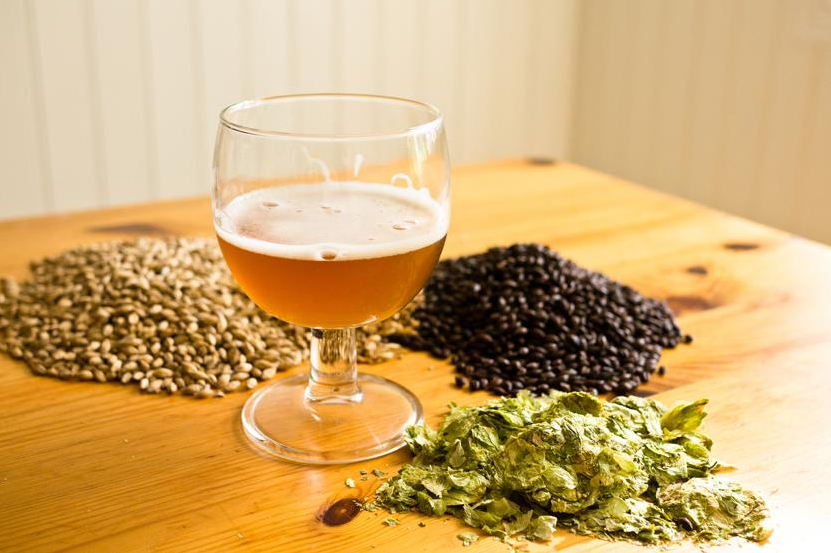
\includegraphics[width=90mm]{cover_image}
	\end{center}
}
\author{\Huge Kenneth E. Bellock \\ \\ \LARGE ken@bellock.net \\[1.5cm] Aprill 11, 2016 - TBD \\[1.5cm] This Journal is intended for personal use only.}
\maketitle

\printindex
\printglossaries
\glsaddall
\tableofcontents

\mainmatter

%------------------------------------------------------------------------------
%------------------------------------------------------------------------------
\newday{20180520}\label{20180520}

\newentry[Arrival and Setup]{0800 Arrival and Setup}
\FloatBarrier{}

Arrived at Damon Gunther's house for an introduction to beer brewing.  Damon already had his equipment setup (Figure~\ref{fig:setup}), in the driveway, and tools and ingredients laid out on a folding table (Figure~\ref{fig:tools}), inside the garage.  The end goal of this process is a homebrew clone of the Widmer Brothers Brewing Company Snowplow Milk Stout.

\begin{figure}[H]
\begin{minipage}{0.48\textwidth}
  \centering
  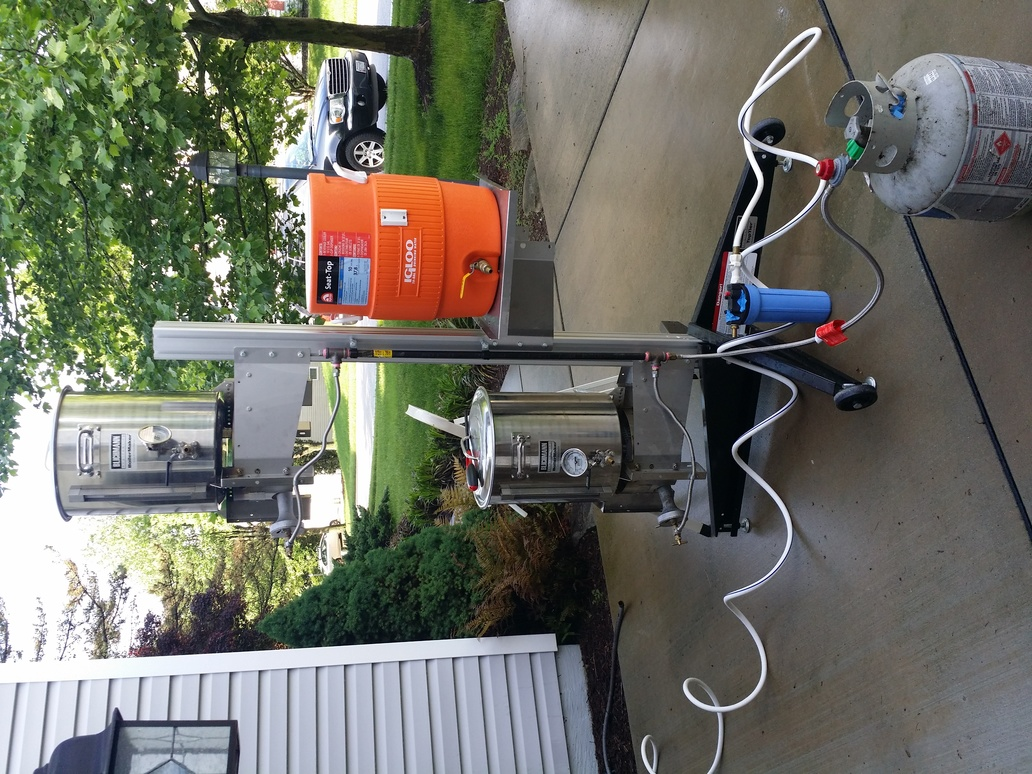
\includegraphics[angle=270,origin=c,width=\textwidth]{IMG_20180520_083244_reduced}
  \caption{Gravity feed brewing setup}\label{fig:setup}
\end{minipage}\hfill
\begin{minipage}{0.48\textwidth}
  \centering
  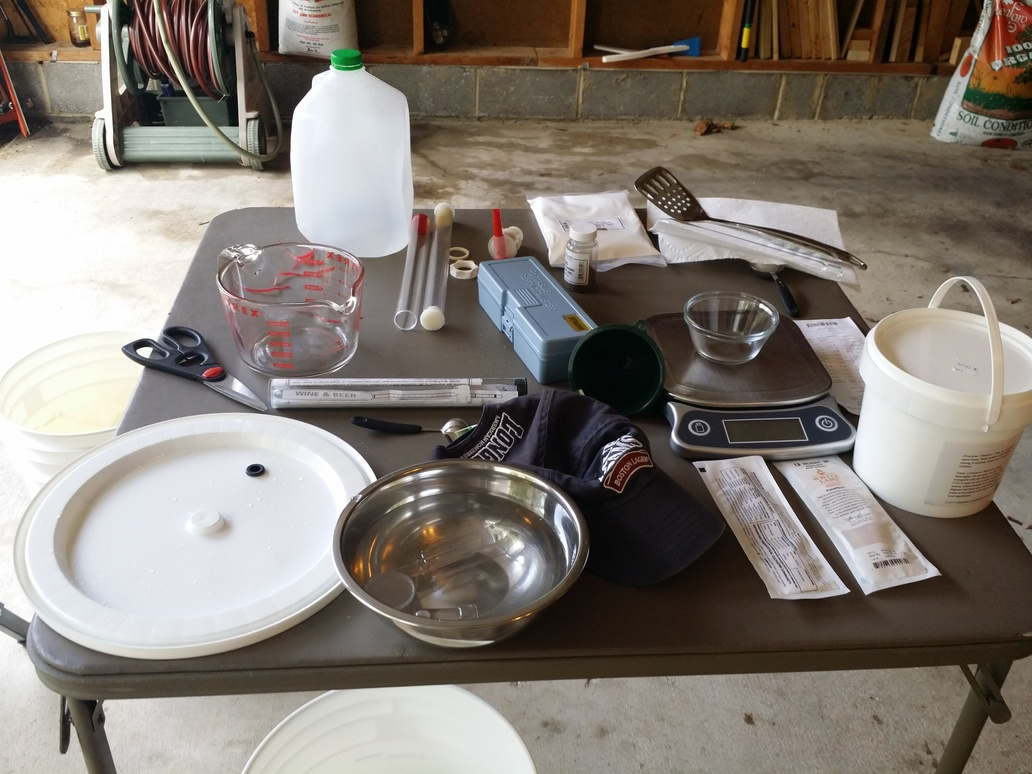
\includegraphics[width=\textwidth]{IMG_20180520_092957_reduced}
  \caption{Tools}\label{fig:tools}
\end{minipage}
\end{figure}

\FloatBarrier{}
\clearpage
%------------------------------------------------------------------------------
\newentry[Boil Filtered Water]{0830 Boil Filtered Water}\FloatBarrier{}

The top pot in Figure~\ref{fig:setup} is used to boil the \gls{strike water}, and also provides the heated \gls{sparge water} later in the process.  The \gls{strike water} must be heated to \SI{158} - \SI{173}\degree{}F.  When the strike water infuses with the grains to form the mash, the temperature will drop.  The ideal temperature range for the mash is \SI{148} - \SI{158}\degree{}F.  The temperature guage in Figure~\ref{fig:temp} is used to ensure the correct temperature of the water.

\begin{figure}[H]
  \centering
  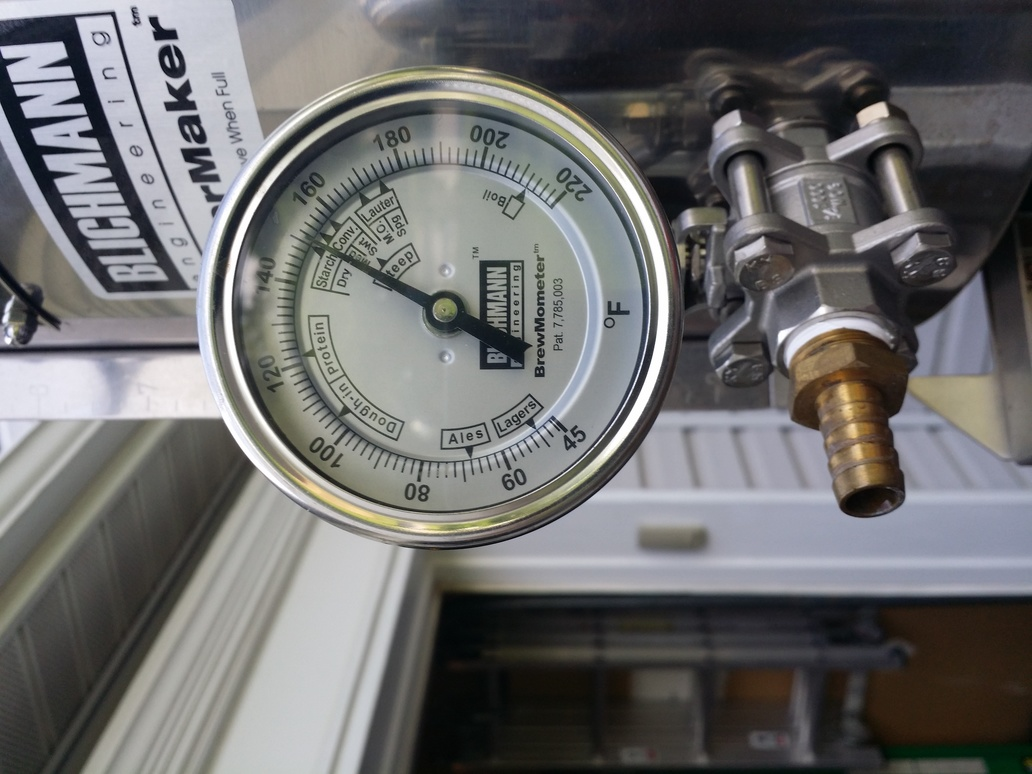
\includegraphics[angle=270,origin=c,width=0.5\textwidth]{IMG_20180520_083252_reduced}
  \caption{Temperature Guage}\label{fig:temp}
\end{figure}

\FloatBarrier{}
\clearpage
%------------------------------------------------------------------------------
\newentry[Mash In]{0845 Mash In}\FloatBarrier{}

Heated water goes in mash tun, also called the lautering tun.  All grains in the ingredients list \cref{subfig:flakedoats,subfig:tworow,subfig:crystalsixty,subfig:carapils,subfig:wheat,subfig:roastedbarley,subfig:black}, are stirred into the hot water in the lautering tun with the large stirring spoon. Check temperature in igloo. Desired temperatures will vary by recipie.  Start the timer for one hour, and start heating more water.

\begin{figure}[H]
\centering
\begin{subfigure}[b]{.245\textwidth}
  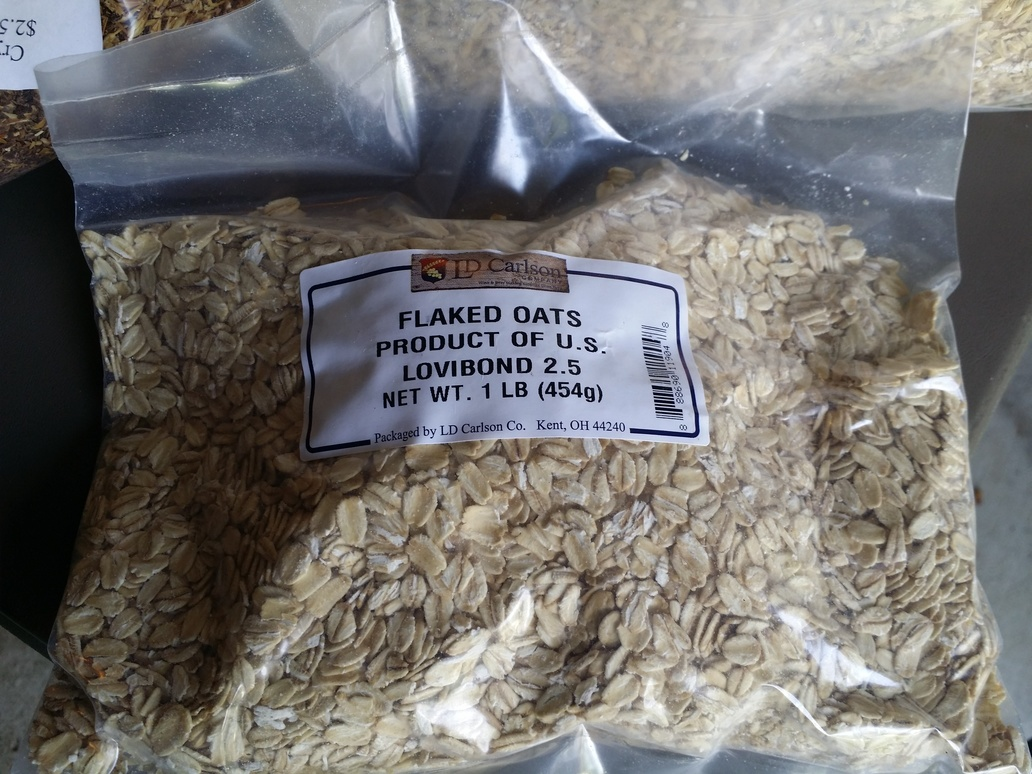
\includegraphics[width=\textwidth]{IMG_20180520_083053_reduced}
  \caption{Flaked Oats}\label{subfig:flakedoats}
\end{subfigure}
\begin{subfigure}[b]{.245\textwidth}
  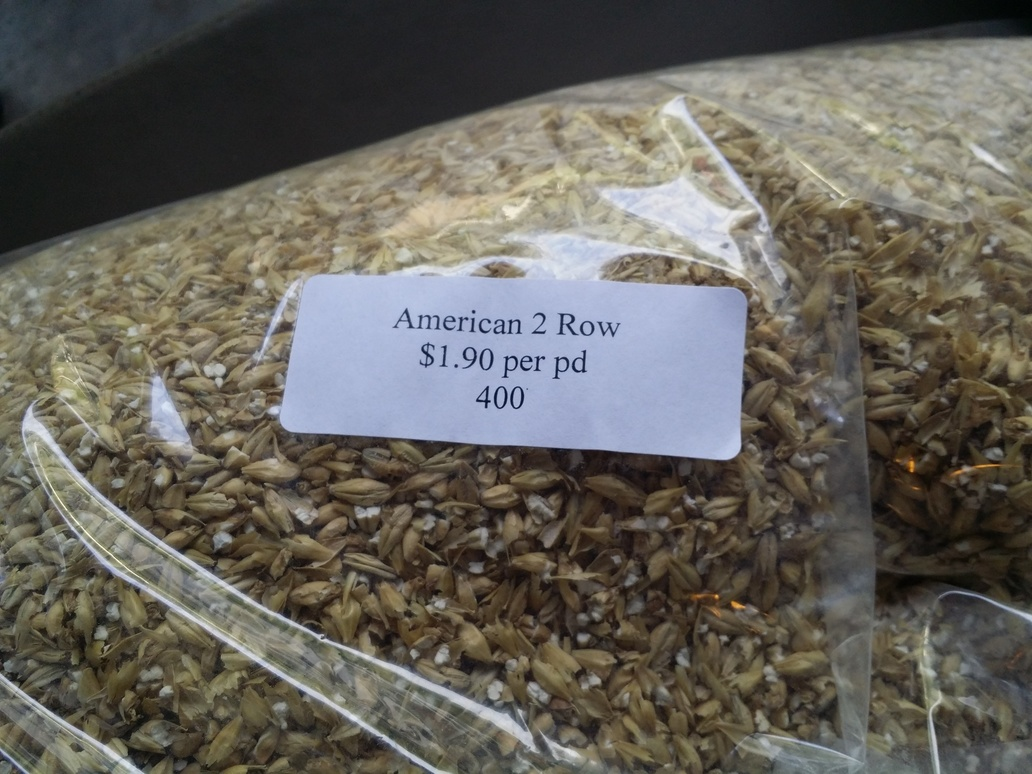
\includegraphics[width=\textwidth]{IMG_20180520_083103_reduced}
  \caption{American 2 Row}\label{subfig:tworow}
\end{subfigure}
\begin{subfigure}[b]{.245\textwidth}
  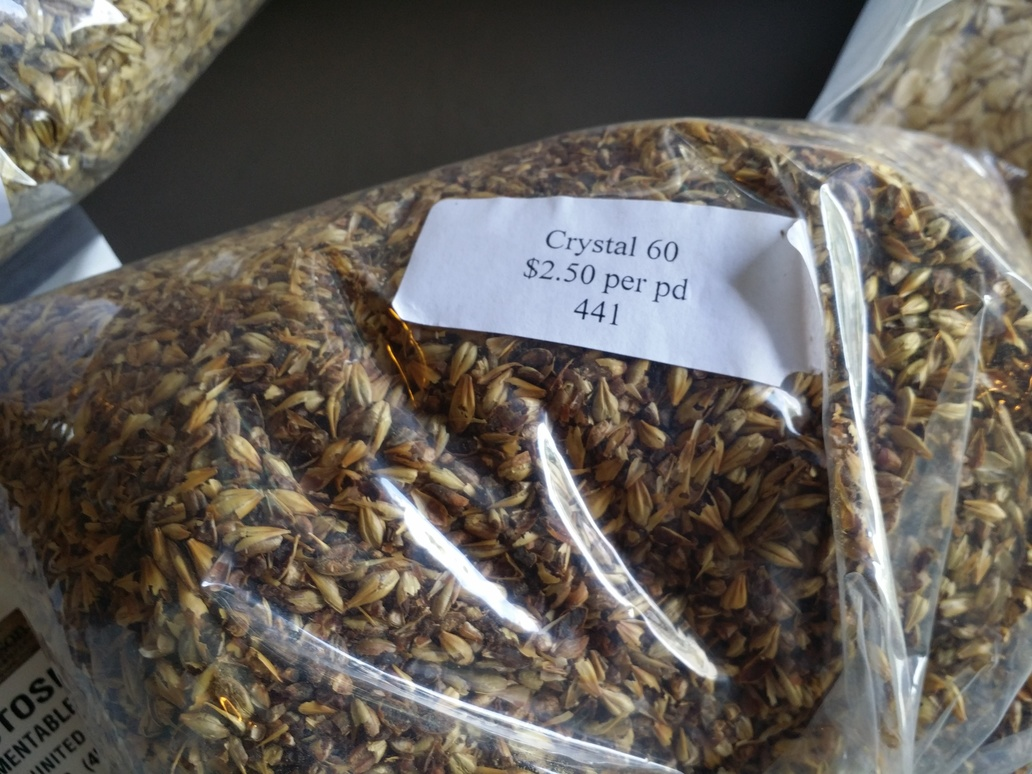
\includegraphics[width=\textwidth]{IMG_20180520_083110_reduced}
  \caption{Crystal 60}\label{subfig:crystalsixty}
\end{subfigure}
\begin{subfigure}[b]{.245\textwidth}
  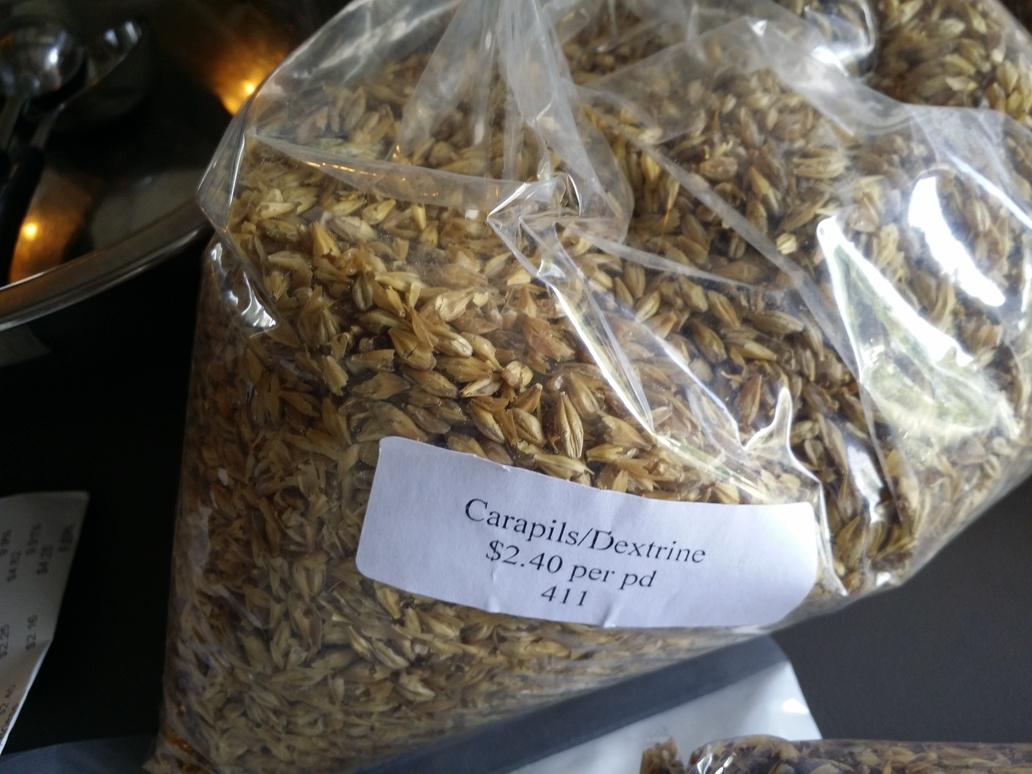
\includegraphics[width=\textwidth]{IMG_20180520_083114_reduced}
  \caption{Carapils/Dextrine}\label{subfig:carapils}
\end{subfigure}

\begin{subfigure}[b]{.245\textwidth}
  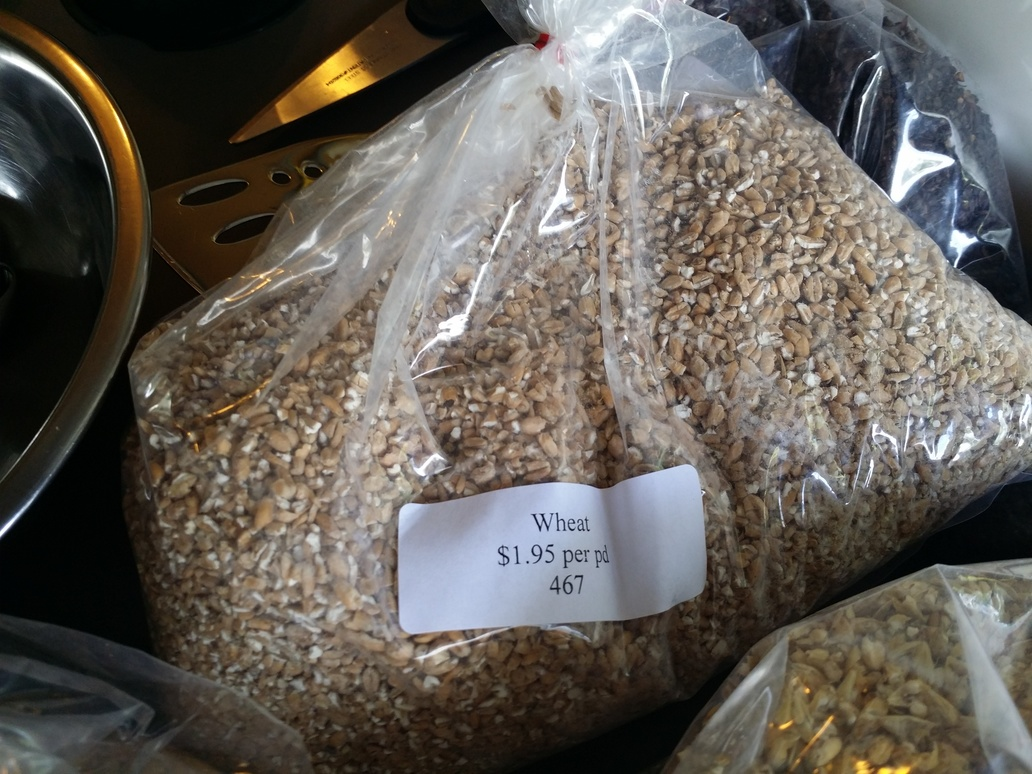
\includegraphics[width=\textwidth]{IMG_20180520_083120_reduced}
  \caption{Wheat}\label{subfig:wheat}
\end{subfigure}
\begin{subfigure}[b]{.245\textwidth}
  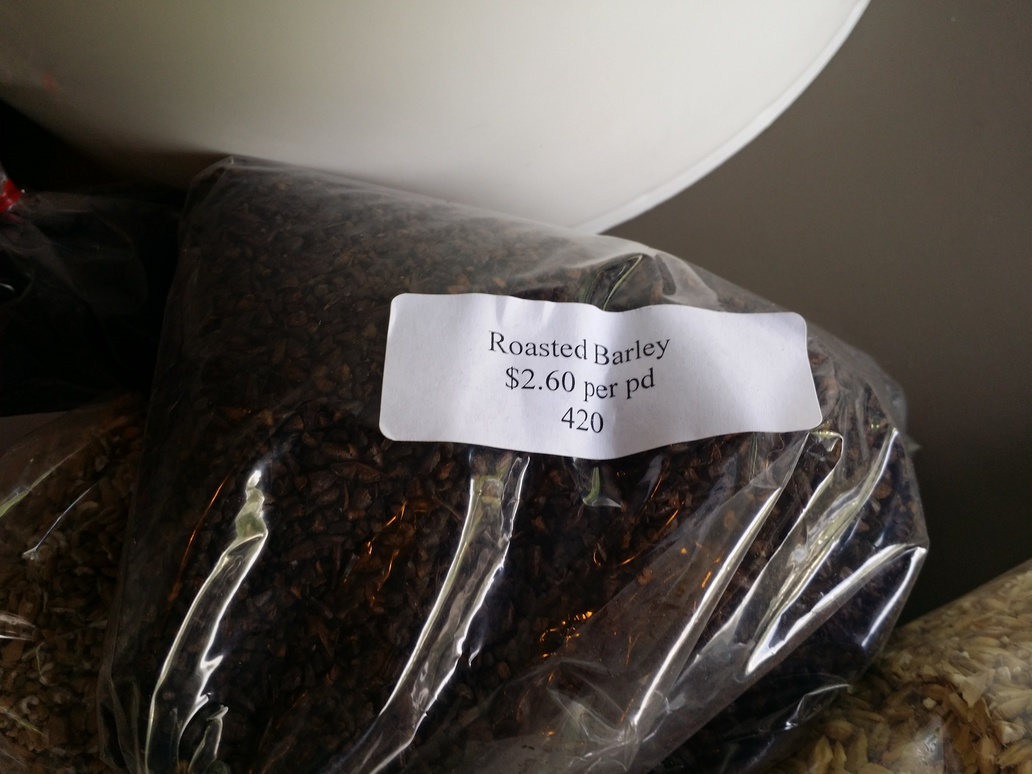
\includegraphics[width=\textwidth]{IMG_20180520_083130_reduced}
  \caption{Roasted Barley}\label{subfig:roastedbarley}
\end{subfigure}
\begin{subfigure}[b]{.245\textwidth}
  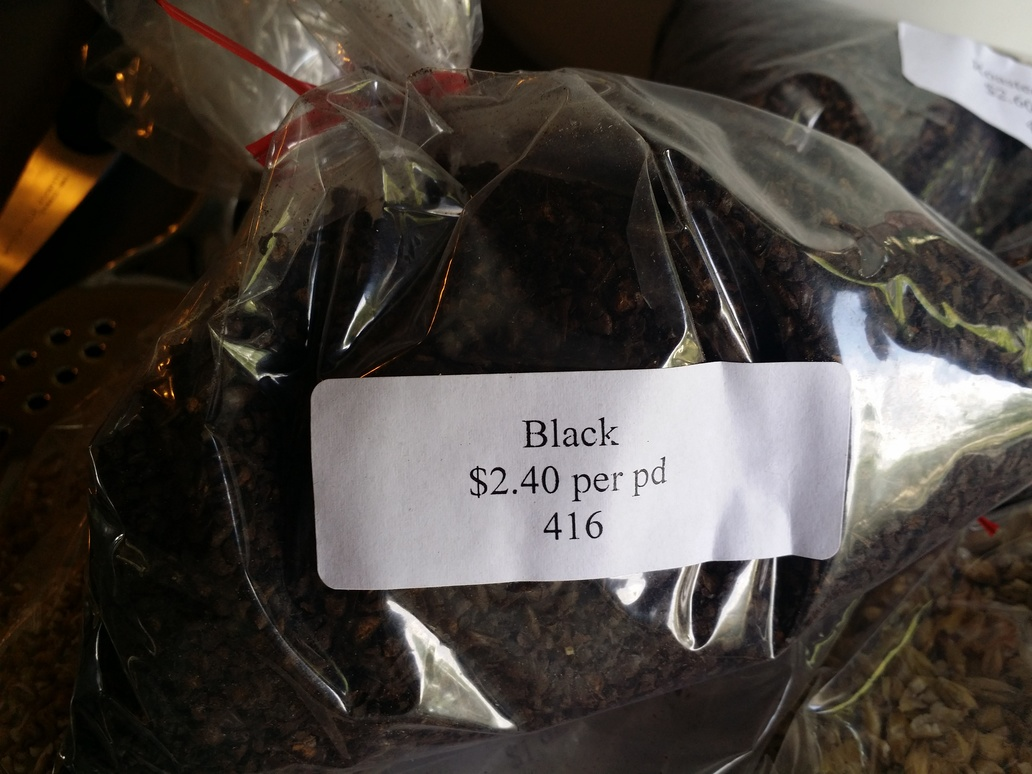
\includegraphics[width=\textwidth]{IMG_20180520_083135_reduced}
  \caption{Black}\label{subfig:black}
\end{subfigure}

\begin{subfigure}[b]{.245\textwidth}
  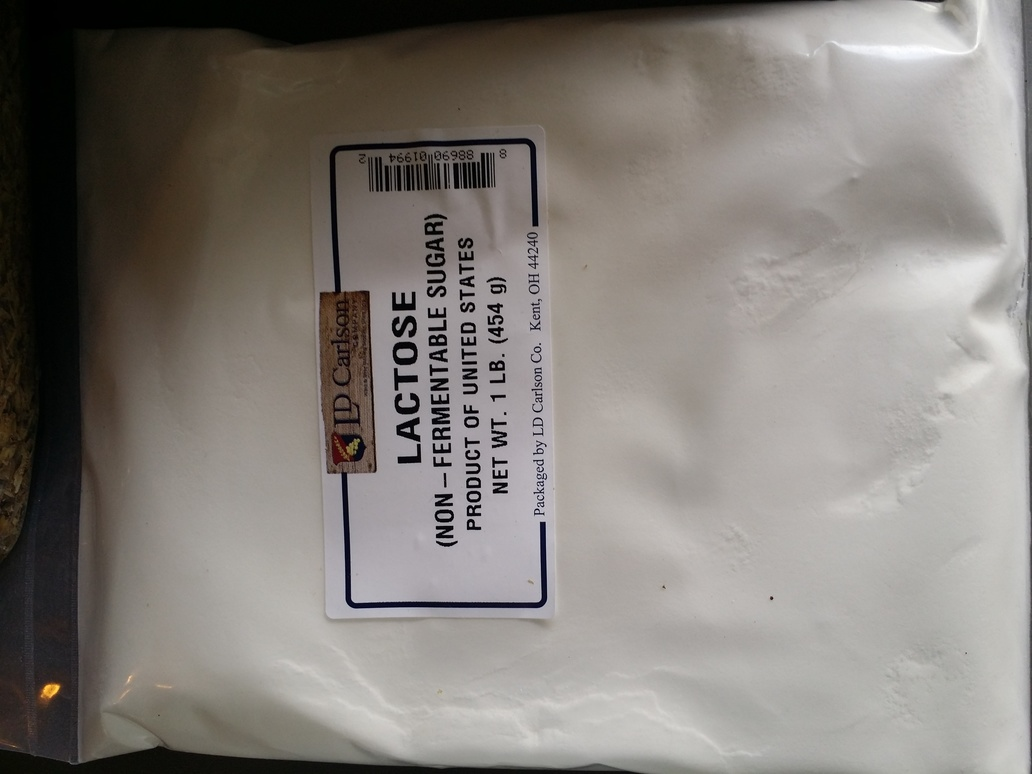
\includegraphics[angle=270,origin=c,width=\textwidth]{IMG_20180520_083204_reduced}
  \caption{Lactose}\label{subfig:lactose}
\end{subfigure}
\begin{subfigure}[b]{.245\textwidth}
  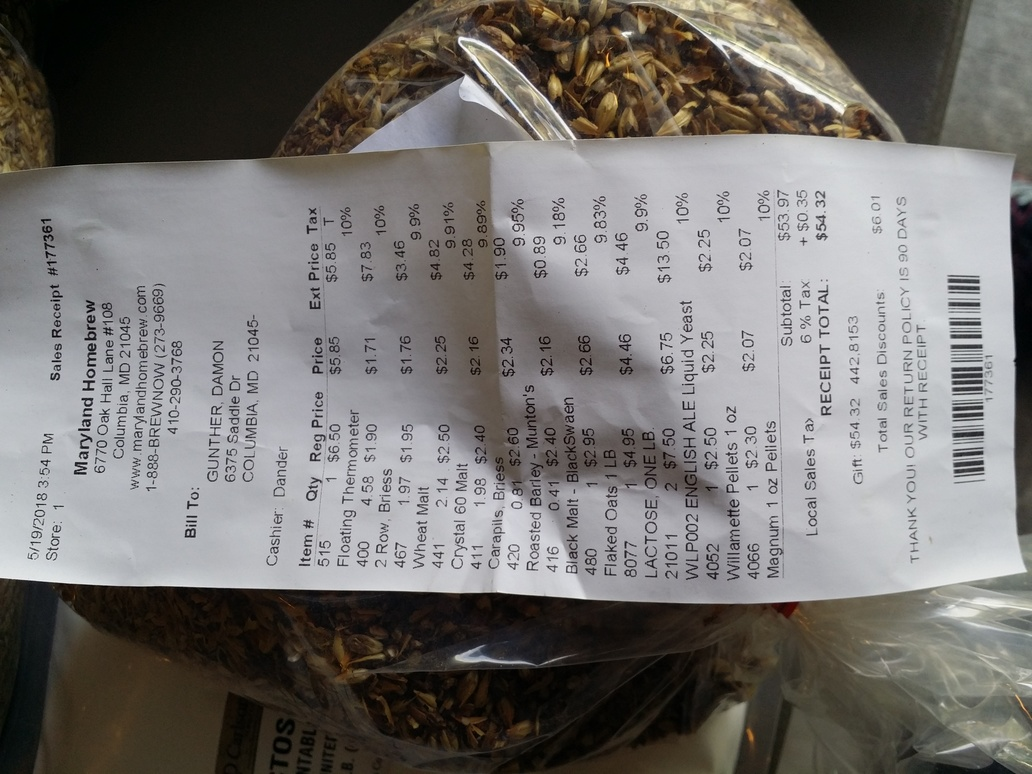
\includegraphics[angle=270,origin=c,width=\textwidth]{IMG_20180520_083145_reduced}
  \caption{Reciept}\label{subfig:receipt}
\end{subfigure}
\caption{Ingredients}\label{subfig:ingredients}
\end{figure}

\begin{figure}[H]
  \centering
  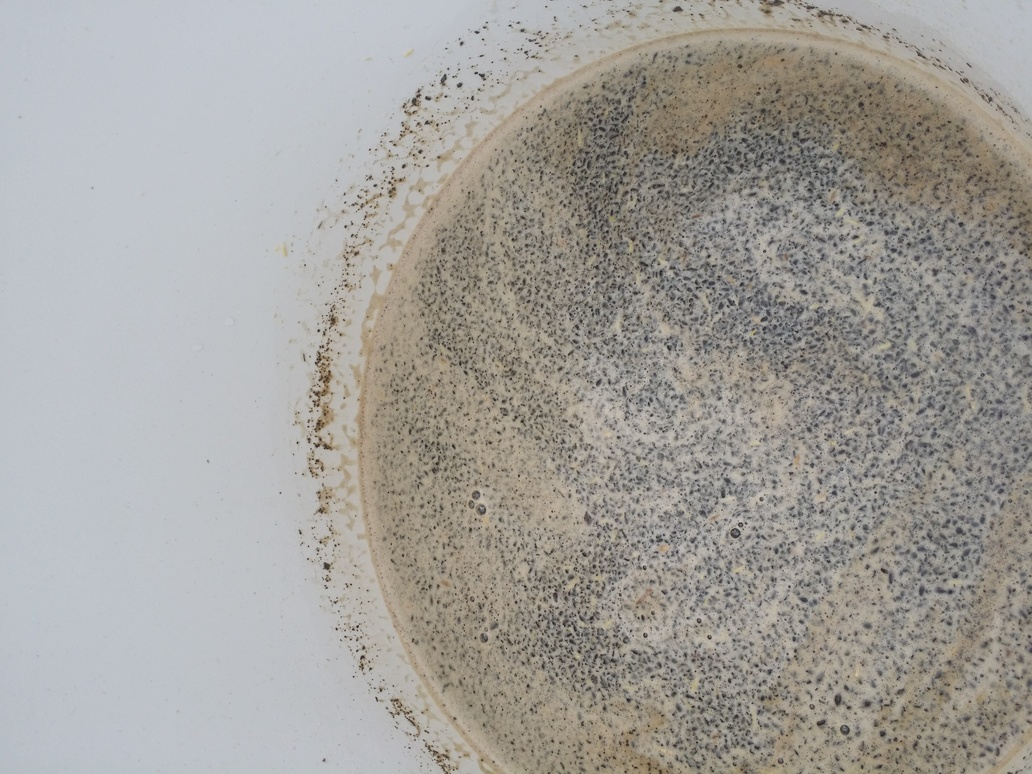
\includegraphics[width=0.5\textwidth]{IMG_20180520_084614_reduced}
  \caption{Mash}\label{fig:mash}
\end{figure}

\FloatBarrier{}
%------------------------------------------------------------------------------
\newentry[Cleaning]{0850 Cleaning}\FloatBarrier{}

Sanitize the primary firmentation bucket, tools and air-lock.  With the sanitizing compound in Figure~\ref{fig:sanitizer}, no rinse in plain water is required to remove the sanitizer.

\begin{figure}[H]
\begin{minipage}{0.45\textwidth}
  \centering
  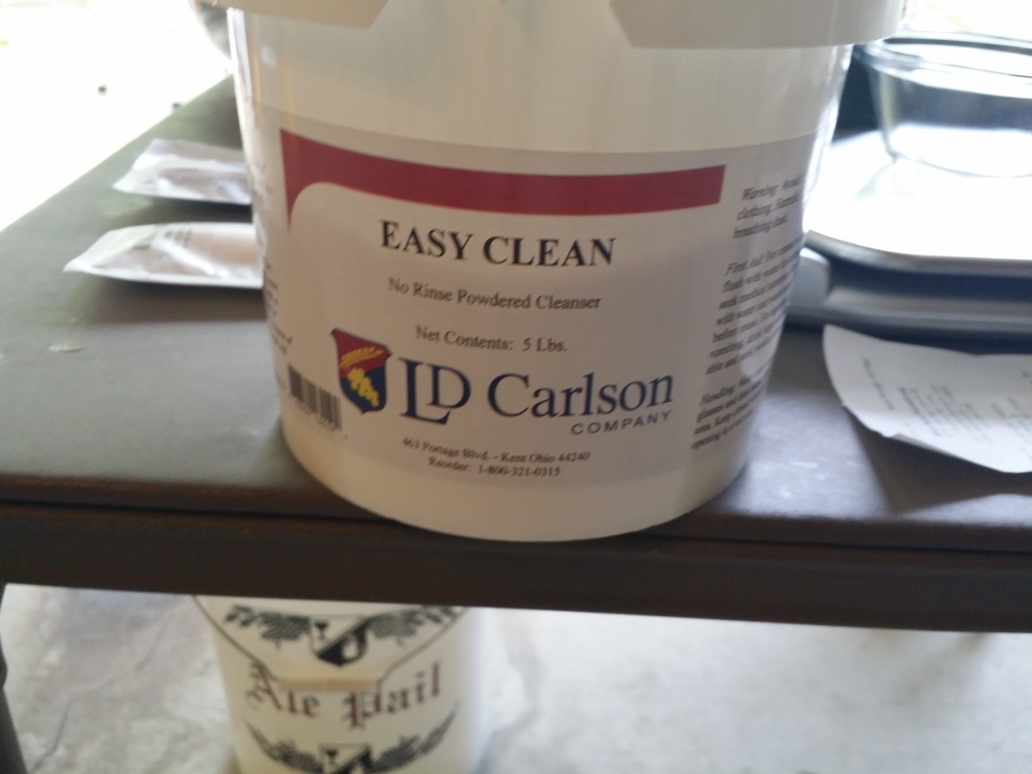
\includegraphics[width=\textwidth]{IMG_20180520_093004_reduced}
  \caption{No rinse sanitizer}\label{fig:sanitizer}
\end{minipage}\hfill
\begin{minipage}{0.45\textwidth}
  \centering
  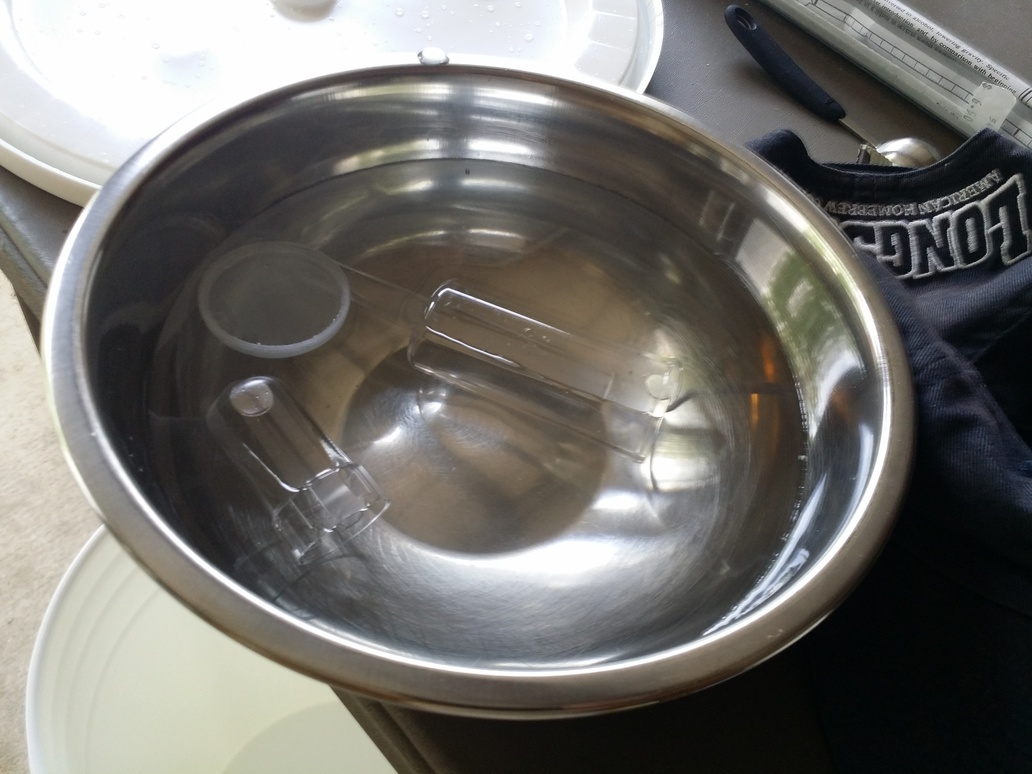
\includegraphics[width=\textwidth]{IMG_20180520_093016_reduced}
  \caption{Air-Lock Sanitizing}\label{fig:airlock}
\end{minipage}
\end{figure}

\FloatBarrier{}
%------------------------------------------------------------------------------
\newentry[Sparging]{0955 Sparging}\FloatBarrier{}

When timer was done wort was drawn from igloo silcock into a temporary container and then poured back into the igloo through top until the wort coming out of the silcock no longer had little bits of grain, as shown in Figure~\ref{fig:rinse}.  This cycles the fluid and places the little bits on top of the grain pile so they will be filtered out during sparging.

Setup the hot water sprayer on top of the igloo, being fed from the top pot as shown in Figure~\ref{fig:sparging}, and slowly spray water while draining out bottom into lower pan, Figure~\ref{fig:transfer}.  Go slow, this should take an hour.  As it starts to fill start heating the lower container, it will need to get to a rolling boil.  Figure~\ref{fig:gravitydrain} shows the sparging by draining heated water from the top container into the lautering tun, and then the wort being drained from the lautering tun into the lower boil pot.

\begin{figure}[H]
\centering
\begin{subfigure}[b]{.245\textwidth}
  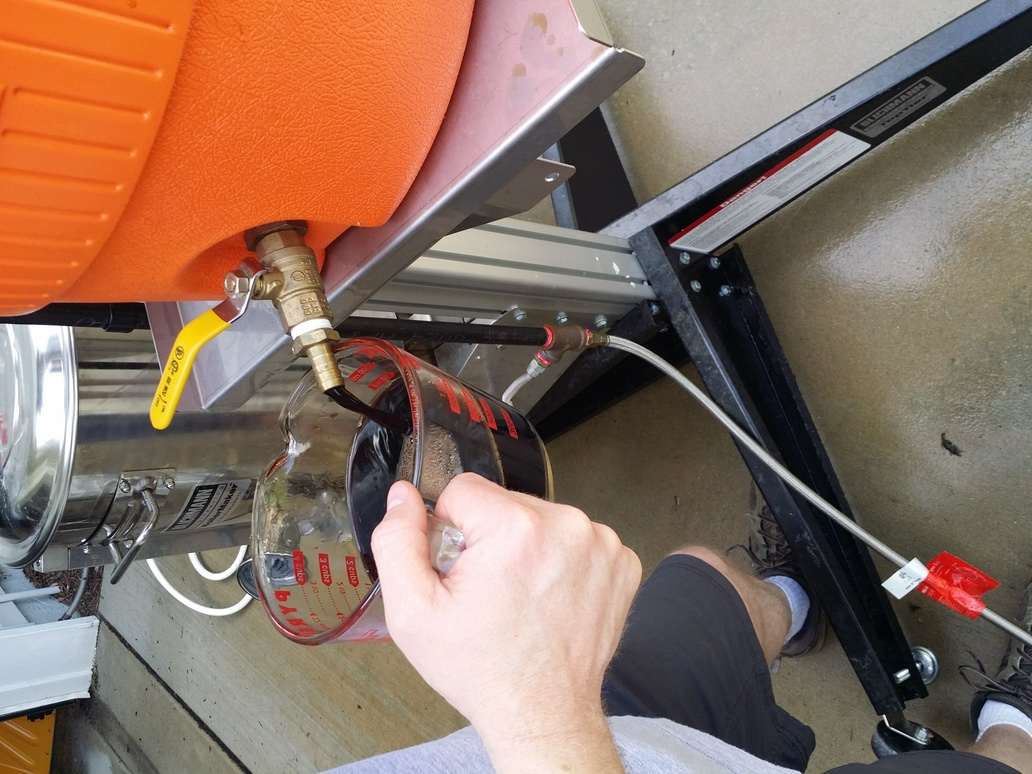
\includegraphics[angle=270,origin=c,width=\textwidth]{IMG_20180520_095406_reduced}
  \caption{Rinse}\label{fig:rinse}
\end{subfigure}
\begin{subfigure}[b]{.245\textwidth}
  \centering
  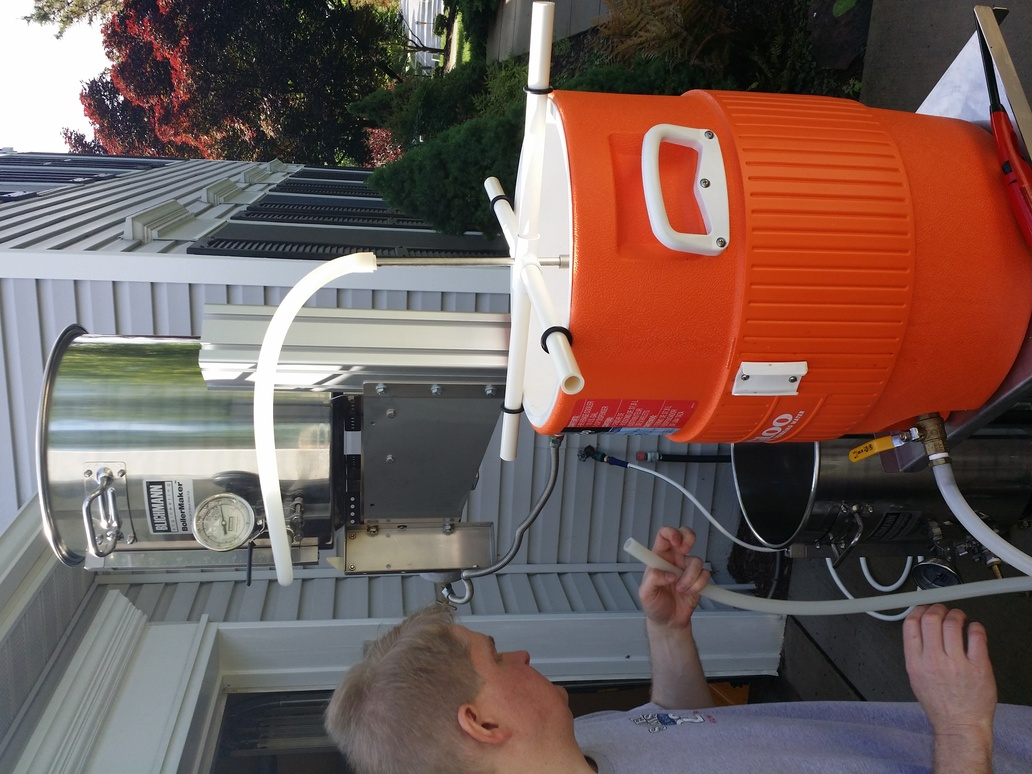
\includegraphics[angle=270,origin=c,width=\textwidth]{IMG_20180520_100013_reduced}
  \caption{Sparging}\label{fig:sparging}
\end{subfigure}
\begin{subfigure}[b]{.245\textwidth}
  \centering
  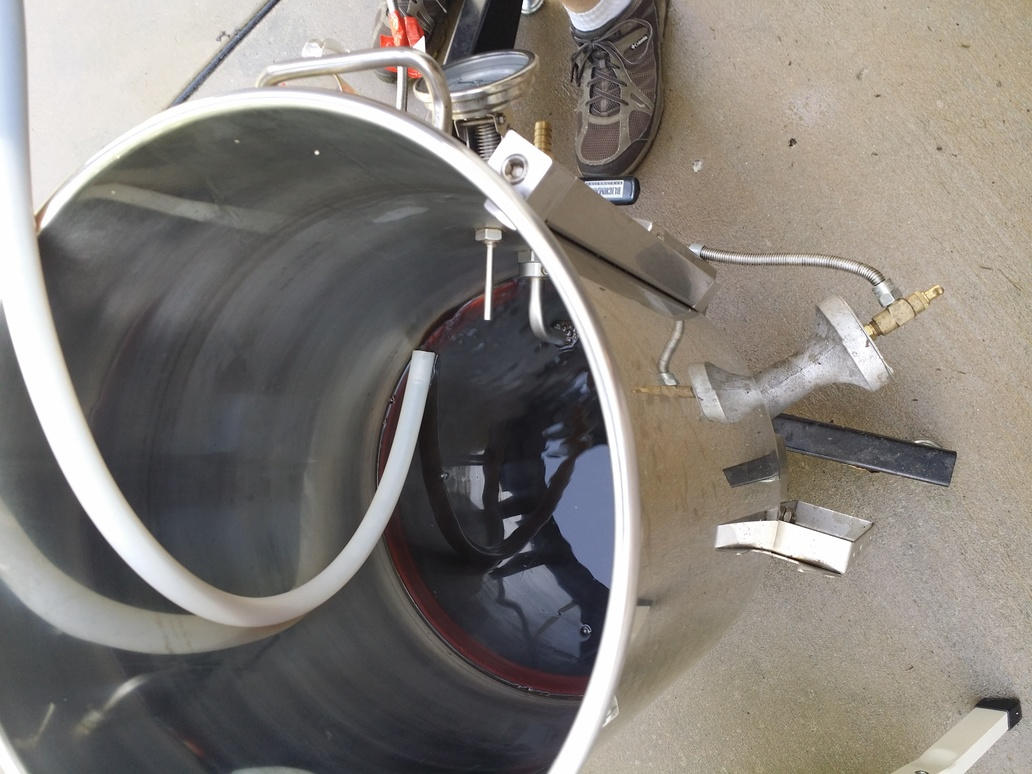
\includegraphics[angle=270,origin=c,width=\textwidth]{IMG_20180520_100206_reduced}
  \caption{Transfer for boil}\label{fig:transfer}
\end{subfigure}
\begin{subfigure}[b]{.245\textwidth}
  \centering
  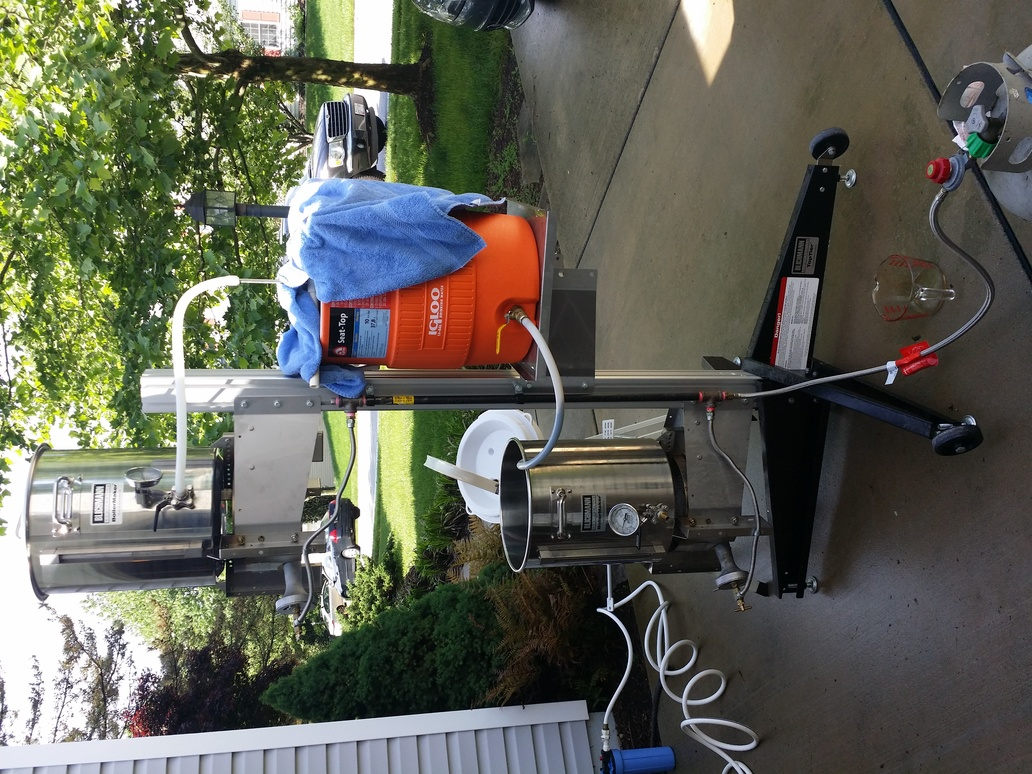
\includegraphics[angle=270,origin=c,width=\textwidth]{IMG_20180520_100432_reduced}
  \caption{Draining by gravity}\label{fig:gravitydrain}
\end{subfigure}
\caption{Sparging Process}\label{subfig:spargingprocess}
\end{figure}

\FloatBarrier{}
%------------------------------------------------------------------------------
\newentry[Boil Wort]{0955 Boil Wort}\FloatBarrier{}

Bring the wort to a rolling boil as shown in Figure~\ref{fig:boil}.  Measure out hops using a scale, and add to the boil according to recepie.

\begin{figure}[H]
  \centering
  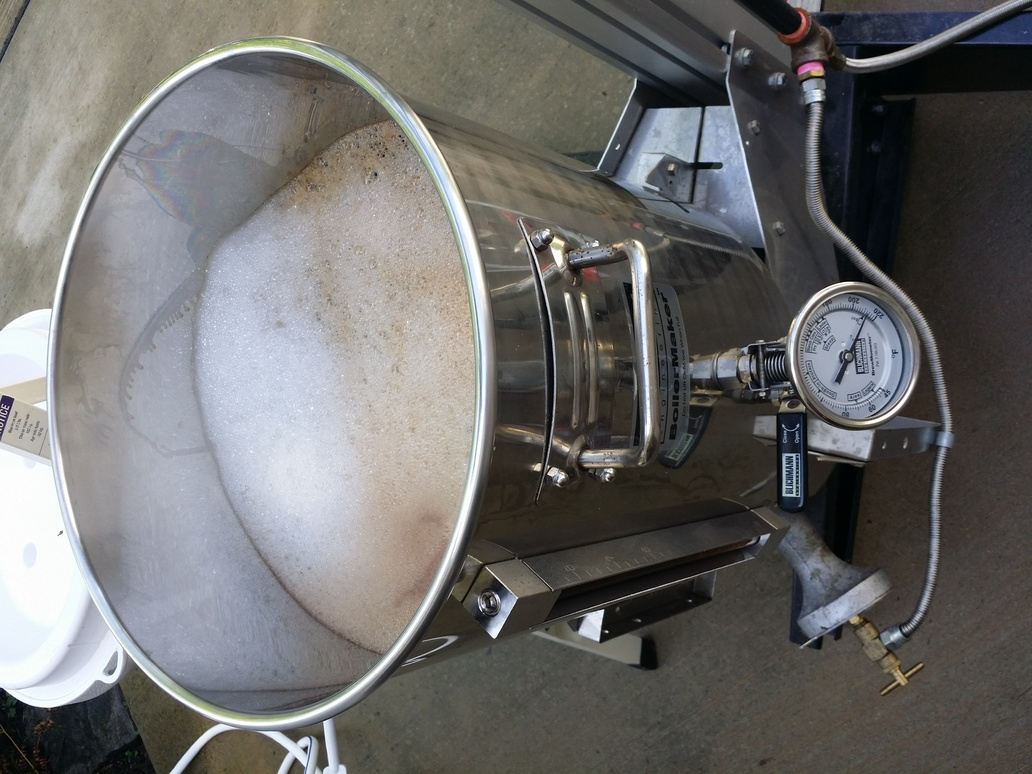
\includegraphics[angle=270,origin=c,width=0.95\textwidth]{IMG_20180520_110050_reduced}
  \caption{Boil}\label{fig:boil}
\end{figure}

\FloatBarrier{}
\clearpage
%------------------------------------------------------------------------------
\newentry[Cooling]{0955 Cooling}\FloatBarrier{}

Add the cooling coil at the end of boil but for several minutes while the boil to roll to sanitize the coil as shown in Figure~\ref{fig:cooling}.  The heat was turned off and coolling was begun by turning on the water to the cooling coil. The goal is to bring the temperature down to 70 degrees as quick as possible.

\begin{figure}[H]
  \centering
  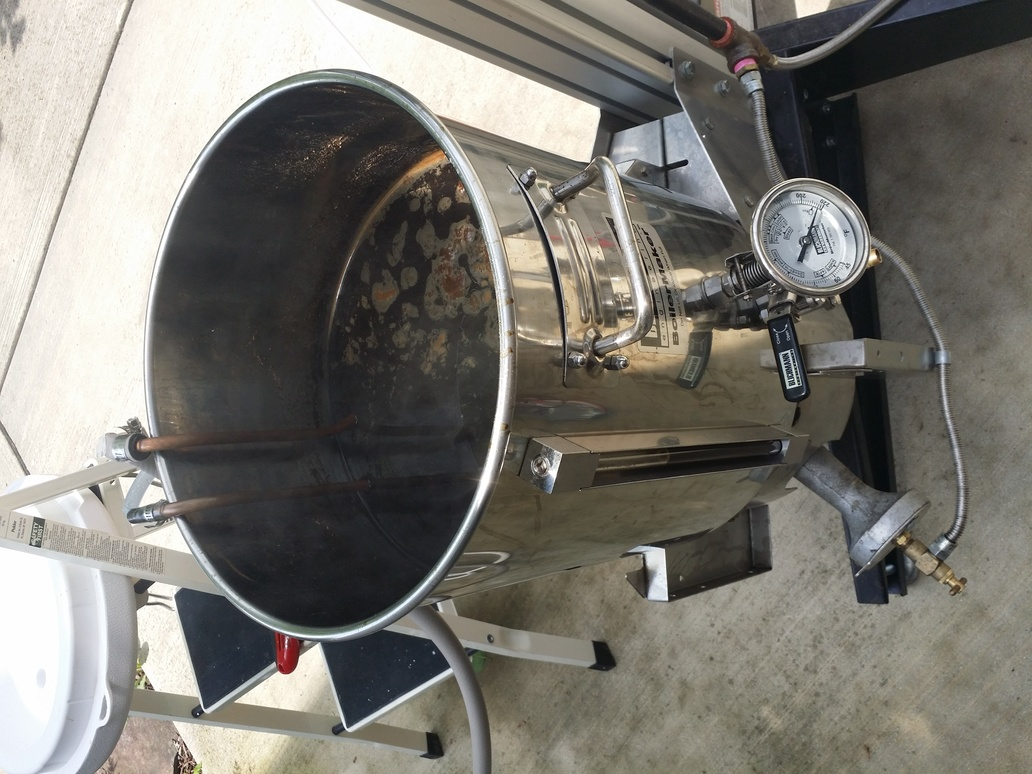
\includegraphics[angle=270,origin=c,width=0.95\textwidth]{IMG_20180520_123637_reduced}
  \caption{Cooling}\label{fig:cooling}
\end{figure}

\FloatBarrier{}
\clearpage
%------------------------------------------------------------------------------
\newentry[Transfer to Primary Firmentation Bucket]{0955 Transfer to Primary Firmentation Bucket}\FloatBarrier{}

Transfer to 5 gallon bucket as shown in Figure~\ref{fig:primary}, measure weight.

\begin{figure}[H]
  \centering
  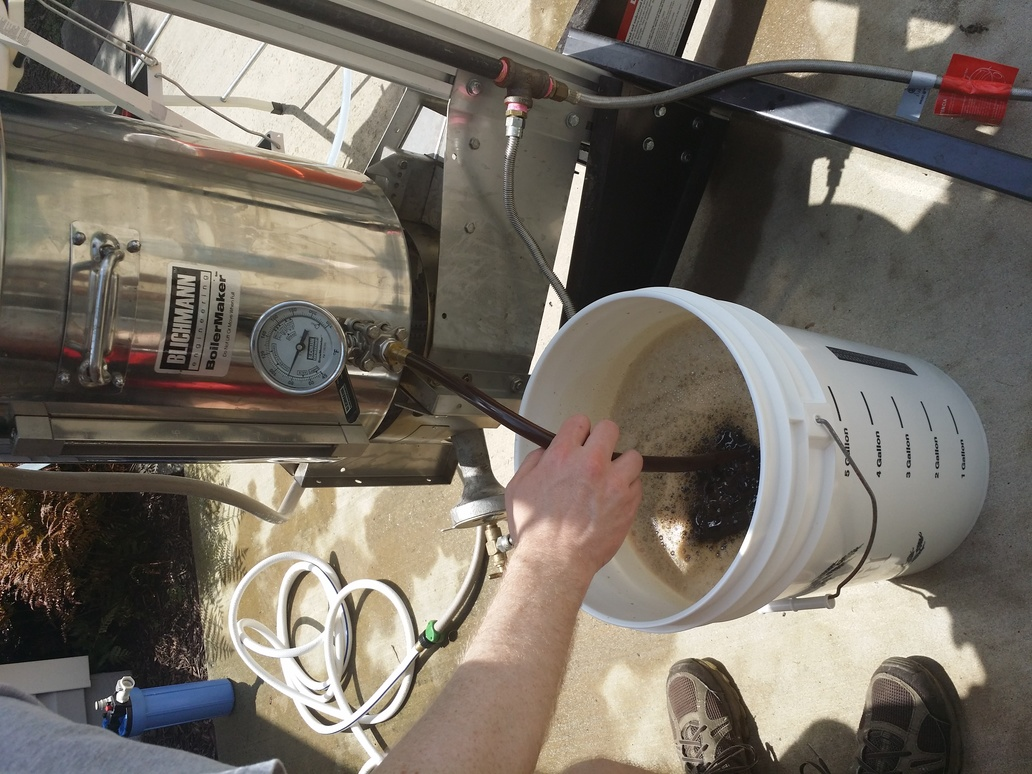
\includegraphics[angle=270,origin=c,width=\textwidth]{IMG_20180520_132938_reduced}
  \caption{Primary firmentation bucket}\label{fig:primary}
\end{figure}

\FloatBarrier{}
%------------------------------------------------------------------------------
\newentry[Aeration]{0955 Aeration}\FloatBarrier{}

Stir to aerate with oxygen for 10 to 15 minutes as shown in Figure~\ref{fig:aeration}. Watch the texture of the bubbles, as you are nearing finished, the bubbles will live longer.

\begin{figure}[H]
  \centering
  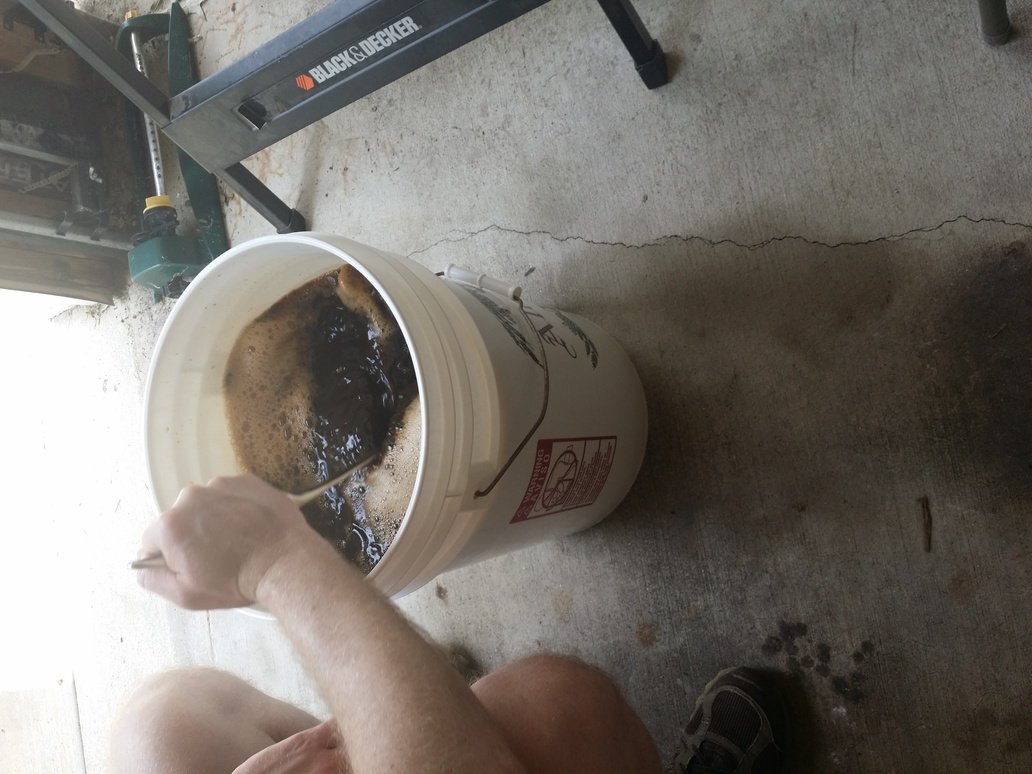
\includegraphics[angle=270,origin=c,width=\textwidth]{IMG_20180520_133334_reduced}
  \caption{Aeration}\label{fig:aeration}
\end{figure}

\FloatBarrier{}
%------------------------------------------------------------------------------
\newentry[Add Yeast]{0955 Add Yeast}\FloatBarrier{}

Sanitize the top edge of the bucket, sanitize yeast packet and scissors, open yeast and add to the bucket.  Stir in the yeast. Seal the bucket. Add one way valve for pressure escape and pour some sanitizer in the one way valve.

\begin{figure}[H]
  \centering
  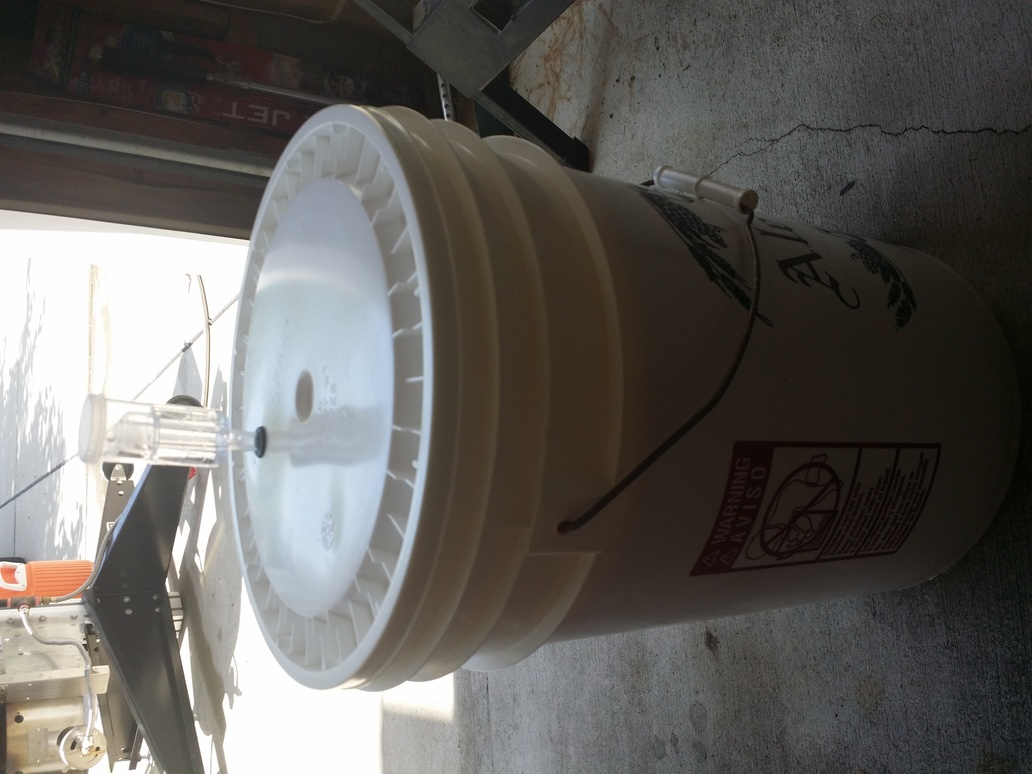
\includegraphics[angle=270,origin=c,width=0.95\textwidth]{IMG_20180520_134840_reduced}
  \caption{Sealed for primary firmentation}\label{fig:sealed}
\end{figure}

%------------------------------------------------------------------------------
%------------------------------------------------------------------------------
\newday{20180901}

\newentry[Homebrew System Planning]{0800 Homebrew System Planning}\FloatBarrier{}

After tasting the results of the~\hyperref[20180520]{May 20\textsuperscript{th}} brew, I have decided to start homebrewing myself.  The past several weeks I have been reading up on the processes and techniques and trying to sort out which of the many configurations for homebrewing will both work well for me, and provide an opportunity for fusion with other hobbies of mine, such as microcontroller programming, to be expanded later by automation.

\begin{table}[h!]
\centering
\begin{tabularx}{\textwidth}{clrcX}
    \toprule
    \multicolumn{1}{c}{\textbf{ID}} &\multicolumn{1}{c}{\textbf{Name}} & \multicolumn{1}{c}{\textbf{Price}} & \textbf{Quantity} & \multicolumn{1}{c}{\textbf{Link}} \\
    1 & Brewer's Edge Mash and Boil & \$299.99 & 1 & {\tiny\url{https://amazon.com/gp/product/B075NNZ3KT}} \\
    2 & Fermentation Lid & \$34.16 & 1 & {\tiny\url{https://amazon.com/gp/product/B077Y3RNK7}} \\
    3 & Sparge Water Heater & \$156.66 & 1 & {\tiny\url{https://amazon.com/gp/product/B01D05UHXQ}} \\
    4 & Chugger Pump & \$154.99 & 1 & {\tiny\url{https://amazon.com/gp/product/B01NCKU3ZC}} \\
    5 & Plate Chiller & \$89.99 & 1 & {\tiny\url{https://amazon.com/gp/product/B06Y44CS86}} \\
    6 & 5 Gallon Soda Keg & \$132.88 & 1 & {\tiny\url{https://amazon.com/gp/product/B00YREN4GM}} \\
    7 & Spoon & \$8.85 & 1 & {\tiny\url{https://amazon.com/gp/product/B001D6KF8M}} \\
    8 & Fermentation Bucket & \$36.73 & 1 & {\tiny\url{https://amazon.com/gp/product/B072B9X98X}} \\
    9 & Airlock & \$3.00 & 1 & {\tiny\url{https://amazon.com/gp/product/B000E60G2W}} \\
    10 & Ball Valve & \$22.90 & 1 & {\tiny\url{https://amazon.com/gp/product/B071GKPB6B}} \\
    11 & Wort Aerator & \$6.48 & 1 & {\tiny\url{https://amazon.com/gp/product/B00ODSS5J8}} \\
    12 & 3-Way Ball Valve & \$25.89 & 1 & {\tiny\url{https://amazon.com/gp/product/B07G72DFVQ}} \\
    13 & Male Hose Barb & \$8.50 & 1 & {\tiny\url{https://amazon.com/gp/product/B075VF861W}} \\
    14 & Female Hose Barb & \$7.25 & 1 & {\tiny\url{https://amazon.com/gp/product/B0064OJDUO}} \\
    15 & \#10 Rubber Stopper & \$4.95 & 1 & {\tiny\url{https://amazon.com/gp/product/B0057JB9XG}} \\
    17 & Silicone Tubing & \$19.55 & 1 & {\tiny\url{https://amazon.com/gp/product/B000FMWU38}} \\
    \bottomrule
\end{tabularx}
\caption{Parts List}\label{tab:partslist}
\end{table}

\tikzset{
block/.style = {draw, fill=white, rectangle, minimum height=3em, minimum width=3em},
tmp/.style  = {coordinate}, 
sum/.style= {draw, fill=white, circle, node distance=1cm},
input/.style = {coordinate},
output/.style= {coordinate},
pinstyle/.style = {pin edge={to-,thin,black}},
number/.style = {anchor=west,shape=circle,draw,inner sep=2pt}
}
\begin{figure}[H]
\centering
\begin{tikzpicture}[auto, node distance=2cm,>=latex']
    % Nodes
    \node (mashandboil) {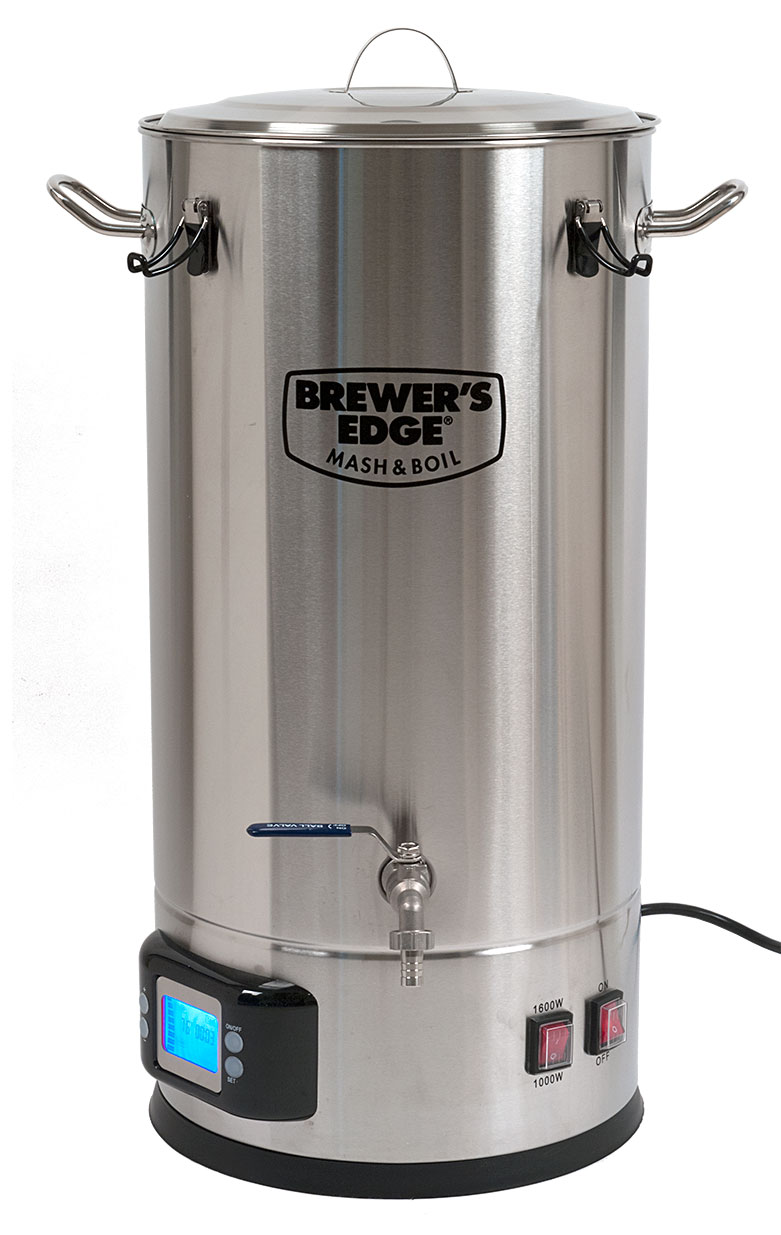
\includegraphics[width=1in]{mashandboil}};
    \node [left of=mashandboil, node distance=1in] (spargewater) {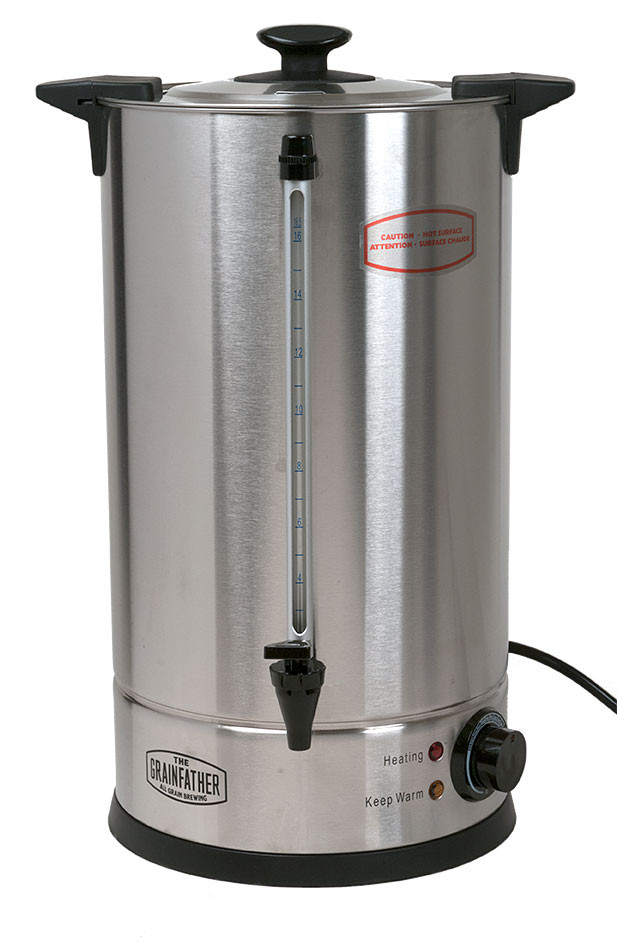
\includegraphics[width=1in]{spargewater}};
    \node [sum,below of=spargewater,node distance=1in] (swout) {};
    \node [sum,above of=mashandboil,node distance=1in] (mbin) {};
    \node [sum,below of=mashandboil,node distance=1in] (mbout) {};
    \node [right of=mbout] (chugger) {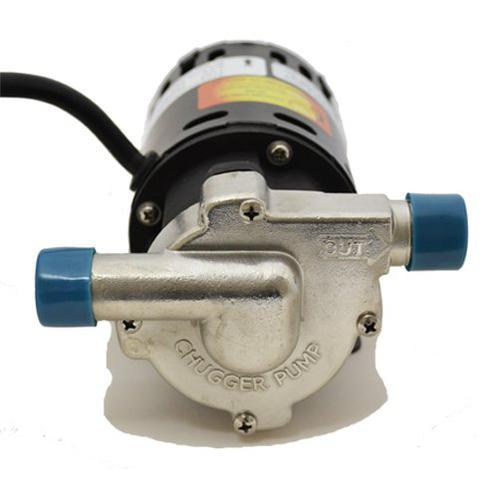
\includegraphics[width=0.5in]{chugger}};
    \node [spdt,above of=chugger,rotate=90] (switch1) {};
    \node [right of=switch1,yshift=0.6cm] (platechiller) {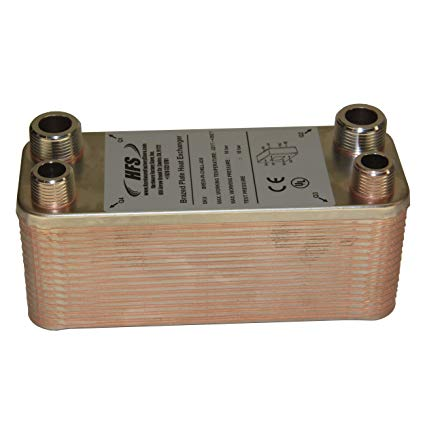
\includegraphics[width=0.5in]{platechiller}};
    \node [above of=platechiller] (tapwater) {Tap Water};
    \node [below of=platechiller] (drain) {Drain};
    \node [output,right of=platechiller] (pcout) {};
    
    % Lines
    \draw (mashandboil) -- (mbin);
    \draw (mashandboil) -- (mbout);
    \draw (spargewater) -- (swout);
    \draw (swout) -- (mbout);
    \draw (mbout) -- (chugger);
    \draw (chugger) -- (switch1.in);
    \draw (switch1.out 1) |- (mbin);
    \draw (switch1.out 2) -| (platechiller.west);
    \draw (platechiller) -- (pcout);
    \draw (platechiller) -- (tapwater);
    \draw (platechiller) -- (drain);
    \draw (pcout) |- (mbin);

    % Annotations
    \node [number] (1)  at (-1.45, 0.3) {1};
    \node [number] (3)  at (-4.0,  0.3) {3};
    \node [number] (4)  at ( 2.3, -3.1) {4};
    \node [number] (5)  at ( 3.1,  0.9) {5};
    \node [number] (10) at (-3.3, -3.0) {10};
    \node [number] (11) at (-1.0,  2.6) {11};
    \node [number] (12) at ( 1.9,  0.5) {12};
\end{tikzpicture}
\caption{Proposed Homebrew Configuration}\label{fig:config}
\end{figure}
\clearpage

The following is a proposed schedule for brew day using the configuration in Figure~\ref{fig:config}.

\begin{enumerate}
    \item Pour a beer.
    \item Add filtered water to sparge water heater and mash tun.
    \item Set mash tun to heat water to strike water temperature.
    \item Set sparge water heater to boil.
    \item Wait for strike water to come to temperature.
    \item Set flow control valve to bypass plate chiller.
    \item Mash in grain ingredients.
    \item Set timer.
    \item Start pump, and circulate at a slow rate into the top of the grain bed.
    \item Clean primary firmentation bucket, airlock, spoon, scissors, yeast package.
    \item Wait until timer is ended.
    \item Lift the grain tube to upper position.
    \item Close the valve on the mash tun, and open the sparge water valve, slowly sparging with  calculated needed water.
    \item Close the valve on the sparge water heater, remove the grain tube and place in primary firmentation bucket until ready to clean.
    \item Set mash tun to boil temperature.
    \item Add hops as instructed in the recipie.
    \item Clean grain tube.
    \item Set flow control valve to inline plate chiller.
    \item At five minutes left in the boil, leave the tap water valve closed, and open the valve on the mash tun to circulate boiling wort through the plate chiller to sanitize.
    \item Turn off mash tun heating element.
    \item Turn on tap water.
    \item Continue chilling till desired temperature is reached.
    \item Set flow control valve to bypass plate chiller, turn off tap water.
    \item Add yeast.
    \item Let pump circulate to aerate the wort and stir in yeast.
    \item Stop pump.
    \item Move wort aerator to primary firmentation bucket.
    \item Start pump and transfer wort from mash tun to primary firmentation bucket.
    \item Add airlock to primary firmentation bucket.
    \item Remove wort aerator from hose and place hose in drain.
    \item Set flow control valve to inline plate chiller.
    \item Open sparge water heater valve and drain remaining hot water through the plate chiller and into the drain.
    \item Turn off pump.
    \item Disconnect line from sparge water heater and re-connect to compressed air line.
    \item Open compressed air line just enough to purge water from lines, pump, and plate chiller.
    \item Pour another beer.
    \item Clean mash tun.
\end{enumerate}

The plan is to force carbonate in cornelius kegs.
%------------------------------------------------------------------------------
\newday{20180920}

\begin{figure}[H]
  \centering
  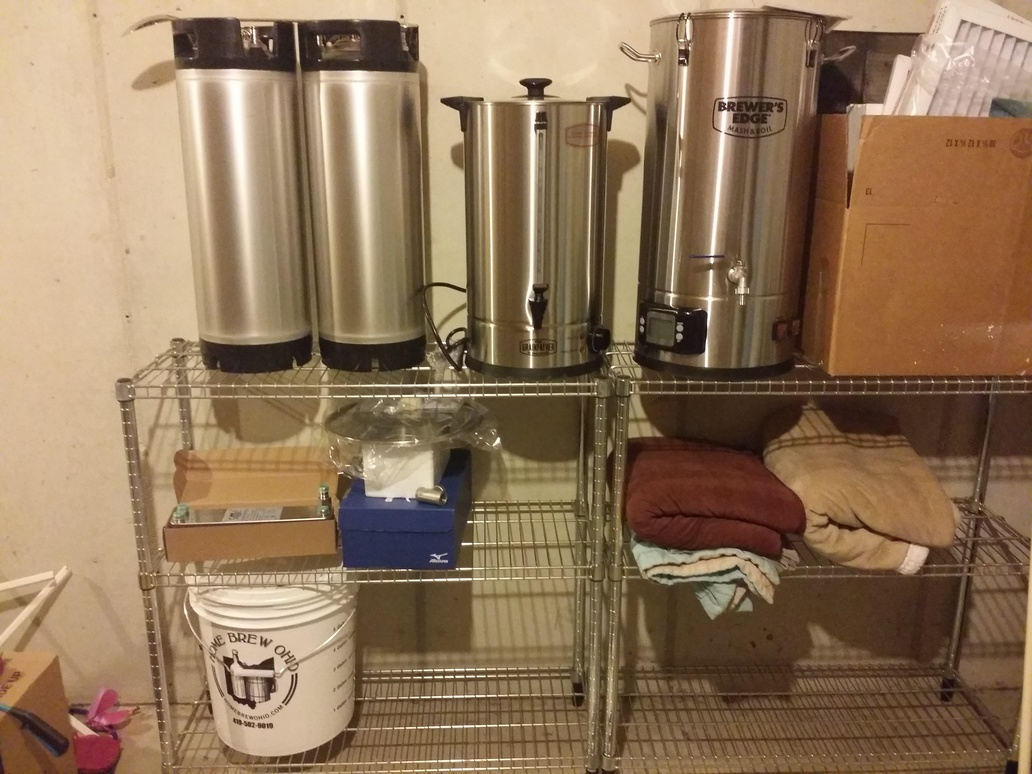
\includegraphics[angle=0,origin=c,width=\textwidth]{IMG_20180920_212437_reduced}
  \caption{Beginning Assembly of Brewing Equipment}\label{fig:temp}
\end{figure}

%------------------------------------------------------------------------------
\newday{20181014}

\newentry[Test Run]{0800 Test Run}\FloatBarrier{}


\begin{figure}[H]
  \centering
  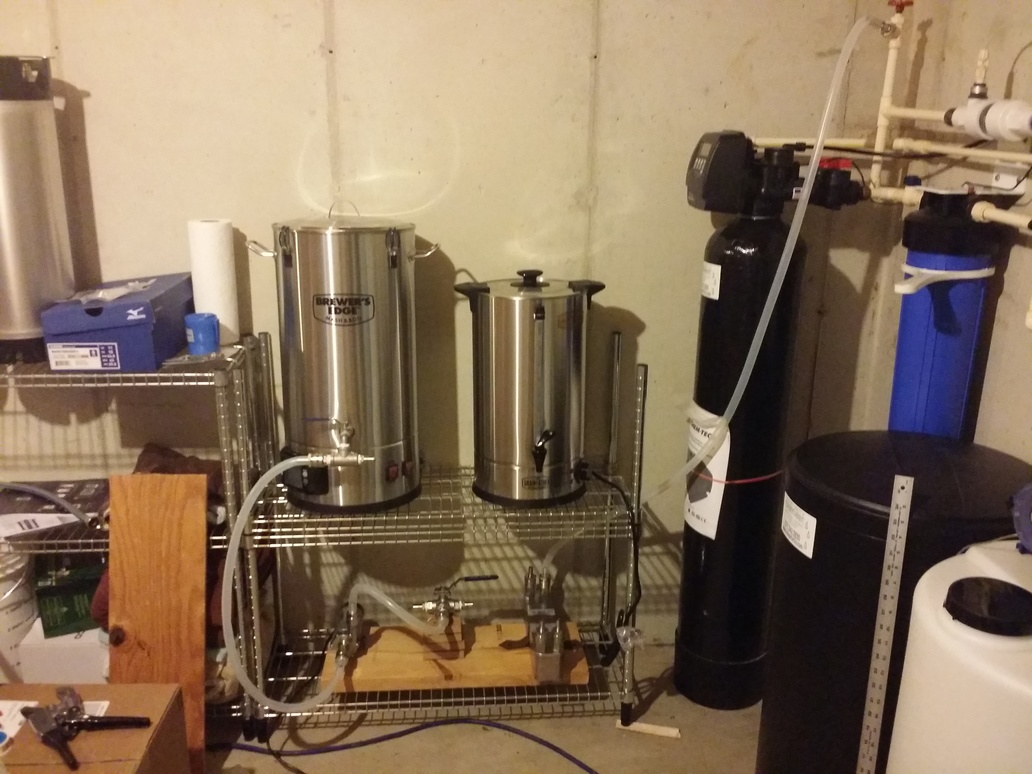
\includegraphics[angle=0,origin=c,width=\textwidth]{IMG_20181014_113442_reduced}
  \caption{Beginning Assembly of Brewing Equipment}\label{fig:temp}
\end{figure}

Running the system with just water today to evaluate the design and brew plan 
\begin{itemize}
    \item 
\end{itemize}

%------------------------------------------------------------------------------
\newday{20181028}

\newentry[Sparge Water Heater Modification]{0800 Sparge Water Heater Modification}\FloatBarrier{}

The sparge water heater has a plastic nozzle that will not attach to the quick hose disconnects easily.  I do not want to remove it, as it has an integrated water level indicator.  The temperature setting for heat is only in Celcius, and is not calibaratablle, so the plan is to install a good temperature probe next to the heat level dial, and a spicot with a fitting ready to receive a quick disconnect fitting on the other side of the existing spicot.

Using a step drill bit, shown below the thermometer in figure~\ref{fig:swm:drilled}, a \nicefrac{7}{8}\textsuperscript{th} inch hole was drilled for the ball valve (left of the existing spicot), and a \nicefrac{1}{2} inch hole was drilled for the temperature guage (right of the existing spicot).  I think a hole punch would have worked better as the step drill created a mess on the inside of shavings, and left the inside hole perimeter with large shards of razor sharp metal pressed in from the hole.  Instructions with some step drill bits recommend drilling from the other side to clean up the hole, but that was not possible with the locations of these holes inside the container.  Instead the holes were cleaned up by turning the step drill bit by hand on the inside, and by using files.  The resulting hole was not as clean as I would have liked it to be, or precise, even though figure~\ref{fig:swm:drilled} looks pretty good, it was not possible to take a picture from the inside with any clarity.  Once the fittings were installed as shown in figure~\ref{fig:swm:installed}, there were no leaks, so the process worked well enough.  As shown installed in figure~\ref{fig:swm:drilled}, a quick connect addapter was placed on the ball valve.

\begin{figure}[H]
  \centering
  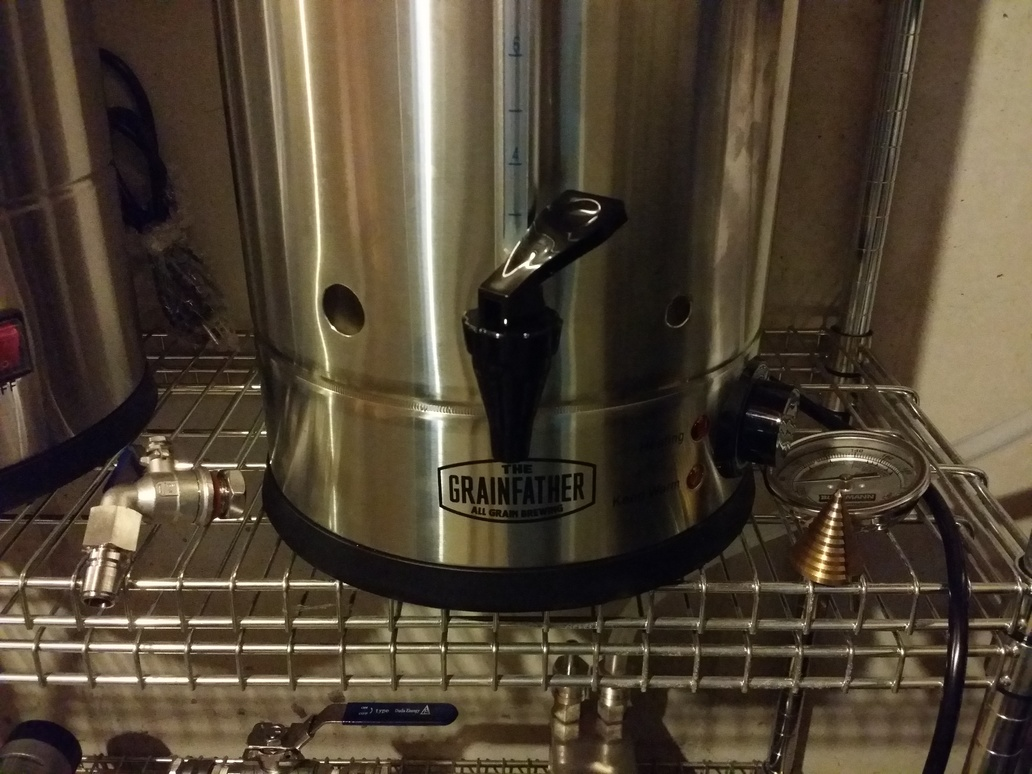
\includegraphics[angle=0,origin=c,width=\textwidth]{IMG_20181028_135028_reduced}
  \caption{Drilling Holes for Sparge Water Heater Modification}\label{fig:swm:drilled}
\end{figure}

\newentry[Test Run]{0800 Test Run}\FloatBarrier{}

\begin{figure}[H]
  \centering
  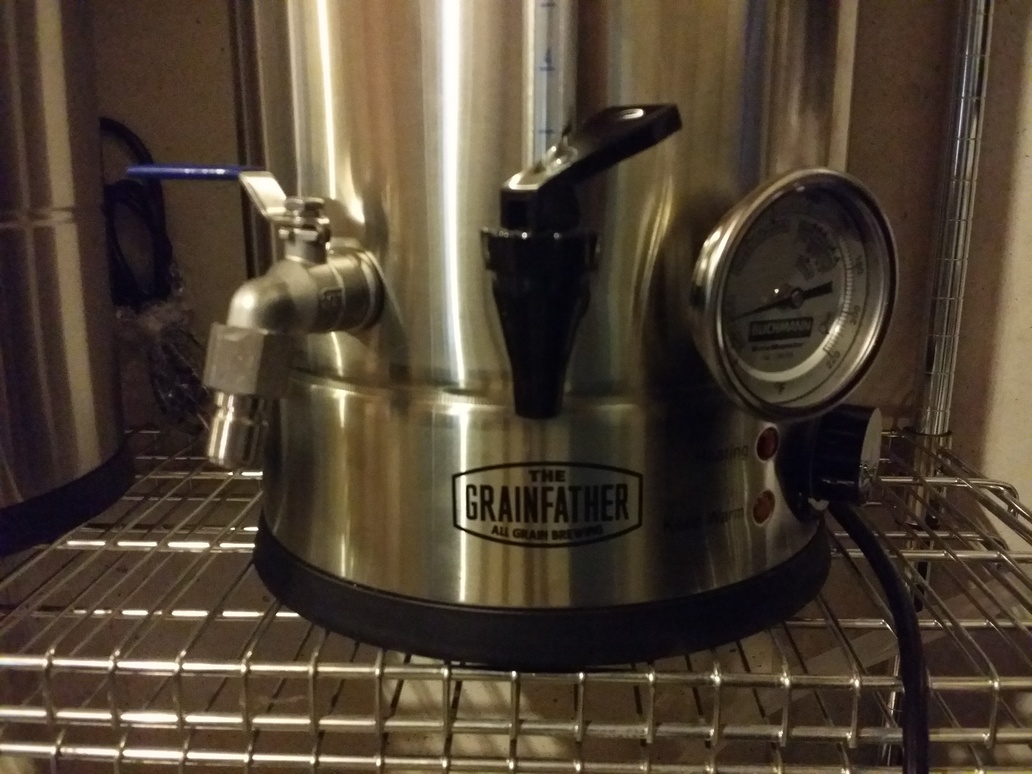
\includegraphics[angle=0,origin=c,width=\textwidth]{IMG_20181028_141228_reduced}
  \caption{Sparge Water Modifications Installed}\label{fig:swm:installed}
\end{figure}

%------------------------------------------------------------------------------
\newday{20181124}

\newentry[Homebrew Re-Design]{0800 Homebrew Re-Design}\FloatBarrier{}

After tasting the results of the~\hyperref[20180520]{May 20\textsuperscript{th}} brew, I have decided to start homebrewing myself.  The past several weeks I have been reading up on the processes and techniques and trying to sort out which of the many configurations for homebrewing will both work well for me, and provide an opportunity for fusion with other hobbies of mine, such as microcontroller programming, to be expanded later by automation.

\begin{table}[h!]
\centering
\begin{tabularx}{\textwidth}{clrcX}
    \toprule
    \multicolumn{1}{c}{\textbf{ID}} &\multicolumn{1}{c}{\textbf{Name}} & \multicolumn{1}{c}{\textbf{Price}} & \textbf{Quantity} & \multicolumn{1}{c}{\textbf{Link}} \\
    1 & Brewer's Edge Mash and Boil & \$299.99 & 1 & {\tiny\url{https://amazon.com/gp/product/B075NNZ3KT}} \\
    2 & Fermentation Lid & \$34.16 & 1 & {\tiny\url{https://amazon.com/gp/product/B077Y3RNK7}} \\
    3 & Sparge Water Heater & \$156.66 & 1 & {\tiny\url{https://amazon.com/gp/product/B01D05UHXQ}} \\
    4 & Chugger Pump & \$154.99 & 1 & {\tiny\url{https://amazon.com/gp/product/B01NCKU3ZC}} \\
    5 & Plate Chiller & \$89.99 & 1 & {\tiny\url{https://amazon.com/gp/product/B06Y44CS86}} \\
    6 & 5 Gallon Soda Keg & \$132.88 & 1 & {\tiny\url{https://amazon.com/gp/product/B00YREN4GM}} \\
    7 & Spoon & \$8.85 & 1 & {\tiny\url{https://amazon.com/gp/product/B001D6KF8M}} \\
    8 & Fermentation Bucket & \$36.73 & 1 & {\tiny\url{https://amazon.com/gp/product/B072B9X98X}} \\
    9 & Airlock & \$3.00 & 1 & {\tiny\url{https://amazon.com/gp/product/B000E60G2W}} \\
    10 & Ball Valve & \$22.90 & 1 & {\tiny\url{https://amazon.com/gp/product/B071GKPB6B}} \\
    11 & Wort Aerator & \$6.48 & 1 & {\tiny\url{https://amazon.com/gp/product/B00ODSS5J8}} \\
    12 & 3-Way Ball Valve & \$25.89 & 1 & {\tiny\url{https://amazon.com/gp/product/B07G72DFVQ}} \\
    13 & Male Hose Barb & \$8.50 & 1 & {\tiny\url{https://amazon.com/gp/product/B075VF861W}} \\
    14 & Female Hose Barb & \$7.25 & 1 & {\tiny\url{https://amazon.com/gp/product/B0064OJDUO}} \\
    15 & \#10 Rubber Stopper & \$4.95 & 1 & {\tiny\url{https://amazon.com/gp/product/B0057JB9XG}} \\
    17 & Silicone Tubing & \$19.55 & 1 & {\tiny\url{https://amazon.com/gp/product/B000FMWU38}} \\
    \bottomrule
\end{tabularx}
\caption{Parts List}\label{tab:partslist}
\end{table}

\tikzset{
block/.style = {draw, fill=white, rectangle, minimum height=3em, minimum width=3em},
tmp/.style  = {coordinate}, 
sum/.style= {draw, fill=white, circle, node distance=1cm},
input/.style = {coordinate},
output/.style= {coordinate},
pinstyle/.style = {pin edge={to-,thin,black}},
number/.style = {anchor=west,shape=circle,draw,inner sep=2pt}
}
\begin{figure}[H]
\centering
\begin{tikzpicture}[auto, node distance=2cm,>=latex']
    % Nodes
    \node (mashandboil) {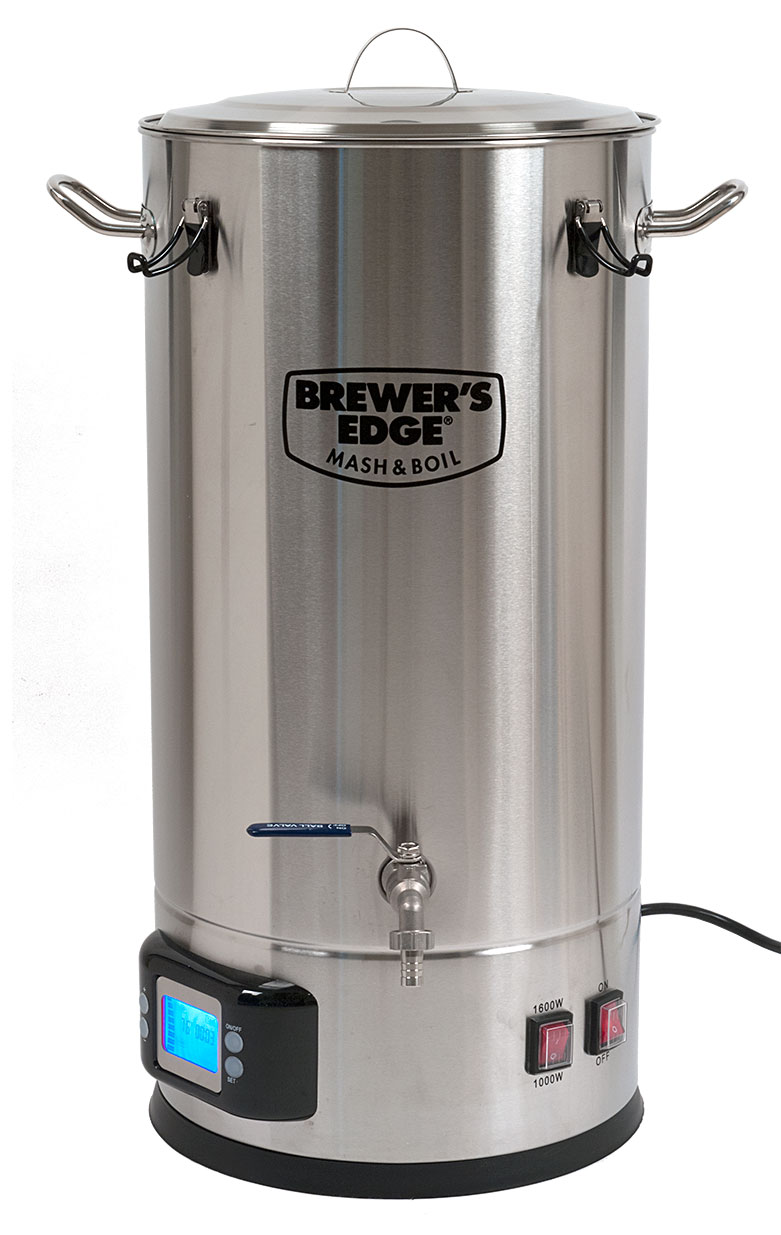
\includegraphics[width=1in]{mashandboil}};
    \node [left of=mashandboil, node distance=1in] (spargewater) {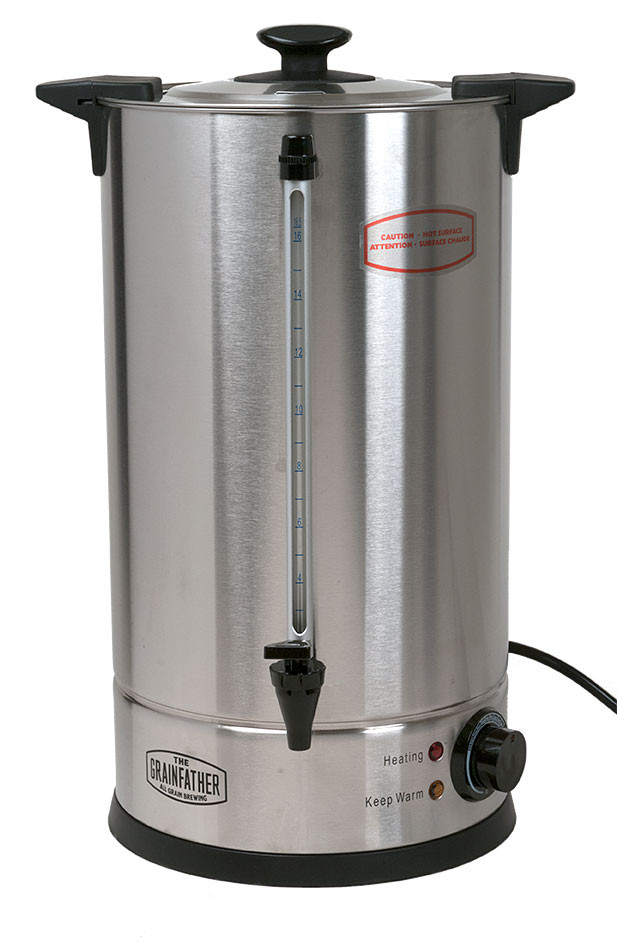
\includegraphics[width=1in]{spargewater}};
    \node [sum,below of=spargewater,node distance=1in] (swout) {};
    \node [sum,above of=mashandboil,node distance=1in] (mbin) {};
    \node [sum,below of=mashandboil,node distance=1in] (mbout) {};
    \node [right of=mbout] (chugger) {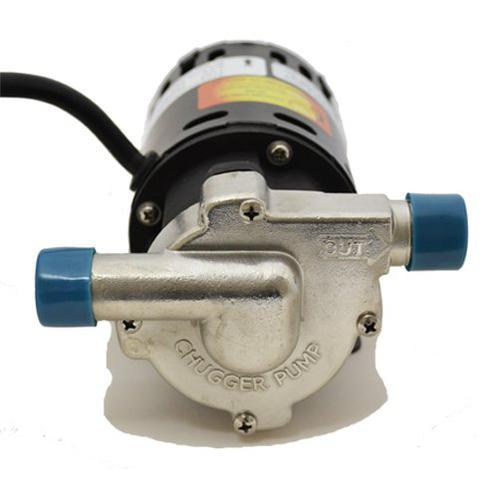
\includegraphics[width=0.5in]{chugger}};
    \node [spdt,above of=chugger,rotate=90] (switch1) {};
    \node [right of=switch1,yshift=0.6cm] (platechiller) {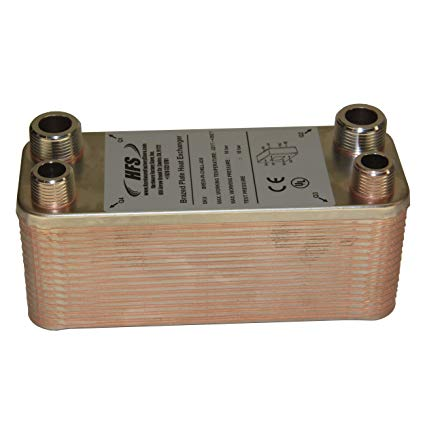
\includegraphics[width=0.5in]{platechiller}};
    \node [above of=platechiller] (tapwater) {Tap Water};
    \node [below of=platechiller] (drain) {Drain};
    \node [output,right of=platechiller] (pcout) {};
    
    % Lines
    \draw (mashandboil) -- (mbin);
    \draw (mashandboil) -- (mbout);
    \draw (spargewater) -- (swout);
    \draw (swout) -- (mbout);
    \draw (mbout) -- (chugger);
    \draw (chugger) -- (switch1.in);
    \draw (switch1.out 1) |- (mbin);
    \draw (switch1.out 2) -| (platechiller.west);
    \draw (platechiller) -- (pcout);
    \draw (platechiller) -- (tapwater);
    \draw (platechiller) -- (drain);
    \draw (pcout) |- (mbin);

    % Annotations
    \node [number] (1)  at (-1.45, 0.3) {1};
    \node [number] (3)  at (-4.0,  0.3) {3};
    \node [number] (4)  at ( 2.3, -3.1) {4};
    \node [number] (5)  at ( 3.1,  0.9) {5};
    \node [number] (10) at (-3.3, -3.0) {10};
    \node [number] (11) at (-1.0,  2.6) {11};
    \node [number] (12) at ( 1.9,  0.5) {12};
\end{tikzpicture}
\caption{Proposed Homebrew Configuration}\label{fig:config}
\end{figure}
\clearpage

Leading up to brew day, do the following\ldots
\begin{enumerate}
    \item Put .3 times the number of pounds in the 
\end{enumerate}
The following is a proposed schedule for brew day using the configuration in Figure~\ref{fig:config}.

\begin{enumerate}
    \item Pour a beer.
    \item Add filtered water to sparge water heater and mash tun.
    \item Set mash tun to heat water to strike water temperature.
    \item Set sparge water heater to boil.
    \item Wait for strike water to come to temperature.
    \item Set flow control valve to bypass plate chiller.
    \item Mash in grain ingredients.
    \item Set timer.
    \item Start pump, and circulate at a slow rate into the top of the grain bed.
    \item Clean primary firmentation bucket, airlock, spoon, scissors, yeast package.
    \item Wait until timer is ended.
    \item Lift the grain tube to upper position.
    \item Close the valve on the mash tun, and open the sparge water valve, slowly sparging with  calculated needed water.
    \item Close the valve on the sparge water heater, remove the grain tube and place in primary firmentation bucket until ready to clean.
    \item Set mash tun to boil temperature.
    \item Add hops as instructed in the recipie.
    \item Clean grain tube.
    \item Set flow control valve to inline plate chiller.
    \item At five minutes left in the boil, leave the tap water valve closed, and open the valve on the mash tun to circulate boiling wort through the plate chiller to sanitize.
    \item Turn off mash tun heating element.
    \item Turn on tap water.
    \item Continue chilling till desired temperature is reached.
    \item Set flow control valve to bypass plate chiller, turn off tap water.
    \item Add yeast.
    \item Let pump circulate to aerate the wort and stir in yeast.
    \item Stop pump.
    \item Move wort aerator to primary firmentation bucket.
    \item Start pump and transfer wort from mash tun to primary firmentation bucket.
    \item Add airlock to primary firmentation bucket.
    \item Remove wort aerator from hose and place hose in drain.
    \item Set flow control valve to inline plate chiller.
    \item Open sparge water heater valve and drain remaining hot water through the plate chiller and into the drain.
    \item Turn off pump.
    \item Disconnect line from sparge water heater and re-connect to compressed air line.
    \item Open compressed air line just enough to purge water from lines, pump, and plate chiller.
    \item Pour another beer.
    \item Clean mash tun.
\end{enumerate}

The plan is to force carbonate in cornelius kegs.
%------------------------------------------------------------------------------
\newday{20181217}

\newentry[Reverse Osmosis Water Collection]{1800 Reverse Osmosis Water Collection}\FloatBarrier{}
In preparation for this Friday's brew day, I will be collecting and storing reverse osmosis filtered water from my kitchen sink system.  The process to filter this water is slow, so each evening I will transfer 1-2 gallons from the filter reservoir to the 5 gallon corny kegs.  On brew day the water in the korny kegs will be transferred to the sparge water heater and mash tun.

%------------------------------------------------------------------------------
\newday{20181220}

\newentry[Grain and Supplies Purchase]{1400 Grain and Supplies Purchase}\FloatBarrier{}
Met with Damon at the Maryland Homebrewers store to purchase grain and supplies.

%------------------------------------------------------------------------------
\newday{20181221}

\newentry[Brew Day]{1000 Brew Day}\FloatBarrier{}
 
%------------------------------------------------------------------------------
\def\todaysdate{20190108}
\newday{\todaysdate}\label{\todaysdate}

\newentry[Racking]{1900 Racking}
\FloatBarrier{}

\begin{my_itemize}
    \item Assembled the new transfer pump.  I cut the supplied hose in half, and attached one side of each half to the pump, then the source side to the stainless steel racking cane, and the other side to a beer side ball lock connector.
    \item A gas side ball lock disconnect with no fittings was attached to the other post to allow air to vent.
    \item I attached the ball lock to the target cornelius keg, and inserted the racking cane into a gallon milk jug filled with sanitizer.  I pumped several cups of water into the cornelius keg, and then shook the cornelius keg making sure the sanitizer was splashed against all sides of the keg.  I let the solution sit for two minutes, then opened the keg and poured out the sanitizer, and pumped out the remaining sanitizer in the lines.  I then opened the primary fermentation bucket inserted the racking cane about an inch below the surface, and started the pump.  As I neared the bottom I tilted the bucket to get the last bit.
    \item The beer has a nice dark color, and there was sign of a good amount of krausen on the sides of the bucket but not on the beer.  The layer of trub was about 1/2 inch thick.
    \item The content of the bucket was slightly more than the capacity of the keg, and a bit sprayed out of the vent at the end across my basement.  A future improvement could be to add a hose to the air vent and drop it into a bucket in case of overflows.
\end{my_itemize}

\begin{figure}[H]
  \centering
  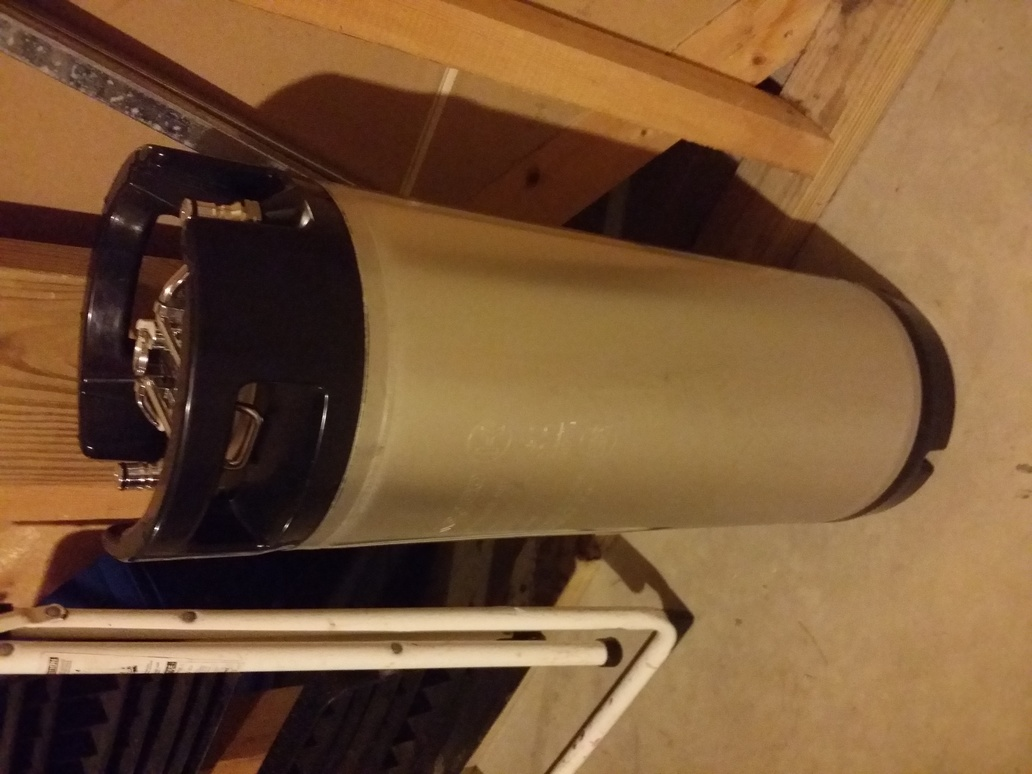
\includegraphics[angle=270,origin=c,width=0.5\textwidth]{IMG_20190108_195458_reduced}
  \caption{Force Carbonation}\label{fig:racking:complete}
\end{figure}

\begin{figure}[H]
  \centering
  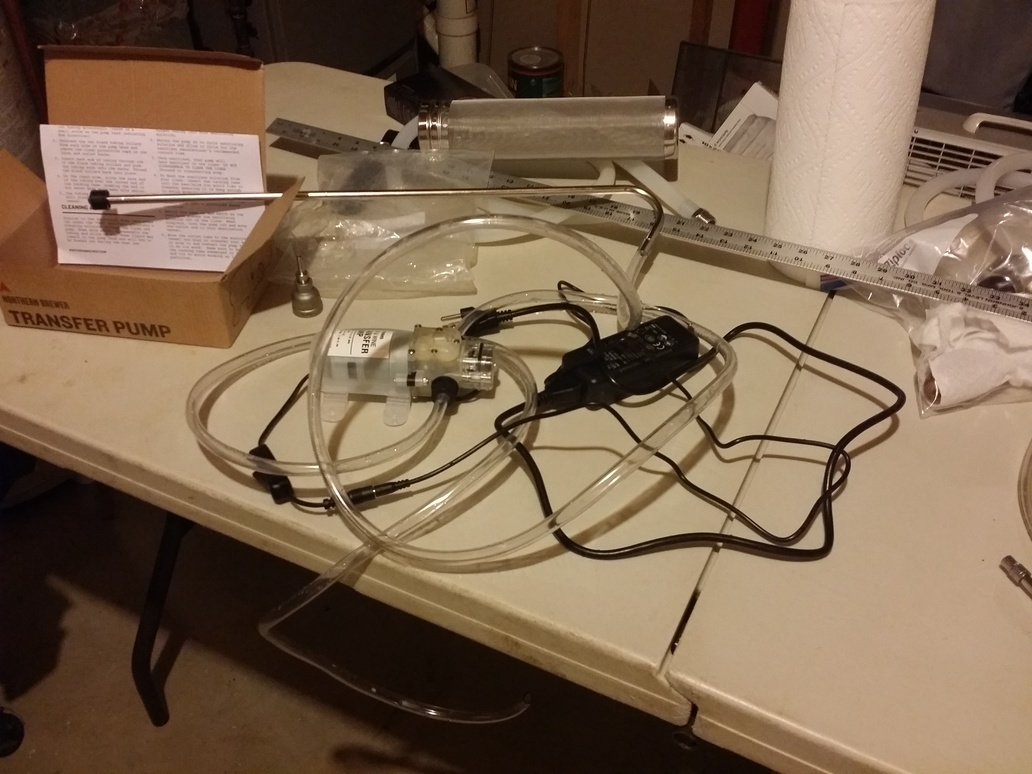
\includegraphics[angle=0,origin=c,width=\textwidth]{IMG_20190108_195511_reduced}
  \caption{Force Carbonation}\label{fig:racking:transferpump}
\end{figure}

\FloatBarrier{}
\clearpage
%------------------------------------------------------------------------------
\def\todaysdate{20190111}
\newday{\todaysdate}\label{\todaysdate}

\newentry[Beginning Force Carbonation]{1900 Beginning Force Carbonation}
\FloatBarrier{}

\begin{my_itemize}
    \item Assembled the force carbonization hardware.
    \item I swapped out the regulator on my kegerator for the new one I bought for force carbonating.  The one on my kegerator was very difficult to keep dialied into a setting.  The new regulator seems to be of a much higher quality.  I will put the better regulator on the serving system, the kegerator, and use the lesser regulator to force carbonate.
    \item A CO2 hose was attached to the regulator's hose barb, which was a 5/16'' barb, and to the barb on the gas ball lock disconnect.  The barb on the gas ball lock was only a 1/4'', so I wrapped several layers of silicone tape over the barb before inserting it into the hose.  I also used two clamps on this side of the hose.  This provided an airtight seal.
    \item The ball lock was attached to the corny keg, and the pressure release valve was pulled several times to make sure the air was purged from the keg and that only CO2 remained.  The pressure on the CO2 regulator was left at 10psi.
\end{my_itemize}

\begin{figure}[H]
  \centering
  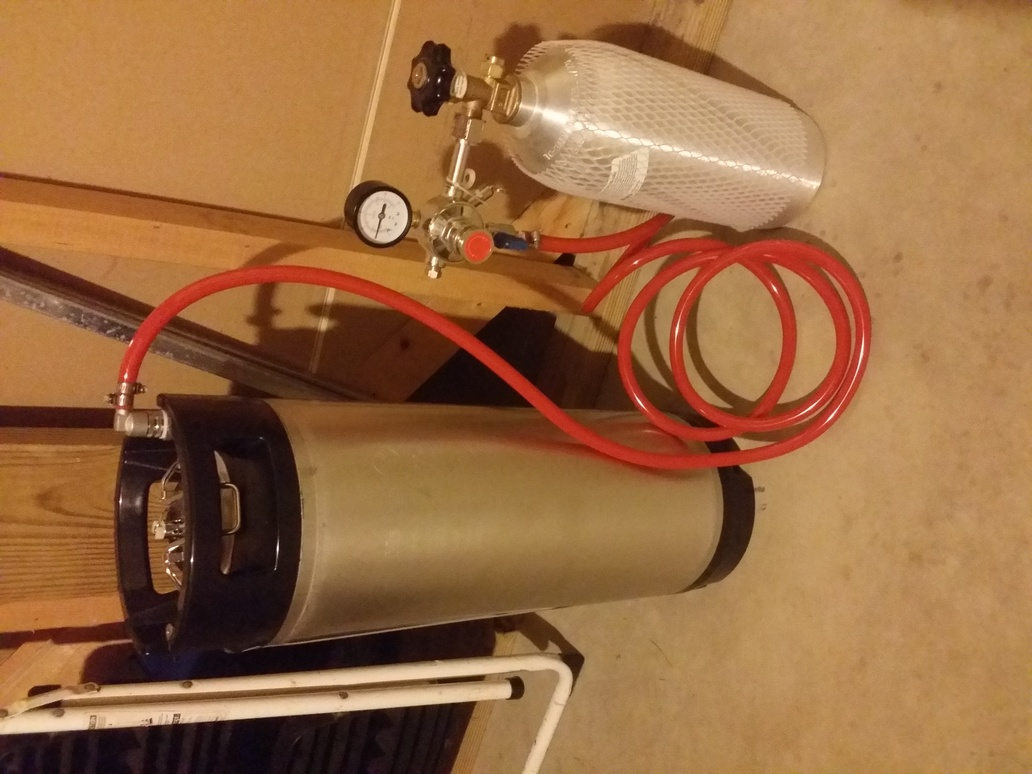
\includegraphics[angle=270,origin=c,width=0.5\textwidth]{IMG_20190111_212159_reduced}
  \caption{Force Carbonation}\label{fig:forcecarbonation}
\end{figure}

\FloatBarrier{}
\clearpage

%------------------------------------------------------------------------------
\def\todaysdate{20190111}
\newday{\todaysdate}\label{\todaysdate}

\newentry[Sample]{1900 Sample}
\FloatBarrier{}

A faucet was installed on the beer post with a quick connect adapter.  The faucet is a perlick.  For future reference, perlicks are wonderful faucets, but there is no spring loaded close off of the valve.  When I attached the faucet, the keg was under pressure, and the valve was open.  So another spill occurred in the basement, shown in figure~\ref{fig:sample:mishap}.  After a few minutes of cleaning up concrete, I was able to draw a sample.

Figures~\ref{fig:sample:1} and~\ref{fig:sample:2} show the sample that was drawn.  Tasting shows no ``off'' flavors.  That is, no hints of milk, apple, cardboard, or anything else other than a subtly hopped dark but a bit flat beer.

The faucet was removed from the keg, and the CO\textsubscript{2}, and the keg was installed in the kegerator upstairs to just the CO\textsubscript{2} line.  I want to clean the beer lines before connecting to this new keg as the kegerator has been empty, but refridgerated for over a month.  The temperature was dialed in at 42 degrees, and the pressure set for 20psi.  After two days at this temperature and pressure, I plan to dial the pressure down to 10psi.

Funny Story:  My kids got a google mini for Christmas, and when they are board, have been playing with the new features.  It just happens they had it sitting on top of my kegerator because there was a power outlet near by, and it just happened that the kids were playing with their tablet in the other room just as I finished installing the keg.  So right after I install the keg, and close the door to the kegerator, the kegerator says to me ``I love you daddy!''.  They had just discovered the ``broadcast a voice message'' feature.

\begin{figure}[H]
  \centering
  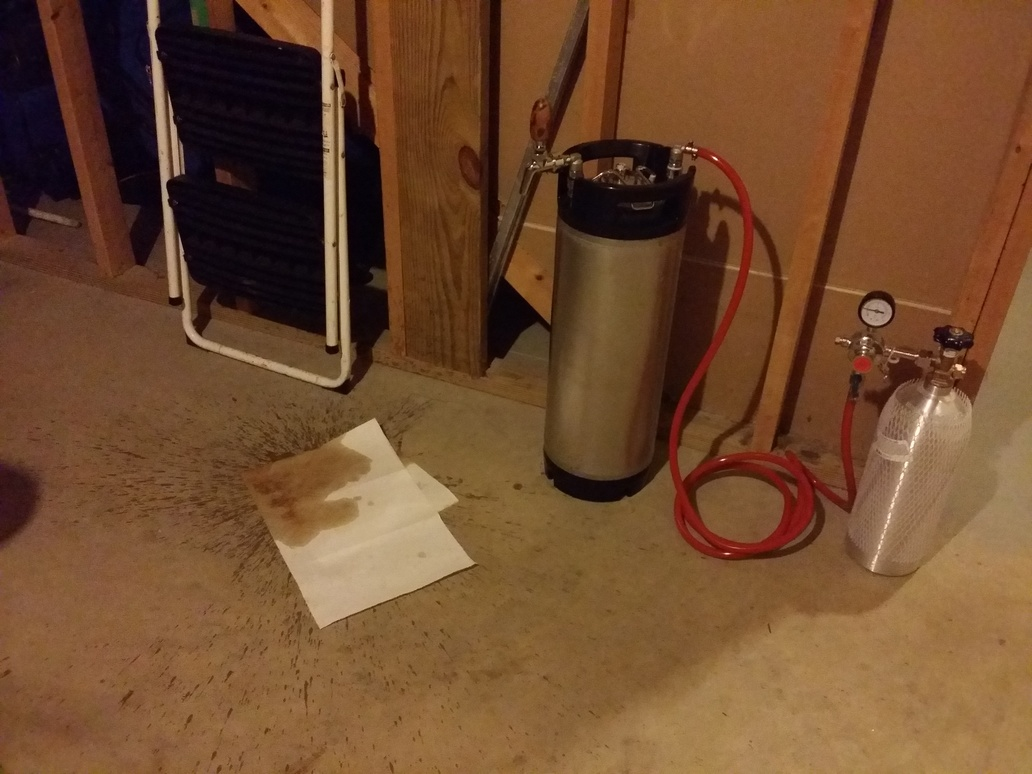
\includegraphics[angle=0,origin=c,width=\textwidth]{IMG_20190114_182953_reduced}
  \caption{Sample mishap}\label{fig:sample:mishap}
\end{figure}

\begin{figure}[H]
\begin{minipage}{0.45\textwidth}
  \centering
  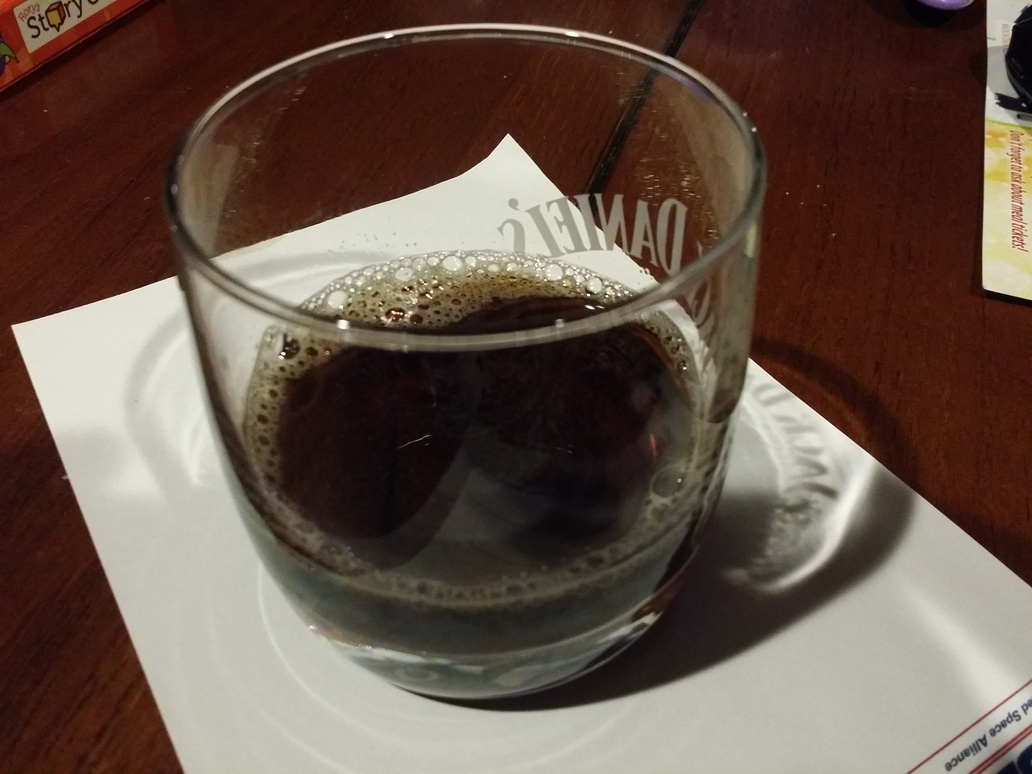
\includegraphics[width=\textwidth]{IMG_20190114_183506_reduced}
  \caption{Sample View 1}\label{fig:sample:1}
\end{minipage}\hfill
\begin{minipage}{0.45\textwidth}
  \centering
  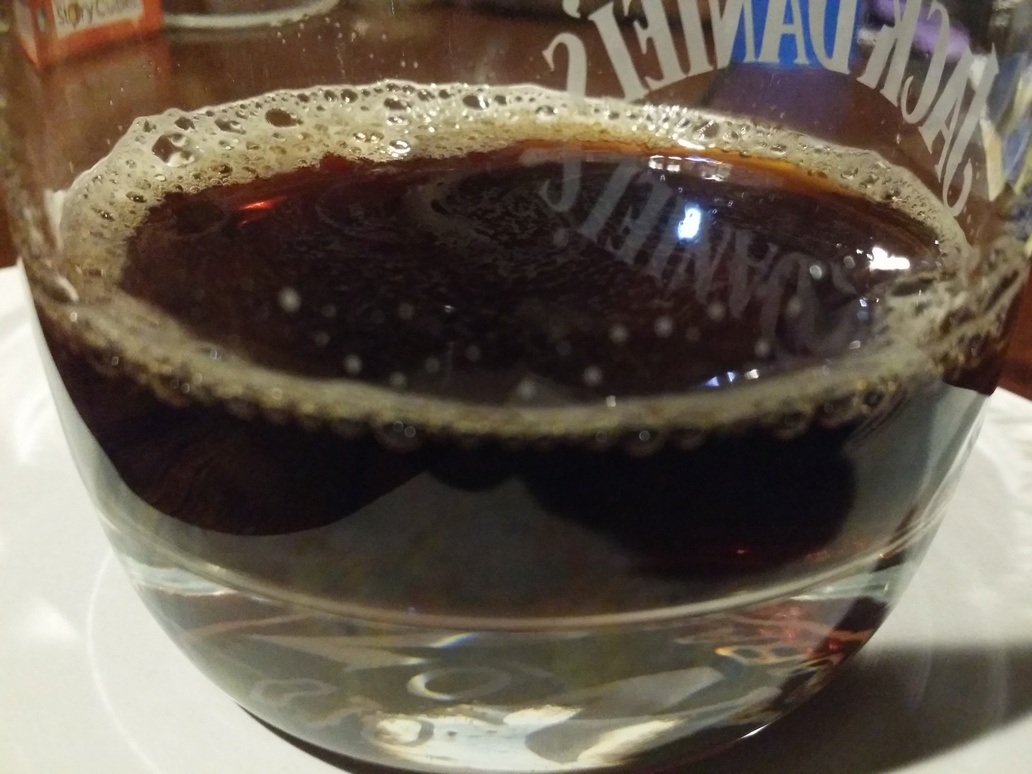
\includegraphics[width=\textwidth]{IMG_20190114_183526_reduced}
  \caption{Sample View 2}\label{fig:sample:2}
\end{minipage}
\end{figure}

\FloatBarrier{}
\clearpage

\begin{figure}[H]
  \centering
  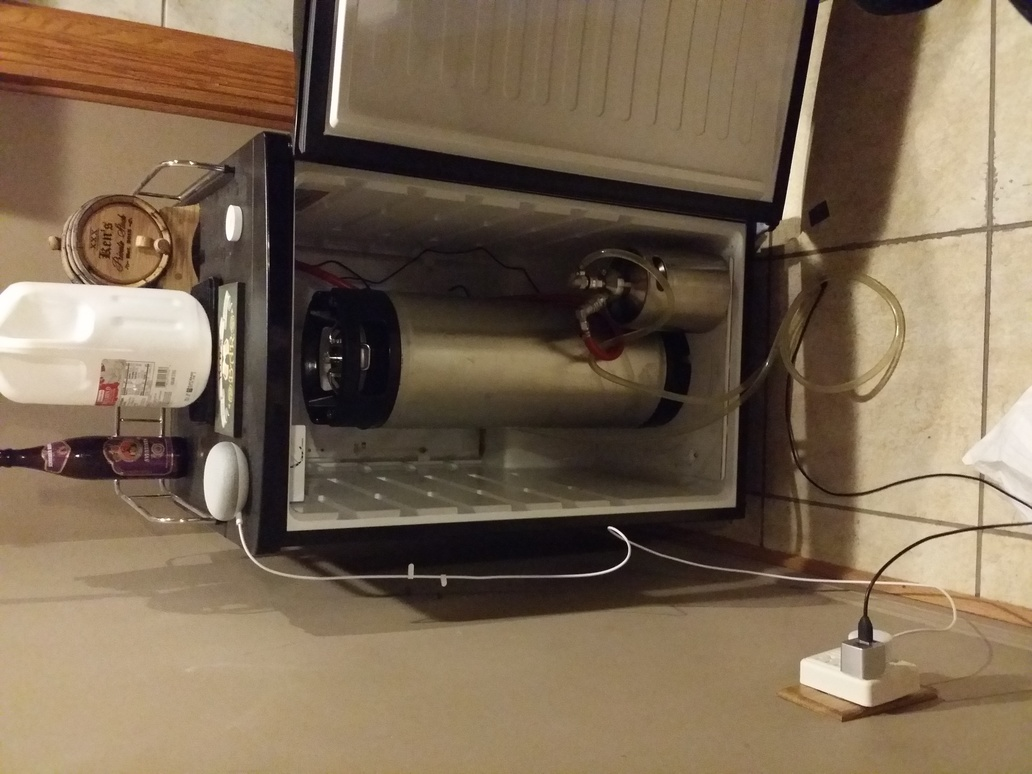
\includegraphics[angle=270,origin=c,width=0.5\textwidth]{IMG_20190115_204926_reduced}
  \caption{Cleaning kegerator lines}\label{fig:cleaning}
\end{figure}

\begin{figure}[H]
  \centering
  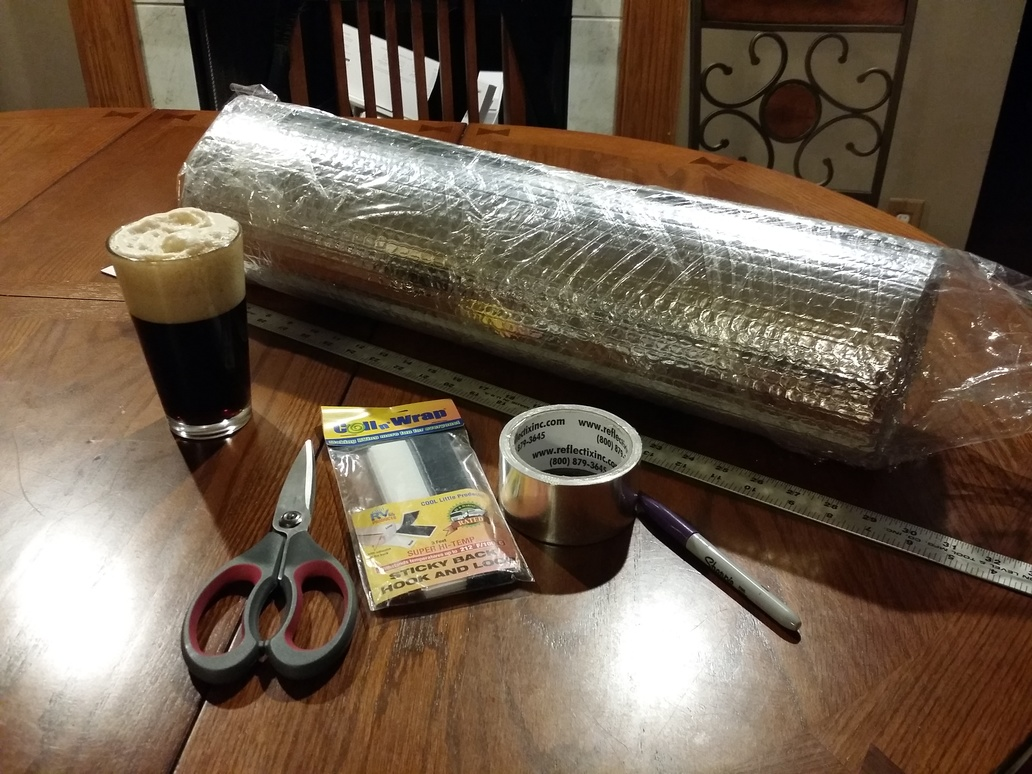
\includegraphics[width=\textwidth]{IMG_20190119_172654_reduced}
  \caption{Preparing to make brew jacket}\label{fig:brewjacket:prep}
\end{figure}

\begin{figure}[H]
  \centering
  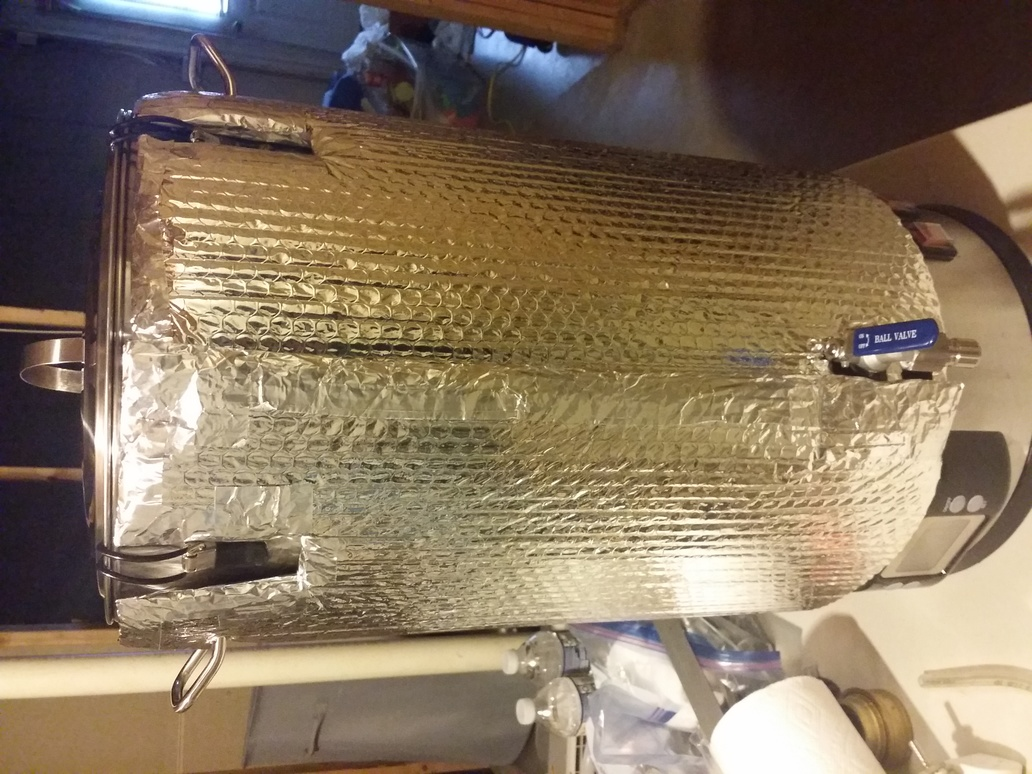
\includegraphics[angle=270,origin=c,width=0.5\textwidth]{IMG_20190120_121041_reduced}
  \caption{Completed Brew Jacket Side View}\label{fig:brewjacket:side}
\end{figure}

\begin{figure}[H]
  \centering
  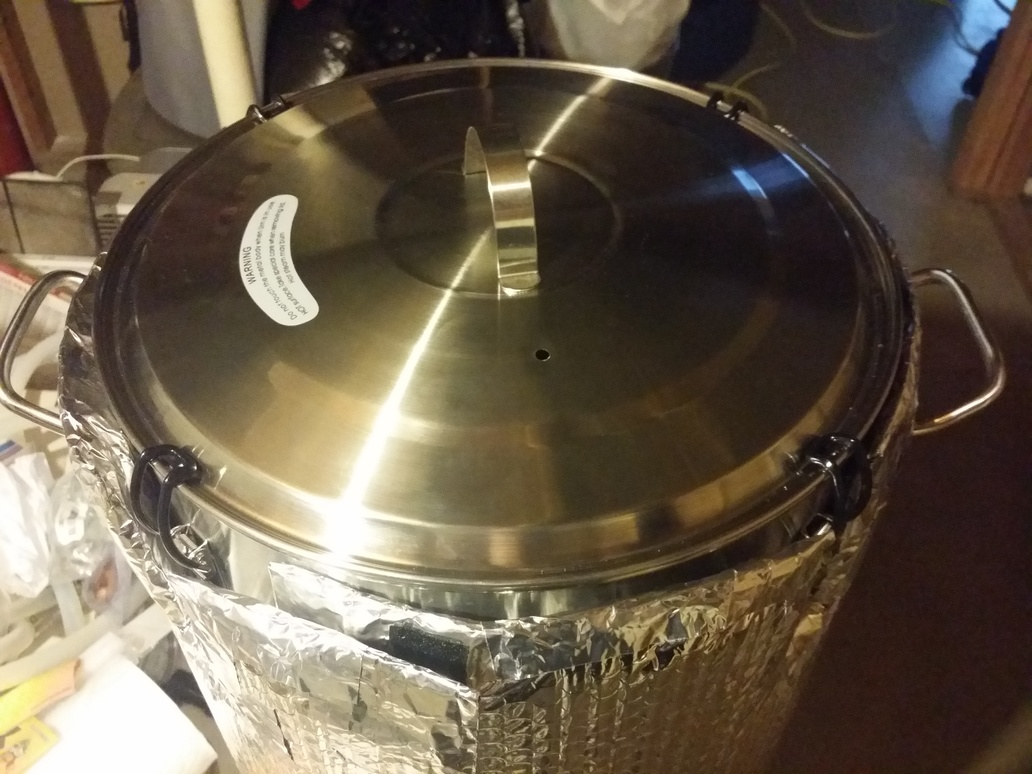
\includegraphics[width=\textwidth]{IMG_20190120_121055_reduced}
  \caption{Completed Brew Jacket Top View}\label{fig:brewjacket:top}
\end{figure}

\begin{figure}[H]
  \centering
  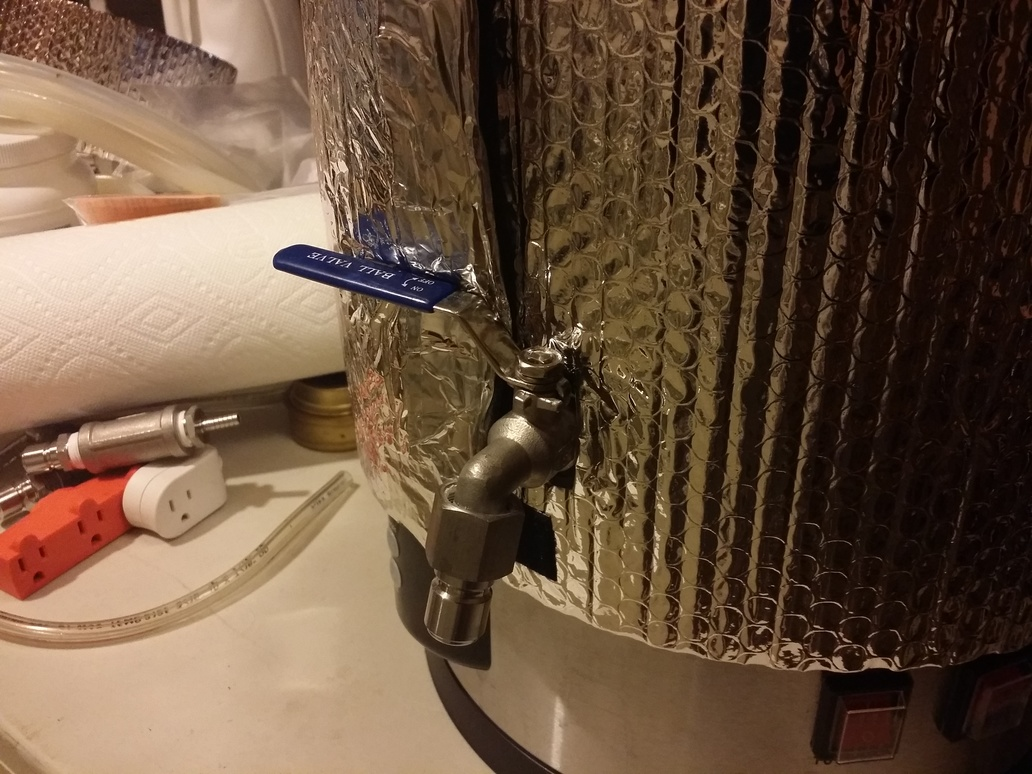
\includegraphics[width=\textwidth]{IMG_20190120_121114_reduced}
  \caption{Completed Brew Jacket Valve Closeup}\label{fig:brewjacket:valve}
\end{figure}

%------------------------------------------------------------------------------
\def\todaysdate{20190126}
\newday{\todaysdate}\label{\todaysdate}

\newentry[Brew]{0754 Brew}
\FloatBarrier{}
1721 Mixed up a gallon of sanitizer.  One step, 1 tbsp.

1725 Added 4.5 gallons to mash tun as read by the markers on the inside of the mash tun, set to heat to 173

1736 Placed air trap and yeast in sanitizer in bowl, set aside

1742 Sanitized a small piece of beer tube.  Will place this between filter and stone in aerator.

1744 Sprayed everclear into aeration stone

1803 Added Added just short of to the 13 L mark water to the sparge water heater, and turned on the heat

1807 Drank a beer from the last batch

1823 Mash Tun water temp reached 173, Beginning Mash in

1833 Mash in complete, temp is 164, leaving lid off of top to allow heat to escape

1837 Temp is down to 162

1845 Temp is down to 158

1856 Temp is down to 154 Placed lid back on mash tun

1904 Temp is 152

1921 Temp is 148 (Note Warmer kicks in at 6 degrees below set temperature)

1933 Lifted basket, started recirculating wort, set heater to 165

1943 Shut off pump and closed valve on mash tun, started pump, and opened valve on sparge water heater, watching for 10.4 L of water to transfer  Note the white line between 75 and 80 on the sparge water heater seems to correspond to the correct sparge water temperature.

2019 10.4 L of water completed transfer to top.  I tried to maintain about one inch of water over the grain bed, it was pretty easy to dial in the speed to do that, ask damon later if the full hour should be spent transferring sparge water or if it is ok to sparge for 30 minutes, then drain for 30 minutes.  Note, there is still a slow leak on the sparge water faucet, it is coming out between the quick connect and the spicot

2034 Leak started to get worse.  Used some X-TREME tape on the connection, and the leak has stopped.

2043 Set heater to 220.  Note: Since it takes a while to get to boil, I should have started the heater at 30 minutes into sparge, the sparging basket could have completed draining while the water was coming up to temperature.

2050 Removed sparging basket.  Wort level is at 6 Gallon mark on mash tun

2113 214 degrees reached according to mash tun, 1 hour timer started, adding challenger hops in hop spider.  While opening the hops, the kettle almost boiled over.  The hop spyder when placed in cut down the foam almost instantly.

2145 Drinking Beer

-15 Added irish moss

-5 Added willamette and turned on pump, temperature dropped to 203 and boil has stopped

2230 Yeast pitched, stirred, tilt was added after sitting in sanitizer for 10 minutes, and the airlock was installed and filled.  Ended up with about 5.15 gallons of wort, with 1.050 OG

01/27/2019
0101 Done Cleaning

\begin{figure}[H]
  \centering
  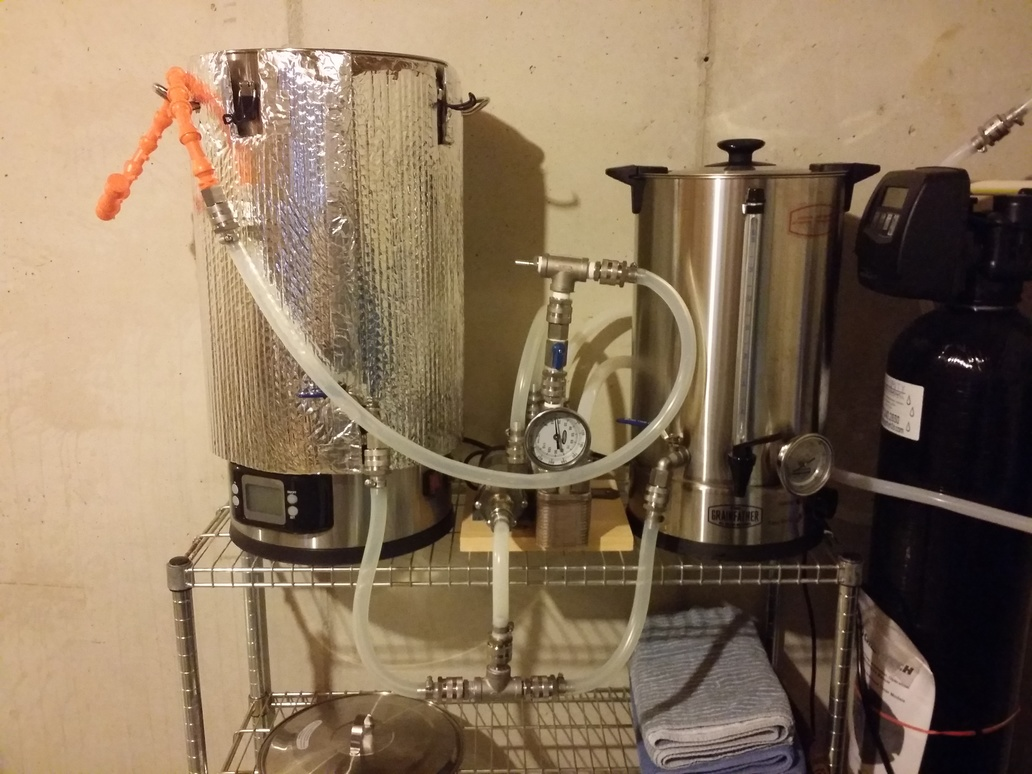
\includegraphics[width=\textwidth]{IMG_20190126_081006_reduced}
  \caption{Setting up for Brew}\label{fig:brew:setup}
\end{figure}

\begin{figure}[H]
  \centering
  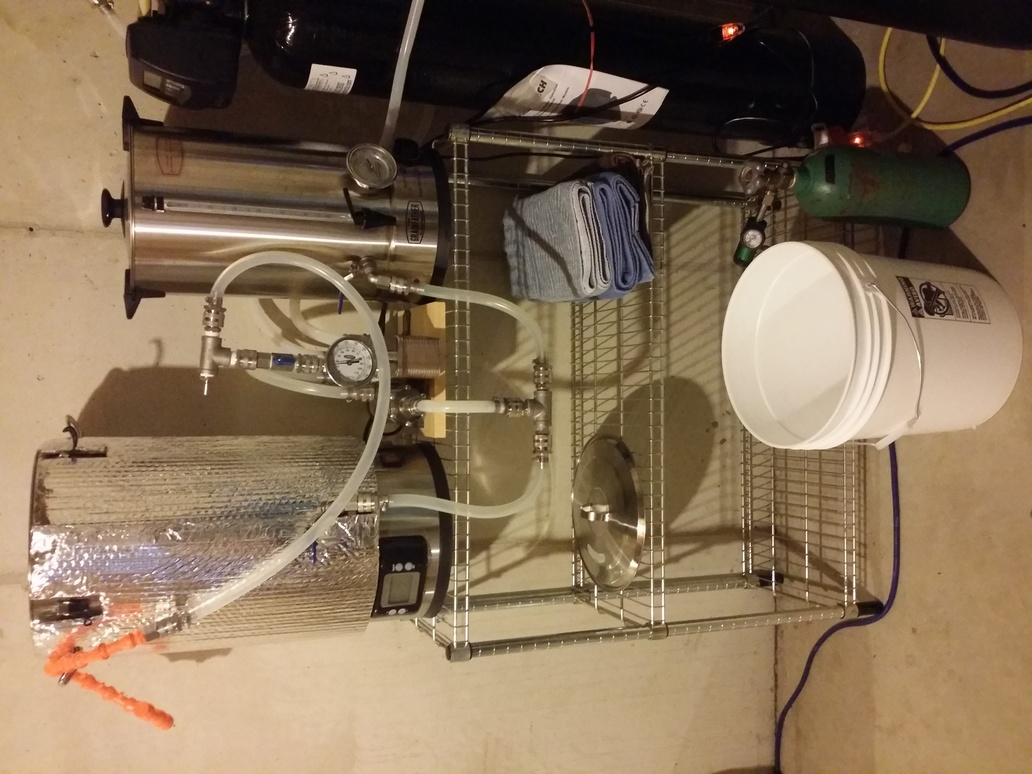
\includegraphics[angle=270,origin=c,width=0.5\textwidth]{IMG_20190126_081031_reduced}
  \caption{Setting up for Brew}\label{fig:brew:setup2}
\end{figure}

\begin{figure}[H]
  \centering
  \includegraphics[width=\textwidth]{IMG_20190126_182020_reduced}
  \caption{Setting up for Brew}\label{fig:brew:setup3}
\end{figure}

\begin{figure}[H]
  \centering
  \includegraphics[angle=270,origin=c,width=0.5\textwidth]{IMG_20190126_190856_reduced}
  \caption{Brew Receipt}\label{fig:brew:receipt}
\end{figure}

\begin{figure}[H]
  \centering
  \includegraphics[angle=270,origin=c,width=0.5\textwidth]{IMG_20190126_191149_reduced}
  \caption{Brew Receipt}\label{fig:brew:receipt}
\end{figure}

\begin{figure}[H]
  \centering
  \includegraphics[angle=270,origin=c,width=0.5\textwidth]{IMG_20190126_195156_reduced}
  \caption{Sparging}\label{fig:brew:sparge}
\end{figure}

\begin{figure}[H]
  \centering
  \includegraphics[angle=270,origin=c,width=0.5\textwidth]{IMG_20190126_203251_reduced}
  \caption{Patch for leak}\label{fig:brew:leak}
\end{figure}

\begin{figure}[H]
  \centering
  \includegraphics[width=\textwidth]{IMG_20190126_211535_reduced}
  \caption{Hop Additions}\label{fig:brew:hopadditions}
\end{figure}

\begin{figure}[H]
  \centering
  \includegraphics[angle=270,origin=c,width=0.5\textwidth]{IMG_20190126_222126_reduced}
  \caption{Chilling and transfer to Primary Fermentation}\label{fig:brew:chilling}
\end{figure}

\begin{figure}[H]
  \centering
  \includegraphics[angle=270,origin=c,width=0.5\textwidth]{IMG_20190126_222143_reduced}
  \caption{Temperature Exiting Plate Chiller}\label{fig:brew:chilltemp}
\end{figure}

\begin{figure}[H]
  \centering
  \includegraphics[width=\textwidth]{IMG_20190127_080524_reduced}
  \caption{Sediment at bottom of empty keg}\label{fig:keg1:empty}
\end{figure}

\begin{figure}[H]
  \centering
  \includegraphics[angle=270,origin=c,width=0.5\textwidth]{IMG_20190208_185003_reduced}
  \caption{Receipt}\label{fig:brew:receipt}
\end{figure}

%------------------------------------------------------------------------------
\def\todaysdate{20190209}
\newday{\todaysdate}\label{\todaysdate}

\newentry[Brew]{0754 Brew}
\FloatBarrier{}
0754 Start Heating water.  Filled to 4.5 gallon mark on mash tun, set temperature to 163.  Put 13.5 liters in the sparge water heater, and started heat

0759 Mixed one gallon of one step cleaner/sanitizer

0845 Water is up to 163 in the mash tun. Reduced temperature setting of mash tun to 152, starting mash in

0855 Ended Mash In, temperature at 160.  Reduced temperature setting of mash tun to 152.  Note: I would have been closer to the 152 target if I had lowered the temperature setting before mash in.  I noticed when I was done mashing in the heater had been running the whole 10 minutes.  Leaving lid off to let temperature drop to target temp faster.

0938 Mash tun temp down to 152, placed lid back on

0955 Raised mash tube up, started pump at slow pace to recirculate wort

1025 Starged sparging, targeting 8L of water for sparging, turned on heater to start getting up to boil temperature

Note:  Sparging slow as I should, I am taking too long, for recirculating for 30 minutes.  Next time recirculate for only 10 minutes after raising the mash tube.

Note:  Sparge water in tank reads 168, exiting the plate chiller at 158, and going into the mash tube at 148

1118 8 Liters completed sparging, letting wort finish draining from grain bed.

Note: New strategy, recirculate 10 minutes, sparge 50-60, and end of sparge, turn on heater to 220, and let the mash tube sit on top until boil is reached.

1149 Removed grain bed, wort level is just below the 5.5 gal mark on the mash tun

1200 Boil started, added challenger hops in hop spider

1245 Added 1 teaspoon irish moss

\begin{figure}[H]
  \centering
  \includegraphics[angle=270,origin=c,width=0.5\textwidth]{IMG_20190209_082312_reduced}
  \caption{Setting up for brew}\label{fig:brew:setup}
\end{figure}

\begin{figure}[H]
  \centering
  \includegraphics[angle=270,origin=c,width=0.5\textwidth]{IMG_20190209_101016_reduced}
  \caption{Sparging}\label{fig:brew:sparge}
\end{figure}

\begin{figure}[H]
  \centering
  \includegraphics[width=\textwidth]{IMG_20190209_131702_reduced}
  \caption{Aeration Complete}\label{fig:brew:aeration}
\end{figure}

\begin{figure}[H]
  \centering
  \includegraphics[angle=270,origin=c,width=0.5\textwidth]{IMG_20190213_212835_reduced}
  \caption{Sample Pour}\label{fig:sample:pour}
\end{figure}

\begin{figure}[H]
  \centering
  \includegraphics[width=\textwidth]{IMG_20190223_190343_reduced}
  \caption{Juice for Cider}\label{fig:brew:juice}
\end{figure}

\begin{figure}[H]
  \centering
  \includegraphics[width=\textwidth]{IMG_20190223_190405_reduced}
  \caption{Sanitizing for Cider}\label{fig:brew:sanitizing}
\end{figure}

\begin{figure}[H]
  \centering
  \includegraphics[width=\textwidth]{IMG_20190223_190424_reduced}
  \caption{Brown Sugar for Cider}\label{fig:brew:brownsugar}
\end{figure}

\begin{figure}[H]
  \centering
  \includegraphics[angle=270,origin=c,width=0.5\textwidth]{IMG_20190223_194644_reduced}
  \caption{Beginnign of Primary Fermentation}\label{fig:brew:primary}
\end{figure}

\begin{figure}[H]
  \centering
  \includegraphics[width=\textwidth]{IMG_20190225_171122_reduced}
  \caption{Sediment at Empty Keg}\label{fig:keg2:empty}
\end{figure}

\begin{figure}[H]
  \centering
  \includegraphics[width=\textwidth]{IMG_20190305_090133_reduced}
  \caption{Sediment at Empty Keg}\label{fig:keg3:empty}
\end{figure}

\begin{figure}[H]
  \centering
  \includegraphics[angle=270,origin=c,width=0.5\textwidth]{IMG_20190315_181311_reduced}
  \caption{Receipt}\label{fig:brew:receipt}
\end{figure}

%------------------------------------------------------------------------------
\def\todaysdate{20190317}
\newday{\todaysdate}\label{\todaysdate}

\newentry[Brew]{0700 Brew}
0700 Placed 4 gallons in mash tun and set heater to 130, 5 gallons in sparge water heater
0728 Set mash tun temperature to 120 and began mash in
0834 Mash in complete, beginning 20 minute protein rest, mash temp at 119
0835 Set mash tun temperature to 110 as re-inspection of the recipie listed 110
0854 Increased temperature to 152 and began slow recirculation
0916 152 degrees in mash tun, starting 1 hour mash with slow recirculation continuing
1016 Raised grain tube, set the heater to 168, and continued reciculating for 10 minutes.
1026 Closed valve on the mash tun and opened the valve on the sparge water heater.  Targeting 11L of sparge water.
1044 13L of sparge water transferred, turned off pump and closed the valve on the sparge water.  Set the mash tun temperature to 220.
1112 Collected enough wort to fill up to the 5.5 gallon mark on the mash tun.  Removed the mash tube, and placed empty hop spider into the wort to break the surface tension at boil.
1114 Boil started, began 30 minute timer for hop addition
1145 Added hops to hop spider
1240 Started Recirculating water to sanitize the pump and hose
1245 Turned off heat to the mash tun, tuned on water flow to the plate chiller, slowed flow till water temperature reading exiting the plate chiller was mid to low 60's, then turned on the oxygen and started transfer to the primary fermentation bucket.
1529 Done cleaning.

Note: Sparge heater set to 80 for sparging, set to 65 for warming cleaning water.
Note: Next time, remember to spray sanitizer in the oxygen fittings and stone, if there is an infection during fermentation, this is the vector.

%------------------------------------------------------------------------------
\def\todaysdate{20190324}
\newday{\todaysdate}\label{\todaysdate}

\newentry[Brew]{0730 Brew}
0730 Placed 4.5 gallons in mash tun and set heater to 162.  Connected all hoses, bags, and mixed one gallon of sanitizer.  Yeast packet was placed in tupperware with sanitizer along with the airtrap and the scissors.
0820 Set the mash tun temperature to 154 and began mash in
0830 Mash in complete, circulationi started, at the end of mash in temp is 159.
Note:  The check valve and cutoff for the oxygen was placed in the sanitizer solution, but a reaction occurred with the metal in the valve shutoff handle.  Everything in the sanitization solution was cleaned off, and a new sanitizer bath was poured and the check valve was sanitized again, but this time with alcohol.
0930 Raised temperature setting to 168
0940 Raised mash tube, continued recirculating wort
0950 Closed valve on the mash tun and opened the valve on the sparge water heater.  Targeting 11L of sparge water.
1127 11L of sparge water transferred, turned off pump and closed the valve on the sparge water.  Set the mash tun temperature to 220.
1200 Boil started, began 30 minute timer for hop addition
1230 Added hops to hop spider
1325 Started Recirculating water to sanitize the pump and hose
 Turned off heat to the mash tun, tuned on water flow to the plate chiller, slowed flow till water temperature reading exiting the plate chiller was mid to low 60's, then turned on the oxygen and started transfer to the primary fermentation bucket.
 Done cleaning.

%------------------------------------------------------------------------------
\def\todaysdate{20190511}
\newday{\todaysdate}\label{\todaysdate}

\newentry[Brew]{0710 Brew}
Startup Notes.
\begin{my_itemize}
  \item The mash tun was filled with exactly 4 measured gallons of water.  The water line in the mash tun came up half a gallon below the 4 gallon mark.  One half gallon was added, and the water level was exactly at 4 gallons.  The water was drained out, and the dead space at the bottom of the mash tun below the valve was just a little less than half a gallon.  Their lines must not account for the dead space.  To start with 4.5 gallons of water, water needs to be filled to the 4 gallon mark in the mash tun.
  \item The chapman stainless steel fermentation buckets are about a quarter gallon off.  Two gallons of water reads about 1.75 on the gradations on the bucket.
\end{my_itemize}
0710 Start 4.5 Gallon in mash tun at 160
0750 Reached Temp
0810 Set mash tun to 154 deg, started Mash In
0820 Mash in complete temp at 148
0920 Raised temperature setting to 168
0930 Raised mash tube, Closed valve on the mash tun and opened the valve on the sparge water heater.  Targeting 11L of sparge water.
1026 10L of sparge water transferred, turned off pump and closed the valve on the sparge water.  Set the mash tun temperature to 220.
1100 While heating up to boiling, another 5L of water was added to adjust the gravity the refractometer read 1.048 
1110 Boil Started
1250 Begin Transfer

1330 Start 4.5 Gallon in mash tun at 161
1400 Reached Temp
1415 Set mash tun to 154 deg, started Mash In
1420 Mash in complete temp at 154
1520 Raised temperature setting to 168
1530 Raised mash tube, Closed valve on the mash tun and opened the valve on the sparge water heater.  Targeting 11L of sparge water.
1620 11L of sparge water transferred, turned off pump and closed the valve on the sparge water.  Set the mash tun temperature to 220.
1647 Boil Started SG 1.041
0710 Finished Cleaning

%------------------------------------------------------------------------------
\def\todaysdate{20190706}
\newday{\todaysdate}\label{\todaysdate}

\newentry[Brew]{0710 Brew}

Original Recipe

\begin{verbatim}
Schneider Weisse Aventinus tap 6 clone

5000g wheat malt
2000g Munich malt EBC 20
1000 Caramunch malt EBC 50
2000g Pilsner malt

Stepped mash:
30 minutes@50C in 15litres
Protein rest with grist/ liquor ratio 1:1.15
Raise to 65c for 60 mins with 8litres @ 100c
Sparge @72C to collect 25 litres wort.

Boil:
40g Hallertau Herbrucker@70 mins
10 g H H @ 15 mins
5g Irish Moss @15

Collected 18 litres.
Wyeast 3068 Weihenstephan Weizen
OG 1058
FG 1016
\end{verbatim}

\begin{description}
    \item[5000g] Wheat Malt
    \item[2000g] Munich Malt
    \item[2000g] Pilsner Malt
    \item[1000g] Caramunich Malt
\end{description}

Stepped Mash
\begin{enumerate}
  \item 30 Minutes at 120$^{\circ}$F in 4 gallons of liquor.
  \item Raise to 150$^{\circ}$ for 60 Minutes
  \item Sparge
\end{enumerate}

Boil
\begin{enumerate}
    \item Boil 90 Minutes
    \item 40g Hallertau Hersbrucker (4\% alpha acids): -70 Minutes
    \item 10g Hallertau Hersbrucker (4\% alpha acids): -15 Minutes
    \item 5g Irish Moss: -15 Minutes
\end{enumerate}

Target OG: 1.058
Target FG: 1.016

%------------------------------------------------------------------------------
\def\todaysdate{20190707}
\newday{\todaysdate}\label{\todaysdate}

\newentry[Brew]{1100 Brew}
Brewing Cider

\begin{itemize}
    \item Boiled .75 gallons of applejuice with 7 lbs of light brown sugar.
    \item Sanitized lids of applejuice, fermentation bucket, air trap, tilt sensor, and scissors.
    \item While bringing brown sugar and apple juice to a boil, the fermentation bucket was filled with the remainder of apple juice and the blender attachment was run to oxygenate the juice.
    \item The brown sugar and juice mixture was boiled for 5 minutes, then poured into the fermentation bucket.
    \item The resulting temperature in the fermentation bucket was 75 degrees, which was safe for the yeast, so the yeast was pitched, and then the blender was used for 10 minutes to continue oxygenating the mixture.
    \item The tilt sensor was added to the bucket, and the lid was secured and air lock filled with sanitizer.
    \item The fermentation bucket was placed in the kegerator at 68 degrees.
\end{itemize}

%------------------------------------------------------------------------------
\def\todaysdate{20190710}
\newday{\todaysdate}\label{\todaysdate}

\newentry[Inventory]{1700 Loading Inventory}
\FloatBarrier{}
1. Munich Malt Lite
2. Pilsen Malt
3. Caramunich (5/29/19)
4. Wheat Malt

\newentry[Brew]{1730 Brew}
\FloatBarrier{}
1730 Start Heating water.  Filled to 4.0 gallon mark on mash tun, which equates to 4.5 gallons of water, set temperature to 160.  Put 13.5 liters in the sparge water heater, and started heat

1815 Water is up to 162 in the mash tun. Reduced temperature setting of mash tun to 152, starting mash in

1820 Ended Mash In, temperature at 151.  Starting recirculation.

1920 Raised mash tube up. Starged sparging, targeting 7.5L of water for sparging over approximately an hour.  Setting temperature of kettle to 170.

2018 7.5 Liters completed sparging, letting wort finish draining from grain bed.  Set the kettle temperature to 220 to bring the wort to a boil.

2049 Removed grain bed, wort level is just below the 5.5 gal mark on the mash tun

2053 Boil started, added challenger hops 1oz 7.8\% in hop spider.  Collected just under the 5 gallon mark on kettle, which is 5.45 gallons or so.  Gravity at Boil is: 1.048

2138 Added 1 teaspoon irish moss

2148 Added 1oz Willamette 4.2\%

2153 Boil Complete.  Trasfer to primary fermentation bucket with yeast at 66 degrees.

Target OG: 1.050
Target Temperature: 66F

%------------------------------------------------------------------------------
\def\todaysdate{20190807}
\newday{\todaysdate}\label{\todaysdate}

\newentry[Brew]{1630 Brew}
\FloatBarrier{}
1630 Start Heating water.  Filled to 4.0 gallon mark on mash tun, which equates to 4.5 gallons of water, set temperature to 160.  Put 15.2 liters in the sparge water heater, and started heat

1720 Water is up to 162 in the mash tun. Reduced temperature setting of mash tun to 152, starting mash in

1726 Ended Mash In, temperature at 151.  Starting recirculation.

1826 Raised mash tube up. Starged sparging, targeting 7.0L of water for sparging over approximately an hour.  Setting temperature of kettle to 170.

1855 7.0 Liters completed sparging, letting wort finish draining from grain bed for remaining hour.

1926 Set the kettle temperature to 220 to bring the wort to a boil.

1950 Removed grain bed at 210 degrees, wort level is just below the 5.5 gal mark on the mash tun

1952 Boil started, since the boil is not as rigorous as I would like, we will add 15 minutes of boil before starting the one hour timer.

2007 Added challenger hops 1oz 7.8\% in hop spider.  Collected just under the 5 gallon mark on kettle, which is 5.4 gallons or so.  Gravity at Boil is: 1.051

2052 Added 1 teaspoon irish moss

2102 Added 1oz Willamette 4.2\%.  Started circulating through the plate chiller to sanitize everything for remaining 5 minutes.  Heat is on full.

2107 Boil Complete.  Trasfer to primary fermentation bucket with yeast at 66 degrees.

Actual OG: 1.056
Actual Temperature: 71 degrees

Target OG: 1.050
Target Temperature: 66F
 
%------------------------------------------------------------------------------
\def\todaysdate{20200106}
\newday{\todaysdate}\label{\todaysdate}

\newentry[Racking]{2005 Racking Cider}

\begin{my_itemize}
    \item Racked the cider.  As it was 5 gallon jugs, plus 8 lbs of brown sugar, there was more than could fit in a 5 gallon corny keg.  Two notes made during the process were that when I know we are so close to 5 gallons stop the racking when there is plenty left in the fermentation bucket.  One at the end there was a lot of yeast that got sucked up into the racking cane, and two a lot of cider spouted out of the vent end of the keg making a big sticky puddle on the floor.  Next time the keg should go into a 5 gallon bucket so overflow is caught in the bucket instead of making a puddle on the floor.
\end{my_itemize}

%------------------------------------------------------------------------------
\def\todaysdate{20200111}
\newday{\todaysdate}\label{\todaysdate}

\newentry[Racking]{0930 Racking Tap 6 Clone}

\begin{my_itemize}
    \item Produced maybe 3 gallons of product.  This should be a 5 gallon recipe.  The color is much darker this batch.
\end{my_itemize}

%------------------------------------------------------------------------------
\def\todaysdate{20200209}
\newday{\todaysdate}\label{\todaysdate}

\newentry[Brew]{0500 Brewing One Eyed Brown Girl}

0500 Start 6 Gallon in mash tun at 160, connected hoses and fittings
0640 Reached Temp, connected recirculation line to drain and pumped hot liquor to lower level in mash tun to 4.5 gallons, flush debris from pump and plate chiller and prime the lines.  Ground grain.
0654 Set mash tun to 154 deg, started Mash In
0700 Mash in complete temp at 153, sanitized fermentation bucket, yeast pack, air lock.  Prepped fermentation chamber, readied tilt sensor.
0800 Raised temperature setting to 198, Raised mash tube, Closed valve on the mash tun and opened the valve on the sparge water heater.  Targeting 11L of sparge water.
0845 11L of sparge water transferred, turned off pump and closed the valve on the sparge water.  Allowing remainder of hour to drain malt pipe.
0900 Set the mash tun temperature to 220.
0915 Removed malt pipe at 205 degrees, placed empty hop spider into kettle to break surface tension and reduce risk of boil over.  Collected 6.9 gallons of wort according to mash tun markings.  This is more than I expected.  I need to back off on the sparge water amount on the next brew.
0915 Boil Started. SG 1.034 Added challenger hops to hop spider.
1000 SG is only down to 1.039, adding an hour to the boil time to account for sparging with too much water.
1100 SG is only up to 1.041 adding another hour to the boil
1225 Added Irish moss (With 15 Minutes left in Boil)
1235 Added Willamette hops (With 5 Minutes left in Boil)
11240 Boil ended. OG 1.044, well below the target of 1.060.
1005 Transfer and oxygenate to primary fermentation and pitched yeast.  Fermentation chamber targeting 68 degrees.
0710 Finished Cleaning
1649 Post brew thoughts:  Efficiency is way down from the last brews.  This has been an ongoing problem.  At the next brew I will narrow the gap in the mill and grind to a finer level.  I was in no risk during todays brew of having a stuck mash, so it should be safe to try a finer crush to increase the efficiency.  An 11lb grain bill seems like an easy walk after the last two 22lb grain bills.  This was a very easy brew, aside from the excess water used during the sparge.  On the excess water.  I sparged with 11 liters and collected just under 7 gallons according to the mash tun markings.  That means I actually collected almost 7.5 gallons post sparge.  For the next brew of the recipe, I will start with 4 gallons in the mash tun and sparge with 7 liters of water.  During the 3 hours of boiling today, my evaporation rate was about 1 gallon an hour.

%------------------------------------------------------------------------------
\def\todaysdate{20200212}
\newday{\todaysdate}\label{\todaysdate}

\newentry[Brew]{1900 Cider}
\begin{itemize}
    \item Ingredients: 6 96oz containers of apple juice.  4 sticks of cinnamon, 3.5lbs of brown sugar.
    \item Added brown sugar and cinnamon to the pot, and added just enough juice to cover the brown sugar.
    \item Heated on high until all the brown sugar had melted and the mixture had boiled for 5 minutes.
    \item Pitched 50g of L2 Lallemond Enoferm yeast, and stirred.
    \item Aerated with the oxygen wand for 5 minutes.
    \item Placed into fermentation chamber set to 68 degrees.
\end{itemize}

 

\end{document}

